%%%%%%%%%%%%%%%%%%%
%  placeholders
%%%%%%%%%%%%%%%%%%%

% chair name not allowed at Department of Informatics
% remove \phantom{} if you want the chair name on the cover
\newcommand{\chair}{\phantom{Chair for Applied Software Engineering}}
\newcommand{\faculty}{TUM Department of Informatics}
\newcommand{\uni}{Technical University of Munich}
\newcommand{\studycourse}{Informatics}

\newcommand{\authorname}{Andre Weinkötz}
\newcommand{\city}{Munich}

\newcommand{\thesistype}{Master's Thesis}
\newcommand{\worktype}{\thesistype\space in Informatics}
\newcommand{\titleFirstLanguage}{A Process Model for Client Migration after Service Changes in Distributed Systems}
\newcommand{\titleForeignLanguage}{Ein Prozessmodell für Anwendungsmigrationen nach Service Änderungen in verteilten Systemen}

\newcommand{\supervisor}{Prof. Dr. Bernd Brügge}
\newcommand{\advisor}{Paul Schmiedmayer, M. Sc.}

% set date manually or use \today
\newcommand{\submissionDate}{January 15, 2020}



%%%%%%%%%%%%%%%%%%%
%    settings
%%%%%%%%%%%%%%%%%%%

% quick settings
\def\printstyle{twosided}
%\def\monochromeCover{} % uncomment if you prefer a black TUM logo on the cover

% complete settings & packages: see settings.text
%%%%%%%%%%%%%%%%%%%
% essentials
%%%%%%%%%%%%%%%%%%%

% use the scrbook KOMA document class
\documentclass[
		pdftex, 		%
		a4paper, 		% DIN A4 format
		titlepage,		% separate title page
		%draft,			% draft version, no figures in PDF!
		final,			% final version
		\printstyle,	% see \def in main document (oneside or twoside)
		12pt,			% font size
		DIV=calc,
		cleardoublepage=plain
]{scrbook}
						
\setkomafont{disposition}{\normalfont\bfseries}
\usepackage{scrhack}

% page geometry - define custom if needed...
\def\coverborderleft{20mm} % needed for title page - update: Druck mit Pappumschlag braucht's eher nicht
\usepackage[left=30mm , right=30mm, top=30mm, bottom=30mm]{geometry}

% typesetting
\usepackage{palatino} 				% Palatino font with sans-serif \sffamily Helvetica
\usepackage{acronym}
\usepackage[utf8]{inputenc} 			% Umlaute
\usepackage[T1]{fontenc}			% extended character set
\parindent0pt           			% no indentation of the first line
\parskip1ex             			% gap between paragraphs
\usepackage{setspace}				% package for line spacing settings
\singlespacing					% 1,0
%\onehalfspacing				% 1,5
%\doublespacing					% 2,0

% language for automated stuff, like "List of Figures" or "Abbildungsverzeichnis"
\usepackage[english]{babel}
%\usepackage[german=quotes]{csquotes} % Deutsche Anführungszeichen

% BibTex
\usepackage{natbib}
\bibliographystyle{alpha}



%%%%%%%%%%%%%%%%%%%
% figures & co
%%%%%%%%%%%%%%%%%%%

% for array tables
\usepackage{array}
\usepackage{multirow}
\newcommand{\tabitem}{~~\llap{\textbullet}~~}

% graphics and figures
\usepackage{graphicx, tikz, pgfplots}
\graphicspath{{images/}} % additional path(s) for loading images
\usepackage{rotating} % needed for \begin{sidewaysfigure} ... 

% insert PDF files
\usepackage{pdfpages}
% settings for PDF Pages to accept additonal versioned PDF files
\pdfminorversion=6
\pdfcompresslevel=9
\pdfobjcompresslevel=9

% define custom colors
\usepackage{xcolor}
\definecolor{gray1}{gray}{0.92}
\definecolor{darkgreen}{rgb}{0,0.5,0}
\definecolor{urlLinkColor}{rgb}{0,0,0.5}
\definecolor{LinkColor}{rgb}{0,0,0}
\definecolor{ListingBackground}{rgb}{0.85,0.85,0.85}

\usepackage{color}
\definecolor{LinkColor}{rgb}{0.1,0.1,0.1}
\definecolor{ListingBackground}{rgb}{0.98,0.98,0.98}
\definecolor{gray}{rgb}{0.4,0.4,0.4}
\definecolor{darkblue}{rgb}{0.0,0.0,0.6}
\definecolor{cyan}{rgb}{0.0,0.6,0.6}



%%%%%%%%%%%%%%%%%%%
% layout tools
%%%%%%%%%%%%%%%%%%%

% for \textblock on title page
\usepackage[absolute]{textpos}
%\setlength{\TPHorizModule}{1mm}
%\setlength{\TPVertModule}{\TPHorizModule}

% TUM Corporate Design definitions taken from official templates (tum.de/cd)
\newcommand{\UniversitaetLogoBreite}{19mm}
\newcommand{\UniversitaetLogoHoehe}{1cm}
\definecolor{UniversitaetFarbe}{RGB}{0,101,189}

% blindtext generator
\usepackage{lipsum}

% advanced conditionals
\usepackage{pdftexcmds}

\usepackage{longtable}


%%%%%%%%%%%%%%%%%%%
% math
%%%%%%%%%%%%%%%%%%%

\usepackage{amssymb}
\usepackage{amsmath}
% custom argmin, argmax
\newcommand{\argmax}[1]{\underset{#1}{\operatorname{arg}\,\operatorname{max}}\;}
\newcommand{\argmin}[1]{\underset{#1}{\operatorname{arg}\,\operatorname{min}}\;}



%%%%%%%%%%%%%%%%%%%
% code listings
%%%%%%%%%%%%%%%%%%%

\newcommand{\srcsize}{\@setfontsize{\srcsize}{5pt}{5pt}}

\usepackage{listings}
\lstloadlanguages{TeX, C++, XML, Matlab, Java, Python, C, Swift} % add languages if needed 
\lstset{%
	language=[LaTeX]TeX,     %
	numbers=left,            % line numbers left
	stepnumber=1,            % number every line
	numbersep=5pt,           % distance of line numbers to the code
	numberstyle=\tiny,       % size of the line numbers
	breaklines=true,         % break lines if necessary
	breakautoindent=true,    % indent lines after line breaks
	postbreak=\space,        % line break at spaces
	tabsize=2,               % size of tab indentation
	basicstyle={\ttfamily\small},
	showspaces=false,        % don't show spaces
	columns=fullflexible,
	showstringspaces=false,  % ...also not in 'strings' / "strings"
	extendedchars=true,      % show all Latin1 chars
	backgroundcolor=\color{ListingBackground} % background color of the listing
}

\lstdefinelanguage{swift}
{
	morekeywords={
		func,if,then,else,for,in,while,do,switch,case,default,where,break,continue,fallthrough,return,
		typealias,struct,class,enum,protocol,var,func,let,get,set,willSet,didSet,inout,init,deinit,extension,
		subscript,prefix,operator,infix,postfix,precedence,associativity,left,right,none,convenience,dynamic,
		final,lazy,mutating,nonmutating,optional,override,required,static,unowned,safe,weak,internal,
		private,public,is,as,self,unsafe,dynamicType,true,false,nil,Type,Protocol,
	},
	morecomment=[l]{//}, % l is for line comment
	morecomment=[s]{\\(}{)}, % s is for start and end delimiter
	morestring=[b]", % defines that strings are enclosed in double quotes
	keywordstyle=\color{keyword},
	stringstyle=\color{swiftstring},
	commentstyle=\color{comment}
}

\definecolor{keyword}{HTML}{BA2CA3}
\definecolor{swiftstring}{HTML}{D12F1B}
\definecolor{comment}{HTML}{008400}

\definecolor{delim}{RGB}{20,105,176}
\definecolor{numb}{RGB}{106, 109, 32}
\definecolor{string}{rgb}{0,0,0}

\lstdefinelanguage{json}{
	numbers=left,
	numberstyle=\tiny,
	rulecolor=\color{black},
	showspaces=false,
	breaklines=true,
	postbreak=\space,
	breakatwhitespace=true,
	basicstyle=\ttfamily\small,
	upquote=true,
	morestring=[b]",
	stringstyle=\color{string},
	literate=
	*{0}{{{\color{numb}0}}}{1}
	{1}{{{\color{numb}1}}}{1}
	{2}{{{\color{numb}2}}}{1}
	{3}{{{\color{numb}3}}}{1}
	{4}{{{\color{numb}4}}}{1}
	{5}{{{\color{numb}5}}}{1}
	{6}{{{\color{numb}6}}}{1}
	{7}{{{\color{numb}7}}}{1}
	{8}{{{\color{numb}8}}}{1}
	{9}{{{\color{numb}9}}}{1}
	{\{}{{{\color{delim}{\{}}}}{1}
	{\}}{{{\color{delim}{\}}}}}{1}
	{:}{{{\color{delim}{:}}}}{1}
	{[}{{{\color{delim}{[}}}}{1}
	{]}{{{\color{delim}{]}}}}{1},
}

% captions for listings
\usepackage{caption}
\DeclareCaptionFont{white}{\color{white}}
\DeclareCaptionFormat{listing}{\colorbox[cmyk]{0.43, 0.35, 0.35,0.01}{\parbox{\textwidth}{\hspace{15pt}#1#2#3}}}
\captionsetup[lstlisting]{format=listing,labelfont=white,textfont=white, singlelinecheck=false, margin=0pt, font={footnotesize}}



%%%%%%%%%%%%%%%%%%%
% header & footer
%%%%%%%%%%%%%%%%%%%

\usepackage{fancyhdr}
\pagestyle{fancy}
\fancyhead{}
\fancyfoot{} 
\renewcommand{\headrulewidth}{0.4pt} % line for header - 0.0pt = no line
\renewcommand{\footrulewidth}{0.0pt} % line for footer - 0.0pt = no line

\renewcommand{\chaptermark}[1]{\markboth{\thechapter\quad#1}{}}
\renewcommand{\sectionmark}[1]{\markright{\thesection\quad#1}}

\fancyhead[LO]{\textit{\rightmark}}	
\fancyhead[RO]{\textit{\thepage}}

\def\twoside{twoside} % macro needed
\ifx \printstyle \twoside
	% adapt footers and headers if two-sided
	\fancyhead[LE]{\textit{\thepage}}	
	\fancyhead[RE]{\textit{\rightmark}}
\fi



%%%%%%%%%%%%%%%%%%%
% hyperref
%%%%%%%%%%%%%%%%%%%

\usepackage[
	pdftitle={\titleFirstLanguage},
	pdfauthor={\authorname},
	pdfsubject={\titleFirstLanguage},
	pdfcreator={\authorname},
	pdfkeywords={\titleFirstLanguage, \authorname}, 
	pdfpagemode=UseOutlines,%                                  
	pdfdisplaydoctitle=true,%                                  
	pdflang=en%                                              
]{hyperref}

\hypersetup{%
	colorlinks=true,%        colored links without border
	linkcolor=LinkColor,%    
	citecolor=LinkColor,%    
	filecolor=LinkColor,%    
	menucolor=LinkColor,%    
	urlcolor=LinkColor,%     
	bookmarksnumbered=true%  
}

\usepackage{enumitem}

\makeatletter
\newcommand{\customlabel}[2]{%
   \protected@write \@auxout {}{\string \newlabel {#1}{{#2}{\thepage}{#2}{#1}{}} }%
   \hypertarget{#1}{}
}
\makeatother
 



%%%%%%%%%%%%%%%%%%%
%  main document
%%%%%%%%%%%%%%%%%%%

\begin{document}

\frontmatter

\begin{titlepage}

% Dreizeiler:
\begin{textblock*}{\textwidth}(\coverborderleft, 2cm)%        	
    	\setlength{\baselineskip}{11pt}%
    	\ifx \monochromeCover \undefined
        	\textcolor{UniversitaetFarbe} { %
        	\fontsize{9}{11}\selectfont%
        	\sffamily \chair\\%
        	\sffamily \faculty\\%
        	\sffamily \uni }
    \else
        	\textcolor{black} { %
        	\fontsize{9}{11}\selectfont%
        	\sffamily \chair\\%
        	\sffamily \faculty\\%
        	\sffamily \uni }
    \fi
\end{textblock*}%

% TUM logo
\begin{textblock*}{\UniversitaetLogoBreite}[1,0](\paperwidth - 2cm, 2cm)%
		\ifx \monochromeCover \undefined
        	
\includegraphics{images/TUM_Logos/TUM_blau.pdf}%
        \else
        	
\includegraphics{images/TUM_Logos/TUM_schwarz.pdf}%
        \fi
\end{textblock*}%

% title text
\begin{textblock*}{\paperwidth - \coverborderleft - 2cm}(\coverborderleft , 8cm)% 
\raggedright %no hyphenation here
{\sffamily \Large \worktype}\\
{\sffamily \huge \titleFirstLanguage \par} %~\\[2mm]
\vspace{1cm}
\sffamily \Large \textbf{\authorname}\\
\end{textblock*}

~\\ % do not remove
\end{titlepage}
\begin{titlepage}

% Dreizeiler:
\begin{textblock*}{\textwidth}(\coverborderleft, 2cm)%        	
    	\setlength{\baselineskip}{11pt}%
    	\ifx \monochromeCoverInside \undefined
        	\textcolor{UniversitaetFarbe} { %
        	\fontsize{9}{11}\selectfont%
        	\sffamily \chair\\%
        	\sffamily \faculty\\%
        	\sffamily \uni }
    \else
        	\textcolor{black} { %
        	\fontsize{9}{11}\selectfont%
        	\sffamily \chair\\%
        	\sffamily \faculty\\%
        	\sffamily \uni }
    \fi
\end{textblock*}%

% TUM logo
\begin{textblock*}{\UniversitaetLogoBreite}[1,0](\paperwidth - 2cm, 2cm)%
		\ifx \monochromeCover \undefined
        	
\includegraphics{images/TUM_Logos/TUM_blau.pdf}%
        \else
        	
\includegraphics{images/TUM_Logos/TUM_schwarz.pdf}%
        \fi
\end{textblock*}%

% title in German and English with additional infos
\begin{textblock*}{\paperwidth - \coverborderleft -2cm}(\coverborderleft, 8cm)% 
\raggedright %no hyphenation here
{\sffamily \Large \worktype}\\
{\sffamily \huge \titleFirstLanguage \par}
\vspace{1cm}
{\sffamily \huge \titleForeignLanguage \par}
\end{textblock*}
\begin{textblock*}{\paperwidth - \coverborderleft - 2cm}(\coverborderleft, \paperheight - 5cm)% 
\begin{tabular}{l l}
\sffamily Author: & \sffamily \authorname \\
\sffamily Supervisor: & \sffamily \supervisor \\
\sffamily Advisors: & \sffamily \advisor \\
\sffamily Submission Date: & \sffamily \submissionDate
\end{tabular}
\end{textblock*}

~\\ % do not remove
\end{titlepage}
\clearpage\mbox{}\clearpage

\thispagestyle{empty}
\mbox{}
\vfill
I confirm that this master's thesis is my own work and I have documented all sources and material used.
\\[6ex]

\city, \submissionDate

\vspace{1.5cm}
\rule[-0.2cm]{5cm}{0.5pt}

\textsc{\authorname} 

\clearpage\mbox{}\clearpage

\pagenumbering{roman}
\chapter{Abstract}

Modern web-based APIs offer a broad variety of services for numerous distributed client applications. Web APIs must evolve to remain functional and adapt to changes in requirements or their environment. Ideally, an API contract creates a consistent, shared understanding of its service between provider and consumer. The provider-side evolution of an API often introduces changes to this contract that consumers need to manually adapt to. Thus far, there is no automated process for migrating between different Web API versions. In this thesis, we propose a tool-supported workflow using a novel machine-readable migration guide in order to reduce the impact of Web API evolution on its consumers. The structure of the migration guide enables providers to specify breaking changes that they introduced in consecutive versions of their Web API. Different types of change are specified, each assigned to a change object and specific target. Furthermore, every type of change incorporates individual properties that facilitate their migration. Our proposed system uses the information stated in the migration guide and generates a client library with a stable public interface. The client library is integrated as an intermediary between a client application and a Web API. Our proposed system supports generating client libraries in multiple programming languages for various types of Web APIs. Therefore, components and subsystems concerned with the language-specific generation of libraries or the import of different types of IDL documents are designed with strict consideration of extensibility. We validate our approach by implementing Pallidor, an instantiation of our proposed system in the Swift programming language. Pallidor generates a Swift package based on an OpenAPI specification and automatically migrates it according to changes specified in a machine-readable migration guide. 
\chapter{Acknowledgements}



\tableofcontents

\begin{acronym}
\acro{ANTLR}{ANother Tool for Language Recognition}
\acro{API}{Application Programming Interface}
\acro{AST}{Abstract Syntax Tree}
\acro{CI/CD}{Continuous Integration, Continuous Delivery and Continuous Deploymenty}
\acro{CLI}{Command-line interface}
\acro{DSL}{Domain-specific Language}
\acro{GoF}{Gang of Four}
\acro{GPL}{General Purpose Language}
\acro{IDE}{Integrated Development Environment}
\acro{IDL}{Interface Description Language}
\acro{JSON}{JavaScript Object Notation}
\acro{REST}{Representational State Transfer}
\acro{RPC}{Remote Procedure Call}
\acro{SDL}{Schema Definition Language}
\acro{SOAP}{Simple Object Access Protocol}
\acro{SPM}{Swift Package Manager}
\acro{UID}{Unique Identifier}
\acro{URI}{Uniform Resource Identifier}
\acro{WSDL}{Web Service Description Language}
\acro{W3C}{World Wide Web Consortium}
\acro{XML}{Extensible Markup Language}
\acro{YAML}{YAML Ain't Markup Language}
\end{acronym}

\mainmatter

\chapter{Introduction}
\label{ch:Introduction}

Reducing code complexity is a crucial measure in software projects to counteract rising costs for development and maintenance. Nowadays, many applications make use of external components instead of being built completely from scratch. Software reuse increases the productivity of the developers and improves the overall quality of the resulting product. These benefits encourage the popularity of third-party libraries which provide an interface to pretested features, created and maintained by a different team. This public interface of an integrated software component is refered to as its \textit{\ac{API}}. Consumers of an \ac{API} simplify their development effort by taking advantage of the functionality provided without having to worry about its internal implementation, so that they can focus on their own requirements. 

With increasing popularity of distributed systems and the web, APIs have evolved from local libraries to globally available services, providing language-independent access to actions and resources on remote machines which require central coordination or storage.The \ac{W3C} coined the term \textit{Web Service} for services using \textit{\ac{SOAP}} messages that trigger \textit{\acp{RPC}} and are typically transmitted using HTTP with an \acs{XML} serialization\footnote{https://www.w3.org/TR/ws-arch}. Web based services are identified by \textit{\acp{URI}} in either an action-based or resource-based format. Their functionality is described using an \textit{\ac{IDL}} like \textit{\ac{WSDL}} or the OpenAPI Specification. In the remainder of this thesis, \textbf{Web APIs} denote modern, language-agnostic \acp{API}, that are described by \acp{IDL} and can be accessed via HTTP and its standard ports by exchanging non-verbose messages in a human-readable or binary format. We define a verbose format as a messaging format that uses additional elements containing meta information to describe message content instead of implicitly inferring this information by structure or other means. While, contrary to our definition, Web APIs may be provided on ports other than the standard HTTP ports 80 \& 443, this configuration is predominantly found in productive systems.

 According to ProgrammableWeb\footnote{https://www.programmableweb.com/}, one of the world's largest \ac{API} directories, \acs{REST} is the predominant architectural style for Web APIs with over 14,000 \acp{API} listed, followed by \ac{RPC} with about 1,700 entries. Their directory is currently recording an average monthly increase of 168 entries. With new technologies like GraphQL and gRPC emerging, this number will continue to rise. In addition to the consumers, the providers also benefit from supplying an \ac{API}. They are able to increase their customer reach and create a new revenue stream by monetizing it \cite[p. 243]{koci_classification_2019}. 

Despite their many advantages, using external components has one major drawback regarding their evolution. Software evolution denotes all changes to software systems after the initial release, which can also include architectural changes \cite{eilertsen_exploring_2018}. Eilertsen et. al also note that \ac{API} evolution is closely related to software evolution research and is a fairly new field. Due to the decoupled provision and consumption of APIs, the authors refer to the independent evolution process as co-evolution. 

Since providers can unilaterally introduce changes to API contracts, these can cause build or runtime errors in consuming applications, commonly referred to as breaking changes. The prevalent way for library consumers to handle them, was by not upgrading to the latest version. In contrast to statically linked libraries, web services can neither be rolled back nor can a specific version be used beyond the end of its support. Instead, consumers now have to adapt their applications by manually going through a cumbersome process which is associated with a lot of additional effort. For providers, the upgrading forced on their consumers is no desirable option either, in particular for public providers, who in this case might lose customers to alternative providers \cite[p.3]{lubke_interface_2019}. 


\section{Motivation}
\label{sec:Motivation}

Given the importance of dealing with API evolution, much research has been devoted into this area. Espinha et al. \cite{espinha_web_2014} investigated the challenges for client developers regarding API changes and identified how large providers organize their evolutionary process. In \cite{brito_you_2020}, Brito et al. conducted a field study to determine the motivation of API providers to introduce breaking changes. For a better understanding of Web API evolution, Li et al. \cite{li_how_2013} examined large popular Web APIs and defined common characteristics of changes. Given the recurring features of API changes, Lübke et al. \cite{lubke_interface_2019} extracted a number of patterns for evolving Web APIs from best practices found in major public services as well as in literature. 

Due to the fact that adapting a client application to the latest version of an API is cumbersome, various approaches to automate the migration process have been proposed. However, automation techniques for library evolution such as capturing and replaying refactoring steps \cite{henkel_catchup!_2005} or using twinning to adapt to alternative APIs \cite{nita_using_2010} have been rarely adopted in practice \cite[p. 300]{li_how_2013} and cannot be applied to remote Web APIs. Although tools were created to allow developers to parse IDLs to generate client libraries and server stubs in all modern programming languages, this generated code is a static view of an API and does not support migratory adaptions. Hence, every breaking change is directly reflected in the generated library and breaks the client application. 

Regardless of whether an IDL generator is used to create a library, the workflow remains inconvenient for API consumers. Due to the independent release cycles, API providers update their code and documents without knowing how it might affect their consumers. Breaking changes are not necessarily limited to modifications to the public interface, but can also occur in the event of alterations in internal behavior such as changing standard parameters or return values. As shown in Figure \ref{fig:oldWorkflow}, API consumers may not be notified of a new release and will only find out about it after their application has malfunctioned. 

\begin{figure}[h]
	\centering{
		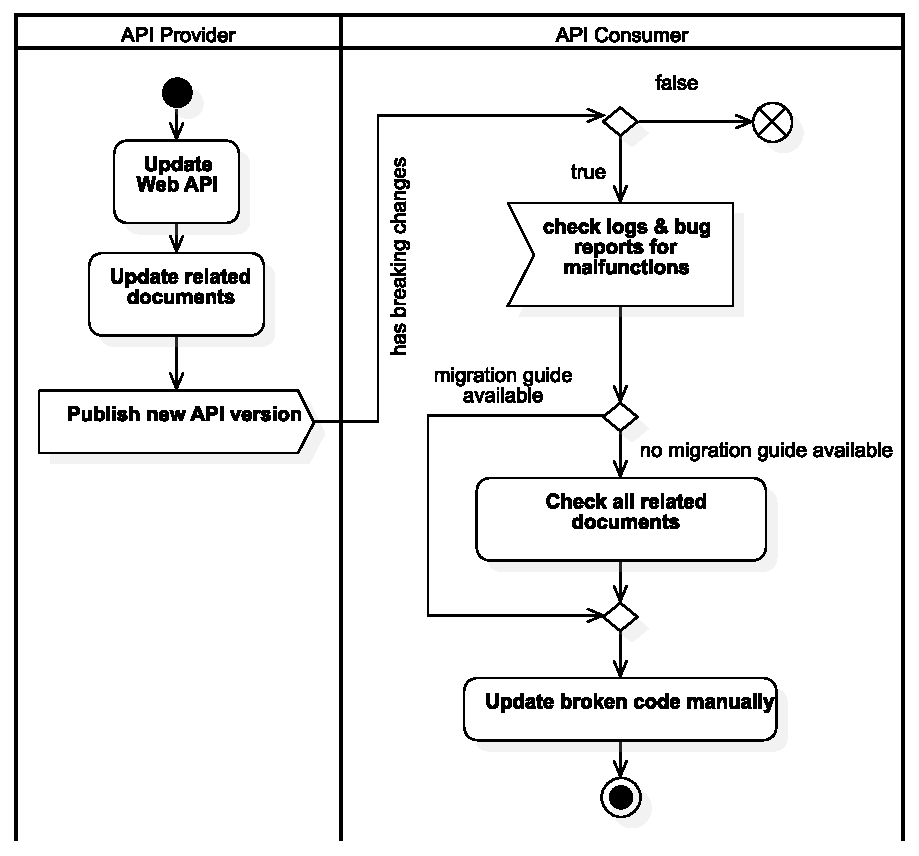
\includegraphics[width=125mm]{images/old_workflow.pdf}
		\caption{Cumbersome workflow after web service changes}
		\label{fig:oldWorkflow}
	}
\end{figure}

In a field study, Brito et. al questioned API providers on how they plan to document their changes. They found out that 22\% usually use release notes or changelogs, while only 11\% aim to provide a migration guide. Without a detailed guide that includes all of the steps required to migrate between versions, API consumers have to go through various documents and apply the modifications themselves. Resolving breaking changes manually is error-prone and leads to rising maintenance costs. A tool-based workflow could significantly shorten the time from detection to the incorporation of changes and thus reduce maintenance costs and errors.

Recent research on API evolution focuses on classifying breaking changes and patterns for Web APIs or adapting client code after updating a local library. Currently, there is a research gap regarding tool-supported workflows for migrating client applications after a Web API introduced breaking changes. Research and tools on Web API evolution have the potential to reduce development and maintenance time, improve quality and reliability of client code and prevent manually introduced bugs during the upgrade process. Automated code migration for API consumers would eliminate the need to manually inspect changes listed in change logs, newsletters, release notes or documentations and adapting the code accordingly. 
\section{Objectives}
\label{sec:Objectives}

In this thesis, we propose a new tool-supported workflow in which client code gets automatically migrated after a web service was modified. We focus on light-weight Web API technologies which can be described by an IDL, such as REST, GraphQL and gRPC. Our main objective is to facilitate the workflow shown in Figure \ref{fig:oldWorkflow} by significantly reducing the effort for API consumers. Therefore, we introduce a state-of-the-art description language to specify a machine-readable migration guide. This guide enables API providers to describe all modifications of a Web API from a previous to its latest version. In addition, we propose a tool that parses our migration guide and generates library code that is persistent to changes to its public interface once it is run for the first time. It can be used in an existing \textit{\ac{CI/CD}} pipeline or via the command line.

\begin{figure}[h]
	\centering{
		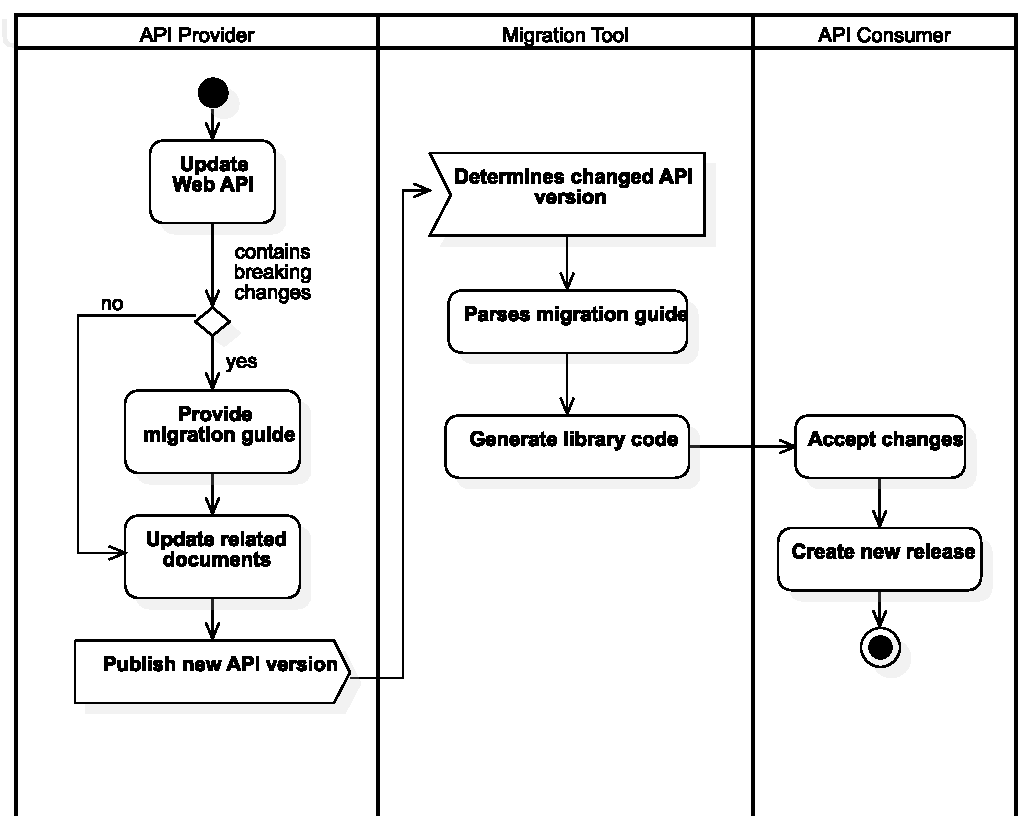
\includegraphics[width=128mm]{images/new_workflow.pdf}
		\caption{Workflow with tool support after web service changes}
		\label{fig:newWorkflow}
	}
\end{figure}

Figure \ref{fig:newWorkflow} showcases the new workflow. In addition to their current tasks, Web API providers must state all introduced changes in a machine-readable migration guide and make it available to consumers. Web API consumers have to integrate our migration tool, which automates the incorporation of changes without breaking the client application. It determines the API version from the migration guide and creates a set of rules indicating how the library should be customized to avoid introducing breaking changes to the consumer's application code. After executing these rules, the public interface of the generated library code remains unchanged and the consumer's application continues to use the library's code which acts as a facade for the lower level API calls.
\section{Outline}
\label{sec:Outline}

After the initial introduction into challenges of Web API evolution and our motivation to overcome them in Chapter \ref{ch:Introduction}, we examine the current state of related research topics in Chapter \ref{ch:RelatedWork}. Identifying the challenges in related research faciliates defining the key requirements for our proposed workflow and discovers several limitations to be aware of as Web APIs evolve. Chapter \ref{ch:RequirementsElicitation} comprises all requirements and constraints we identified from related work. In addition, we were able to derive multiple use cases from potential real-world scenarios. Taking into account all requirements and the existing related work, we create the design of our proposed system, which is described in Chapter \ref{ch:SystemDesign}. Our system is composed of multiple subsystems that each provide their own functionality. In Chapter \ref{ch:ObjectDesign} we select detailed solutions for individual subsystems by identifying either suitable third-party components or pattern templates. We instantiate our proposed system in \textsc{Pallidor}, our prototypical implementation in the Swift programming language. In Chapter \ref{ch:CaseStudyEvaluation}, we use Pallidor to migrate various types of change for a sample Web API and evaluate our proposed system based on our findings. Chapter \ref{ch:Summary} concludes the thesis and discusses future work.
\chapter{Related Work}
\label{ch:RelatedWork}

Our work relates to current research of API evolution, which focusses on classification and patterns for Web API changes. Studies were also conducted to analyze thei impact on client applications for both local libraries and Web APIs. Furthermore, research has been devoted to automating migration of breaking changes in client code for evolving local libraries. Based on insights from previous work and considering the challenges associated with Web API evolution, our research concentrates on reducing the impact of breaking changes in Web APIs on consuming applications by automating the migration process for client developers.

\section{API Evolution Patterns}
\label{sec:APIEvolutionPatterns}

Recently, in order to better understand Web API evolution, research has been devoted to classify similar kinds of changes into patterns and creating guidelines for an efficient development of Web APIs. These studies provide useful hints for determining implementation details of the migration guide specification and creating rules for automating migratory steps.

Li et al. \cite{li_how_2013} examined large popular Web APIs and defined common characteristics of changes. Their study identifies 16 change patterns, 12 of them causing compile-time errors if a high-level library is used to wrap messages on HTTP level and 4 changes causing runtime errors. They found that on average more than 50\% of the API was changed with 80\% of that breaking changes being refactorings. In addition, they identified six new challenges that arise from Web API evolution compared to local libraries. As their results show, Web APIs are less likely to change at the HTTP level than it is on their corresponding library wrappers. Hence, they suggest providing a tool that automates migration tasks at the HTTP level. These results encourage to automate the migration process, since a large part of the changes are refactorings and well-defined patterns for changes help determine the requirements for the migration guide and rules.

Exploring the challenges Web API providers are facing, Lübke et al. \cite{lubke_interface_2019} extracted eight patterns that can be applied when creating or adapting an evolution strategy for an API. These are derived from best practices found in literature and major public Web APIs \cite{lubke_interface_2019}. The authors describe different alternatives for introducing incompatible changes and advocate for using API versioning and description techniques. While one pattern does not support incompatible changes, the others balance forces of stability, potential to innovate, and maintainability for API providers. Although client developers benefit from a well-structured evolution strategy, it does not reduce the effort required to migrate between versions, especially if the API is changed frequently. By providing a machine-readable migration guide, providers would simplify their customers' workflow while maintaining the innovation potential and maintainability of their API.
\section{API Evolution Client Impact}
\label{sec:APIEvolutionClientImpact}

Client developers must devote a large extent of their efforts to keep their application compatible with an API in use. Research related to API evolution therefore also includes investigations of the impact on API consumers. Although there are studies related to the impact of changes in Web APIs, most of the studies examine applications using local libraries.

In \cite{brito_you_2020}, Brito et al. conducted a field study to determine the motivation of API providers to introduce breaking changes. They discovered that 39\% of these changes have a direct impact on consumers. The authors determined that although API providers state that the migration effort for their consumers is low (86\%) or moderate (14\%), 45\% of API-related questions were asked by client developers who have difficulties overcoming breaking changes. To find out about them, client developers need to examine a variety of documentation options as API developers plan to note their changes in release notes, change logs, source code, website, a migration guide, samples, or in a README file \cite{brito_you_2020}. In response to these challenges, API providers should focus on documenting changes in a single artifact to ease the effort of migrating for their consumers. Using a machine-readable migration manual ensures that all changes are documented in one artifact and can be easily found by consumers and tools.

Another large-scale study was conducted by Xavier et. al \cite{xavier_historical_2017}, analyzing the impact of API breaking changes in local libraries. They have seen the frequency of changes increase over time, which they associate with library development as they become more complex. Their findings show that 27.99\% of all API changes break backward compatibility. Although a median of only 2.54\% of clients are potentially affected by these changes, they have identified several outliers which show that in some cases every client application is affected. Based on their findings, they suggest using an impact analysis tool for library developers before changing commonly used APIs. While their study focuses on local libraries, the results apply to modern Web APIs as well. Furthermore, breaking backwards compatibility is a more serious problem for client developers because they cannot stick to an older version after a Web API has been updated.

Espinha et al. \cite{espinha_web_2014} further investigated the challenges for client developers regarding Web API changes. They found that the impact of changes largely depends on the quality of client application architectures. Hence, the authors prioritize separation of concerns in order to encapsulate components that are subject to change due to API development. According to their findings, the churn percentage for updating these well-designed client applications is 50\% lower than their average observations. This results in reduced efforts for maintaining an API usage, which requires at least 50\% of the initial setup effort or even exceeds it \cite{espinha_web_2014}. Hence, an automated migration process must consider the principle of separation of concerns in order to minimize the effort of integrating non-breaking changes and migrating breaking changes.
\section{API Evolution Automation}
\label{sec:APIEvolutionAutomation}

Due to the fact that adapting a client application to the latest version of an API is cumbersome, various approaches to automate the migration process have been proposed. However, automation techniques for library evolution have been rarely adopted in practice \cite[p. 300]{li_how_2013}. Li et. al divides the techniques into two categories. Operation-based tools record changes made by API providers and provide a replay function to refactor client code accordingly. The second technique analyzes changes by comparing source code and related documents of two different releases \cite[p. 306]{li_how_2013}. 

One example for an operation-based tool is \textit{CatchUp!} \cite{henkel_catchup!_2005} which creates a log of refactorings as API providers modify their code. Henkel et al. defined a trace file so that it can also be used for documentation puposes as it is in human-readable XML format and offers the option of creating an HTML document using style sheets. Their tool enables developers to replay this log to upgrade the client application by playing back the log of refactorings using its Eclipse plugin. Documenting changes in a human- and machine-readable format makes debugging easier and allows provider and consumer tools to be developed independently.

Dig et. al \cite{hutchison_automated_2006} developed the Eclipse plugin \textit{RefactoringCrawler} that automatically
detects refactorings by analyzing the source code between two versions. To increase the accuracy, their algorithm analyzes the semantics of refactor candidates. For example it detects renaming and changing of method signatures by analyzing the semantics of its call hierarchy \cite{hutchison_automated_2006}. They are able to determine seven types of refactorings with an accuracy of 85\%, focusing on rename and move modifications. 

Current academic literature on tools to automate migration refactorings is devoted to local libraries. While there are industry tools that support generating libraries in multiple languages from service specifications (e.g. OpenAPI Generator\footnote{https://openapi-generator.tech/}) and vice versa, they do not support migrating between different versions of an API. Furthermore, current automation tools do not cover new challenges introduced by Web APIs \cite[p. 306]{li_how_2013}.
\chapter{Requirements Elicitation}
\label{ch:RequirementsElicitation}

As described in Chapter \ref{ch:RelatedWork}, recent research has identified several drawbacks to modern Web APIs. Studies have been conducted, showing that their evolution has a large impact on their consumers (\cite{brito_you_2020}, \cite{xavier_historical_2017}, \cite{espinha_web_2014}). As a consequence, client developers face an increased effort to keep their application code compatible, since current tools for the automatic migration of client code (\cite{henkel_catchup!_2005}, \cite{hutchison_automated_2006}) are not applicable in a Web API context \cite{li_how_2013}. In order to better understand Web API evolution, recent studies have introduced classifications of several recurring change patterns and evolution strategies that indicate the challenges providers and consumers are facing (\cite{li_how_2013}, \cite{lubke_interface_2019}). 

Addressing these challenges, we propose introducing a tool-supported workflow as shown in Figure \ref{fig:newWorkflow} to significantly reduce the impact of Web API evolution on consumers. Therefore, a majority of migratory tasks needs to be automated according to a machine-readable migration guide which needs to be prepared in advance by providers. All changes are encapsulated in a separate library to be abstracted from client code. This library is added to client applications as a dependency. In addition, our system facilitates the workflow of API providers to release new versions by ensuring that changes to the interface do not affect consumer applications, hence providing perceived stability. The system's main objective is to combine the convenience of local libraries with the flexiblity of modern Web APIs. It aims to be seamlessly integrated into commonly used tools and workflows like continuous integration, version control and dependency management. 

Given the current and proposed workflow, multiple functional and nonfunctional requirements can directly be derived. Web API consumers use the system to automatically migrate their application between two versions. Therefore, the system needs to import a machine-readable migration guide that is delivered by Web API providers. Our analysis identified all necessary system requirements which are listed in the following section in detail. Furthermore, use cases are identified for all actors and exemplary scenarios for possible future migration scenarios are presented. All requirements and constraints are listed in section \ref{sec:Requirements} while use cases and scenarios are shown in section \ref{sec:UseCases} and section \ref{sec:Scenarios}, respectively.
\newpage
\section{Requirements}
\label{sec:Requirements}

The system consists of two key components: a migration tool and a migration guide specification. This section provides an overview of the requirements and constraints for both of them. The system must meet all of them in order to be accepted. The requirements are split into functional and nonfunctional requirements. Bruegge et. al define functional requirements "[as] the interactions between the system and its environment independent of its implementation" \cite{bruegge_object-oriented_2010}. The authors thereby describe users and external systems as part of a system's environment. Furthermore, Bruegge et al. define nonfunctional requirements "as aspects of the system that are not directly related to the functional behavior of the system" \cite{bruegge_object-oriented_2010}. They further divide nonfunctional requirements into quality requirements and constraints. 

\subsection{Functional Requirements}
\label{subsec:FunctionalRequirements}
 
 In order to enable the implementation of the workflow shown in Figure \ref{fig:newWorkflow}, both, the functional requirements of the Web API consumers and providers must be taken into account. 

\begin{itemize}[itemindent=-4pt, leftmargin=34pt, align=left]
    \item [FR1\hphantom{1}] \customlabel{fr:MigGuide}{Developing a specification for a machine-readable migration guide (FR1)} \textbf{Development of a specification for a machine-readable migration guide:} The machine-readable migration guide needs to contain all necessary information regarding changes made to the Web API. Additionally, it must provide fields to specify important meta-data like versioning information. The format of the migration guide must allow the specification of simple and complex data structures. They are required to model hierarchies within the guide or hierarchical types provided by a Web API. Changes stated within the migration guide must be distinguishable from one another by their structure. Depending on its type, a change must include fields that contain information on how to adapt the client code to maintain compatibility with the Web API.
    \item [FR2\hphantom{1}] \customlabel{fr:Configuration}{Configuration} \textbf{Provide configuration option:} A user can configure the system by providing command-line parameters or a configuration file. If applicable, a default value is used in case of a missing configuration. For each API and project, an individual configuration can be applied.
    \item [FR3\hphantom{1}] \customlabel{fr:GenLib}{Generate a client library from service specification} \textbf{Generating a client library from service specification:} A user provides a Web API specification URI as input to generate a client library which can be used by the client application. The input can either be issued locally as a file or can be remotely retrieved from the web service.
    \item [FR4\hphantom{1}] \customlabel{fr:Facade}{Providing a facade to maintain API consistency (FR4)} \textbf{Provide a facade to maintain API consistency:} A user accesses the library's functionality via a generated facade to ensure a consistent view of the API. It mimics the original interface as it uses the same method signatures and exposes them to the client application.
     \item [FR5\hphantom{1}] \customlabel{fr:AdaptFacade}{Self-adapting facade for API evolution (FR5)}
     \textbf{Self-adapting facade for API evolution:} The system automatically resolves the current version of the web service and its corresponding migration guide. If the retrieved API version differs from the local API version, the system adapts the facade according to the migration guide. As a result, users automatically receive API-related changes in their application code.
     \item [FR6\hphantom{1}] \customlabel{fr:CIInteg}{Integrate system in CI/CD}
     \textbf{Integrate system in CI/CD:} The tool will be integrated into the CI pipeline of the client application to ensure the highest level of automation. Alternatively it can be used locally via its \textit{\ac{CLI}}.
     \item [FR7\hphantom{1}] \customlabel{fr:GitInteg}{Integrate output via Git}
     \textbf{Integrate output via Git:} The modified library will be published via git pull request into the client application's repository. By publishing it, the library's version number will be incremented according to semantic versioning principles.
     \item [FR8\hphantom{1}] \customlabel{fr:MigStrategy}{Specify migration strategy}
     \textbf{Specify migration strategy:} A user can specify the migration strategy for non-migratable changes such as deletion of functionality without replacement. The selected strategy can be either provided via command-line parameters or using the configuration file. 
          \item [FR9\hphantom{1}] \customlabel{fr:OutputLang}{Specify output language}
     \textbf{Specify output language:} A user can specify the programming language in which the target library is generated. The selected output language can be either provided via command-line parameters or using the configuration file. 
\end{itemize}

\subsection{Artifacts}
\label{subsec:Artifacts}

To illustrate the artifacts from FR1 and FR4, Figure \ref{fig:migGuide} shows our proposed structure for a machine-readable migration guide and Figure \ref{fig:outcome} demonstrates the architectural composition of the code generated by our system.

\begin{figure}[h]
	\centering{
		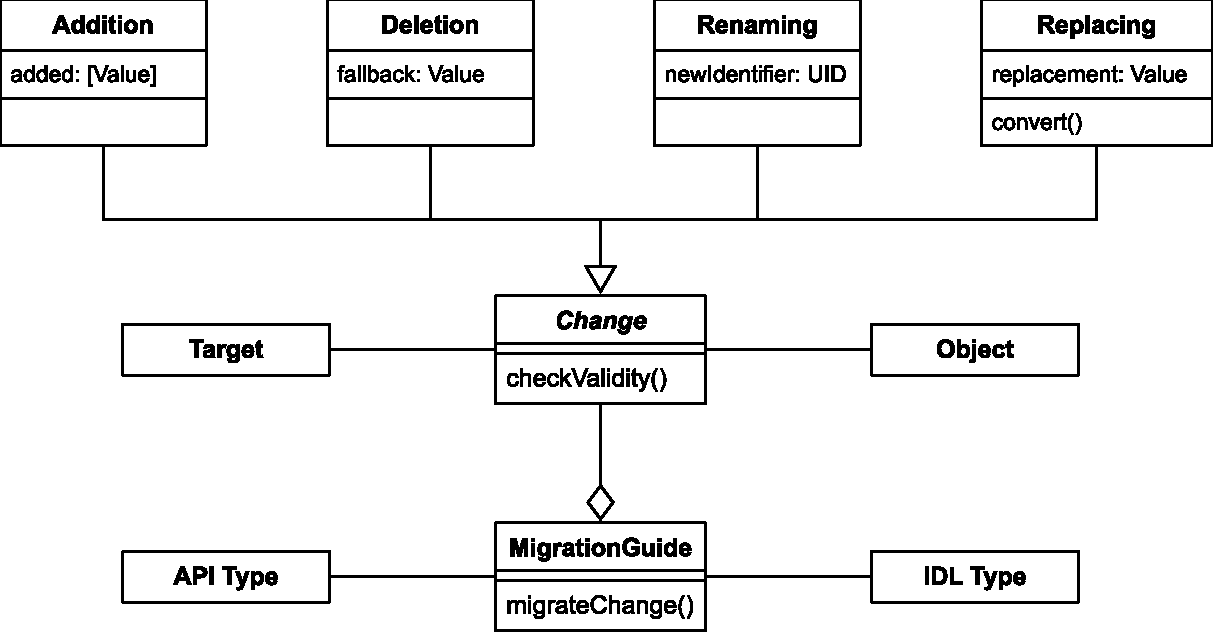
\includegraphics[width=135mm]{images/cd_migration_guide.pdf}
		\caption{Proposed structure of a machine-readable migration guide}
		\label{fig:migGuide}
	}
\end{figure}

A migration guide is responsible for migrating different types of changes that might occur due to Web API evolution. Each change must contain an identification of the object which is changed and the specific target of the change. For example, if a method parameter was changed, the method is the change object and the parameter is the change target.

\begin{figure}[!h]
	\centering{
		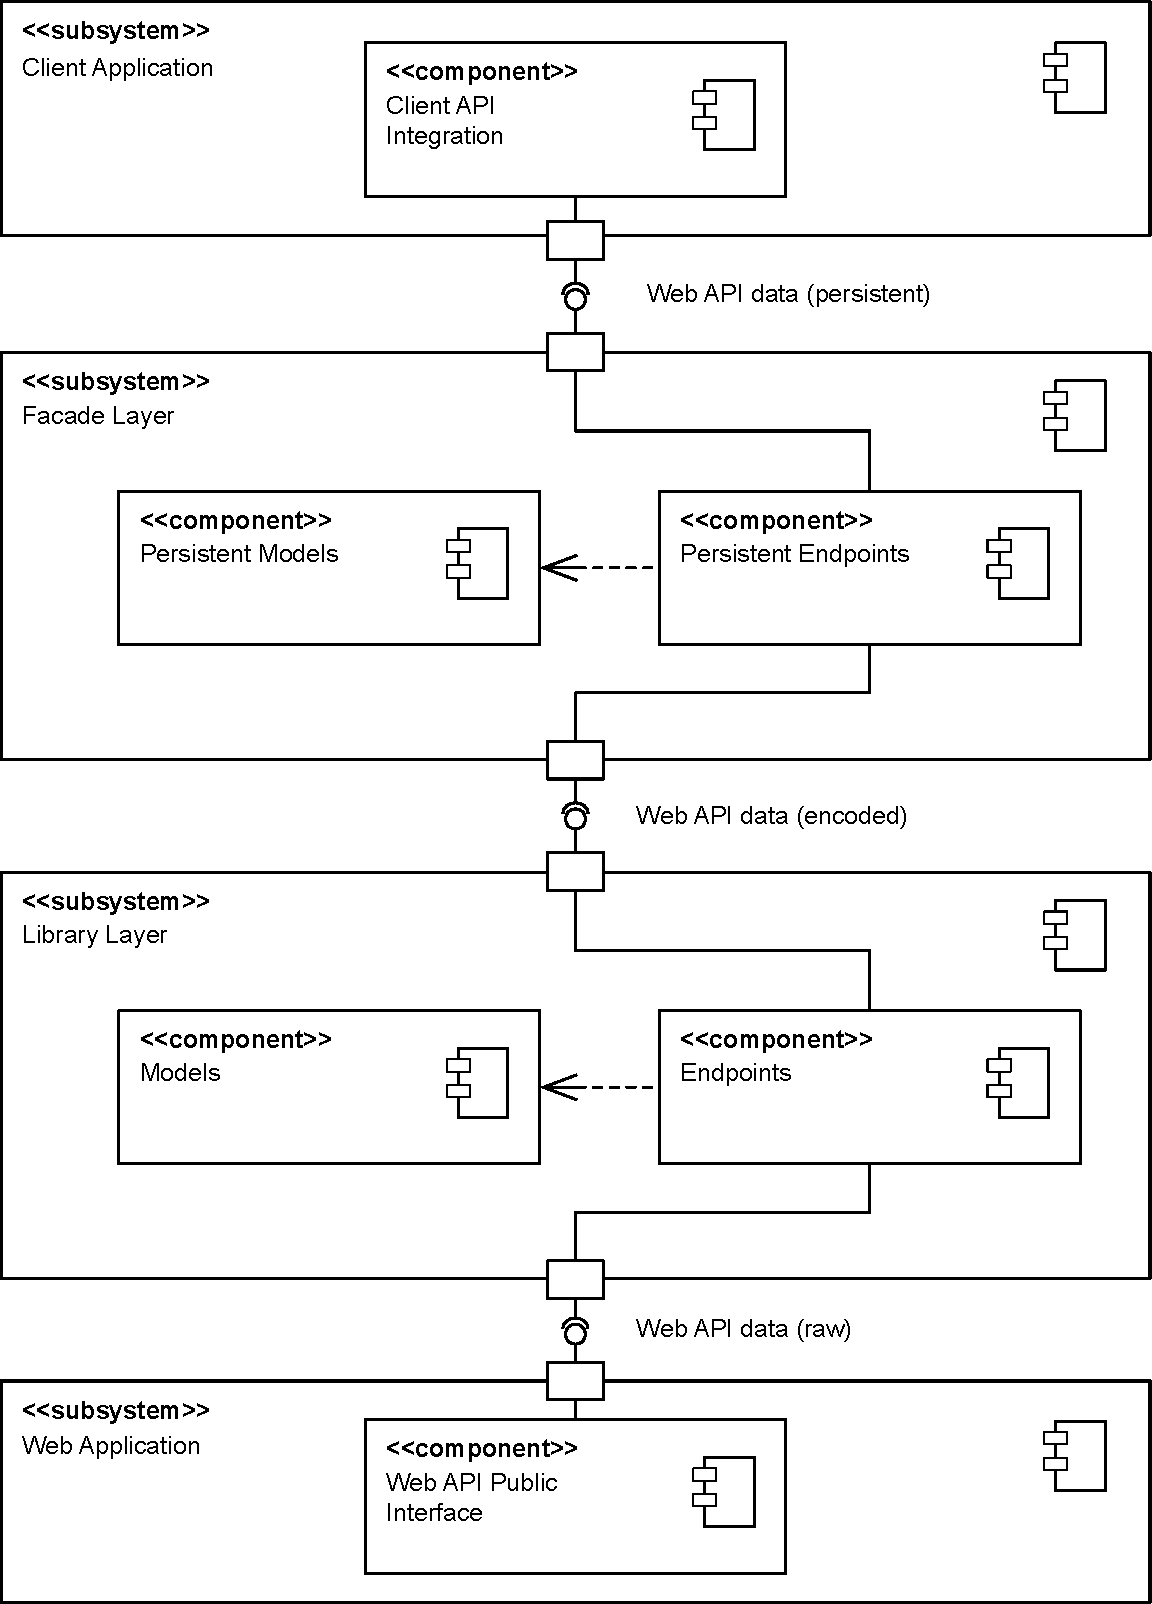
\includegraphics[width=130mm]{images/output_subsystem.pdf}
		\caption{Proposed architecture of change-proof Web API integration}
		\label{fig:outcome}
	}
\end{figure}

The output of our system is designed in a layered architectural style in order to incorporate changes made to the Web API without affecting the client application. Due to the fact that Web APIs are already integrated using a layered network architecture, introducing additional layers does not affect current development practices. The library subsystem is a local representation of the Web API and provides its services only to the facade subsystem. The facade subsystem uses them to issue HTTP requests to the Web API while maintaining a stable interface to the client application. When changes are introduced to the Web API, the library subsystem gets updated accordingly and the API contract between the library and facade subsystems is broken. For fixing the API contract, all changes stated in the migration guide modify the internal functionality of the facade subsystem without altering any publicly exposed interfaces. 

\subsection{Nonfunctional Requirements}
\label{subsec:NonfunctionalRequirements}
The following requirements were defined to ensure a high quality system. As described in \cite{bruegge_object-oriented_2010}, each requirement relates to one or more of the categories usability, reliability or supportability. According to the authors, supportability includes adaptability and maintainability.

\begin{itemize}[itemindent=-13pt, leftmargin=43pt, align=left]
    \item [NFR1\hphantom{1}] \customlabel{nfr:CodeStyle}{NFR1 (Code Style)} \textbf{Code Style:} All code generated by the system must follow a linting ruleset predefined in a configuration file to increase maintainability.
    \item [NFR2\hphantom{1}] \customlabel{nfr:ClientDocumentation}{NFR2} \textbf{Documentation of facade:} To increase usability for client application developers, the facade's public interface will be documented using code comments. These comments explain the usage of the Web API and are derived from its IDL document.
    \item [NFR3\hphantom{1}] \customlabel{nfr:SystemDocumentation}{NFR3} \textbf{Documentation of system:} To increase maintainability, the system will be documented using code comments. Documentation will be auto-gen\-erated and summarized in the \texttt{README.md} file.
    \item [NFR4\hphantom{1}] \customlabel{nfr:TestCoverage}{Test Coverage (NFR4)} \textbf{Test coverage:} To ensure the system's robustness, unit tests must be provided for all supported migration types. Additionally, unit test must be provided with respect to different migration strategies. Special attention needs to be paid to edge cases.
    \item [NFR5\hphantom{1}] \customlabel{nfr:Coloring}{NFR5}
    \textbf{Coloring of key messages:} Key output messages of the system will be highlighted using coloring schemes to increase usability.
    \item [NFR6\hphantom{1}] \customlabel{nfr:Help}{NFR6}
    \textbf{Help messages:} The system provides detailed instructions on how to use its command-line interface. The help will be available via \texttt{help} command. This ensures that users are able to easily learn how to operate the system.
    \item [NFR7\hphantom{1}] \customlabel{nfr:CodeVersion}{NFR7}
    \textbf{Code version:} The system is constrained to issuing language-specific library code in the language's current major version. This improves adaptability when client applications are using the latest version of a programming language.
    \item [NFR8\hphantom{1}] \customlabel{nfr:Dependencies}{NFR8}
    \textbf{Dependency Management:} Language-specific implementations are required to use a dependency manager to manage all third party libraries. Using a dependency manager increases maintainability significantly because dependency meta information provides a single source of truth.
        \item [NFR9\hphantom{1}] \customlabel{nfr:MigGuideFormat}{NFR9 (Migration Guide Format)}
    \textbf{Migration guide format:} The migration guide needs to be specified in a human-readable format which web developers are familiar with. Using a domain-specific language increases acceptance and usability especially for debugging and manual inspection. Additionally, utilizing a format that is already widely used in the software development industry has the advantage that IDEs provide convenient features such as syntax highlighting or auto-completion.
        \item [NFR10\hphantom{1}] \customlabel{nfr:UserInput}{NFR10}
    \textbf{Handling user input:} Missing or incorrect configuration parameters trigger a detailed error message so that the user can easily examine and correct the configuration.
\end{itemize}

\subsection{Constraints}
\label{subsec:Constraints}

For the system to work properly, some constraints have to be fulfilled. A constraint is a nonfunctional requirement that has been specified in advance by external factors and must be reconciled with other affected design decisions \cite{bass_software_2013}.

\begin{itemize}[itemindent=-13pt, leftmargin=43pt, align=left]
    \item [C1\hphantom{1}] \customlabel{nfr:Legal}{C1} \textbf{Legal requirements}: All dependencies must be available under MIT license regulations so that the system can also be published under the MIT license.
    \item [C2\hphantom{1}] \customlabel{nfr:Operations}{NFR2} \textbf{Operations requirements}: An IDL document describing the public interface of an API must be available in order to generate library code. Furthermore, both the API consumers and producers need to follow semantic versioning\footnote{see https://semver.org/} principles.
    \item [C3\hphantom{1}] \customlabel{nfr:Implementation}{NFR3} \textbf{Implementation requirements}: API consumers have to use GitHub as their version control system to use the system as a GitHub action in their CI/CD pipeline. Additionally, it is provided as a command-line program without a graphical user interface. This enables local execution or integration into other CI/CD tools.
\end{itemize}

\section{Use Cases}
\label{sec:UseCases}

After identifying requirements and constraints to enable an improved workflow for Web API consumers and providers, we derived use cases from their common interactions with our proposed system. Bruegge et. al define Use Cases as "general sequences of events that describe all the possible actions between an actor and the system for a given piece of functionality" \cite{bruegge_object-oriented_2010}.

For a better illustration we provide a use case diagram for both actors. Figure \ref{fig:useCaseConsumer} shows the typical use cases of our system from a Web API consumer's perspective.

\begin{figure}[h]
	\centering{
		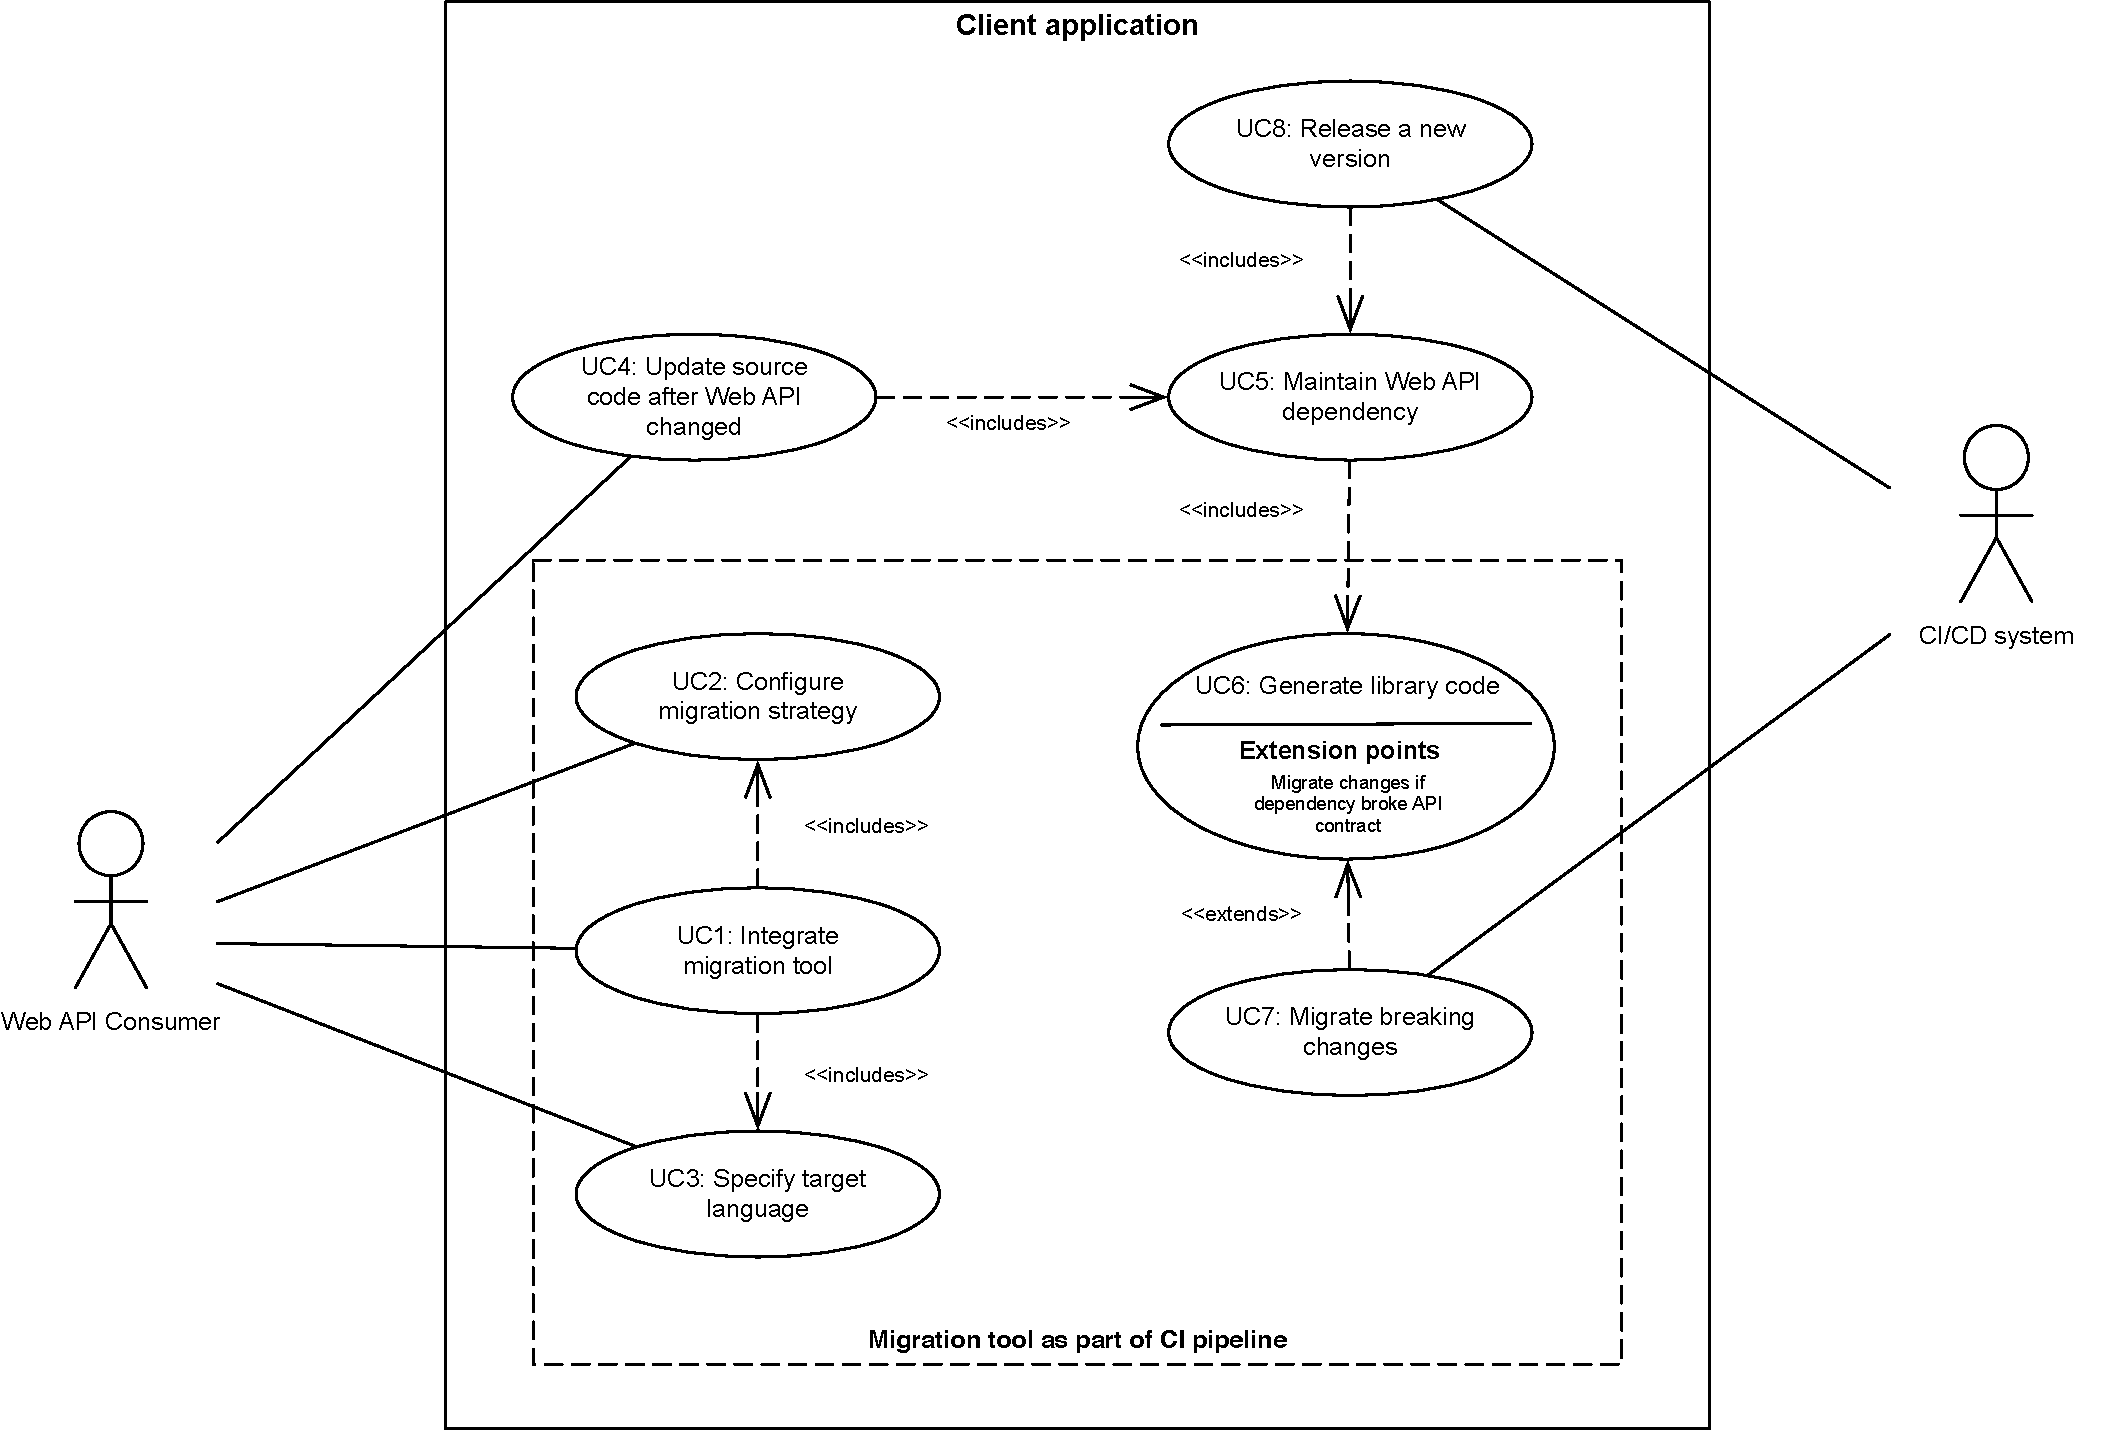
\includegraphics[width=155mm]{images/usecase_consumer.pdf}
		\caption{Use cases of Web API consumers}
		\label{fig:useCaseConsumer}
	}
\end{figure}

The migration tool is modeled as a subsystem of the client application due to its integration into the application's CI/CD pipeline. Integrating the tool requires Web API consumers to specify the target programming language for the generated library code. Furthermore, a migration strategy can be configured to meet the specific needs of the client project. Although both activities are part of the integration use case, they are modeled explicitly for client projects that do not use a CI/CD pipeline. 

Updating source code after a Web API dependency changed is the most important use case for Web API consumers. In addition to generating library code from a Web API's IDL document, our system migrates all changes as stated in its migration guide. This migration guide is created and published by Web API providers. The corresponding use case (\texttt{UC11}) is shown in figure \ref{fig:useCaseProvider}. 

The CI/CD system is modeled as a separate actor to illustrate the use cases that do not require manual interaction by client developers. Its primary task is to create a release of a new version of the client application without breaking changes that were introduced in the Web API. Therefore, it automatically migrates all of these changes by using our system.

For further explanation, the two most important use cases for Web API consumers are described in detail below.
\newpage
\subsubsection{Integrate Migration Tool}
\label{subsubsec:UseCase:IntegrateTool}

\vspace{-2mm}
\begin{center}
    \def\arraystretch{1.5}
    \begin{longtable}{ p{0.22\linewidth} p{0.72\linewidth} }
    \hline
        \textit{Source} & Web API consumer\\
    \hline
        \textit{Stimulus} & Client application needs to incorporate and persist a Web API. \\
    \hline
    	\textit{Environment} & \textbf{Preconditions:} The client application uses a CI / CD pipeline into which the migration tool can be integrated. The interface of the desired Web API is described using an IDL document.
    	
    	\textbf{Postcondition:} The resulting library must be added as a dependency to the client application.
    	\\
    \hline
    	\textit{Artefact} & Migration tool\\
    \hline
    \textit{Response} &
    \vspace{-5.1mm}
    \begin{enumerate}[itemindent=-9pt, leftmargin=14pt, itemsep=0pt, align=left]
    	\item The migration tool gets integrated as part of the CI/CD pipeline of the client application. Therefore, its configuration is either provided as a file via URI or via \ac{CLI} parameters. Optionally, a code formatting ruleset can be specified via its configuration file URI.
        \item The migration tool retrieves the IDL document from its URI.
        \item The migration tool parses the information from the IDL document and generates library code encapsulating lower level HTTP calls. This code is for internal use only and cannot be accessed publicly.
        \item The migration tool generates a public facade layer to persist the current view on the Web API by abstracting calls to the previously generated library code. 
        \item The migration tool generates related meta files to facilitate integrating the output via dependency management.
    \end{enumerate} \\ [-5mm]
    \hline
    \textit{Response Measure} &
    \vspace{-8.5mm}
    \begin{itemize}[itemindent=-9pt, leftmargin=14pt, itemsep=0pt, align=left]
       	\item Error: Execution fails if the IDL document is unavailable or incorrect.
       	\item Success: Output compiles and requests/responses to/from the Web API are processed without errors. 
        \vspace{-5mm}
    \end{itemize}\\
    \hline
    \end{longtable}
\end{center}
\newpage
\subsubsection{Update Source Code After Service Change}
\label{subsubsec:UseCase:FixClientApp}

\vspace{-2mm}
\begin{center}
    \def\arraystretch{1.5}
    \begin{longtable}{ p{0.22\linewidth} p{0.72\linewidth} }
    \hline
        \textit{Source} & Web API consumer\\
    \hline
        \textit{Stimulus} & The client application crashes after a modified Web API is published.\\
    \hline
    	\textit{Environment} & \textbf{Preconditions:} 
    	\begin{itemize}
    		\item The client application integrates a Web API via library code generated by our migration tool. 
    		\item Execution is either triggered manually or as part of a CI/CD pipeline of the client application. 
    		\item The latest release of a Web API introduced breaking changes either to its public interface or behavior. 
    		\item The Web API provider published a machine-readable migration guide along with an updated IDL document.
    	\end{itemize}
    	
    	\textbf{Postcondition:} Client application's dependency must be updated to use the latest version of the generated library code.
    	\\
    \hline
    	\textit{Artefact} & Migration tool\\
    \hline
    \textit{Response} &
    \vspace{-5.1mm}
    \begin{enumerate}[itemindent=-9pt, leftmargin=14pt, itemsep=0pt, align=left]
        \item The migration tool retrieves the updated IDL document and the migration guide from their URIs.
        \item The migration tool checks the changes specified in the migration guide for consistency and correctness. If this check fails, execution is aborted and an error is raised.
        \item The migration tool parses the information from the IDL document and generates library code encapsulating lower level HTTP calls. This code is for internal use only and cannot be accessed publicly.
        \item The migration tool uses the information from the migration guide to adapt the behavior of the previously generated facade layer without modifying the public interface of the facade.
        \item The migration tool generates related meta files to facilitate integrating the output via dependency management.
    \end{enumerate} \\ [-5mm]
    \hline
    \textit{Response Measure} &
    \vspace{-8.5mm}
    \begin{itemize}[itemindent=-9pt, leftmargin=14pt, itemsep=0pt, align=left]
    	\item Error: Execution fails if the IDL document is unavailable or incorrect.
       	\item Error: Execution fails if changes stated in the migration guide are contradicting or incompatible.
       	\item Success: Output compiles and requests/responses to/from the Web API are processed without errors. 
        \vspace{-5mm}
    \end{itemize}\\
    \hline
    \end{longtable}
\end{center}

Web API providers are the second group of actors that participate in our proposed workflow. Figure \ref{fig:useCaseProvider} shows the typical use cases of our system from their perspective.

\begin{figure}[h]
	\centering{
		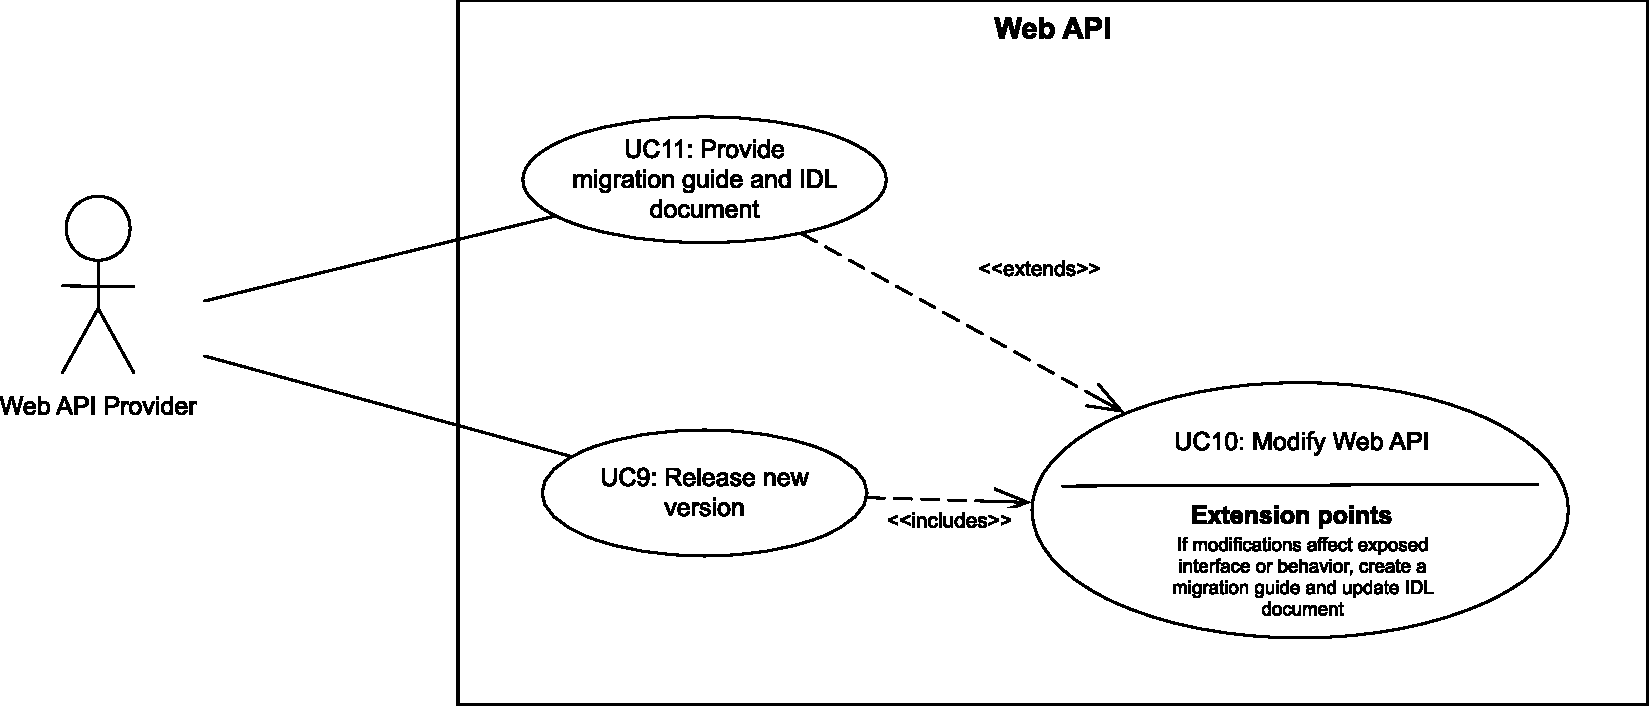
\includegraphics[width=150mm]{images/usecase_provider.pdf}
		\caption{Use cases of Web API providers}
		\label{fig:useCaseProvider}
	}
\end{figure}

Web API providers need to decide whether to introduce breaking changes to the publicly available interface or behavior. When breaking changes cannot be avoided, providers must create a machine-readable migration guide that specifies them. Furthermore, they need to provide an updated IDL document describing the current state of the Web API. Since our proposed workflow is only slightly different from their current workflow, a detailed description of a provider's use case focuses on providing a migration guide and an IDL document.

\subsubsection{Provide Migration Guide and IDL document}
\label{subsubsec:UseCase:MigGuideIDL}

\vspace{-2mm}
\begin{center}
    \def\arraystretch{1.5}
    \begin{longtable}{ p{0.22\linewidth} p{0.72\linewidth} }
    \hline
        \textit{Source} & Web API provider\\
    \hline
        \textit{Stimulus} & New functionality was added to the Web API or existing behavior was changed. Therefore, a new version of the Web API is released. \\
    \hline
    	\textit{Environment} & \textbf{Preconditions:} The provider introduced breaking changes to the exposed interface or behavior when modifying the Web API.
    	
    	\textbf{Postcondition:} The output needs to be published on a publicly accessible server and its URI has to be provided to Web API consumers.
    	\\
    \hline
    	\textit{Artefact} & Migration guide, IDL document\\
    \hline
    \textit{Response} &
    \vspace{-5.1mm}
    \begin{enumerate}[itemindent=-9pt, leftmargin=14pt, itemsep=0pt, align=left]
    	\item The IDL document must describe the publicly exposed interface and behavior. The Web API provider can either manually create this document or generate it using tools.
    	\item The migration guide must contain the type of IDL used to describe the Web API.
    	\item The migration guide must contain the type of Web API.
    	\item The migration guide must contain both the previous and the current version number according to the semantic versioning principles.
    	\item The migration guide can contain a short textual summary to provide an overview of the changes introduced in the current version.
    	\item The migration guide must contain a list of all breaking changes introduced in the current version. 
    \end{enumerate} \\ [-5mm]
    \hline
    \textit{Response Measure} &
    \vspace{-8.5mm}
    \begin{itemize}[itemindent=-9pt, leftmargin=14pt, itemsep=0pt, align=left]
       	\item Success: The migration guide can be retrieved and parsed by migration tool.
       	\item Success: The IDL document can be retrieved and parsed by migration tool.
        \vspace{-5mm}
    \end{itemize}\\
    \hline
    \end{longtable}
\end{center}

Currently, Web API providers have to manually create a migration guide. We propose that future research should explore automating this task to reduce the effort for providers. Existing tools for automatic generation of IDL documents can serve as a reference here.
\newpage
\section{Scenarios}
\label{sec:Scenarios}
According to Bruegge et. al, scenarios are instances of use cases describing a concrete set of actions \cite{bruegge_object-oriented_2010}. In the following section we present three example scenarios for possible uses of our system. They are intended to demonstrate how Web API providers and consumers can use our tool to simplify their respective workflows and meet the challenges of the independent evolution processes.

\subsubsection{Migrating an iOS application}
\label{subsubsec:Scenario:RESTScenario}

\textit{Simplified migration process in an iOS application that uses a REST API backend for storing and retrieving notes.}
\medskip
\\The iOS application "MyNotesApp" published by NoteMe Ltd. uses a REST API backend to store and retrieve the notes of its users. The backend utilizes the OpenAPI specification to describe its publicly exposed interface and behavior. Both systems are developed by individual teams that incorporate our migration tool into their workflow. Both code bases are located in separate repositories on GitHub\footnote{https://www.github.com/}. After Alice, a developer from the backend team, published a new version of the REST API, she provides two URIs located on the same web server pointing to the updated OpenAPI specification and a migration guide. Since new business demands required her to modify the application's data models, breaking changes were introduced that she specified in the migration guide. Bob, a member of the frontend developer team is aware of these breaking changes, but he cannot apply all changes manually because the frontend team faces staffing shortage. However, our migration tool is part of the CI pipeline as a GitHub action, which automatically migrates all changes and generates updated library code that is submitted via git pull request to its own repository on GitHub. Since the iOS application uses the Swift Package Manager to maintain its dependencies, the updated library code is automatically incorporated after the frontend team accepted the pull request. A new release is created by the CD system and Claire, the tech leader of "MyNotesApp" publishes the app to the Apple AppStore.
\subsubsection{Migrating a web application using a third party service}
\label{subsubsec:Scenario:gRPCScenario}

\textit{Simplified migration process in a web application that uses a public gRPC-based API provided by Google to create 3D animated GIFs.}
\medskip
\\ The social media platform "Yearbook" is a web application written in TypeScript, that enables users to share the most important milestones of their year. It differs from other platforms in that the number of posts per user is limited to 12 posts per year. SocialViz Inc., the company behind Yearbook, identified that its customers want to use animated GIFs to celebrate their birthdays with their friends and families with an eye-catching post. Creating a GIF is an inconvenient process for their users. Fortunately, Google LLC provides "gifinator", a public service that allows client applications to create animated 3D GIFs by sending gRPC-based messages with parameters specifying the style of these animations. Lucas, a developer on the Yearbook frontend team, is responsible for integrating this interface. Since Google released the API in a beta version, it is subject to frequent, unannounced changes, namely renaming of public operations. Lucas spends a large share of his working hours adjusting the interface to adapt to these changes while his other tasks remain unfinished. To meet these challenges, he integrates our tool into the CI pipeline of Yearbook. Thereby, all changes are automatically incorporated and abstracted, generating a stable interface that client code can rely on. To make this possible, Google offers a machine-readable migration guide and an updated \texttt{.proto} file, that are fetched by our system. Since the generated output is built into the Yearbook as a JavaScript library, updating this dependency can easily be done by Lucas, who publishes it on a web server.
\subsubsection{Automating migration documentation for Web API providers}
\label{subsubsec:Scenario:graphQLScenario}

\textit{Simplified evolution process for the provider of a GraphQL-based Web API by generating a machine-readable migration guide that can be used by the consumer's tools}
\medskip
\\ "Unsensored" is an application of the startup Ingenuitees. It collects and analyzes sensor information from industrial machines to predict the need for maintenance activities. After they built a solid customer base and sufficient industry knowledge, they want to expand their services to new potential customers. Therefore, they decided to create a monetized Web API that allows to query analytical information using the GraphQL query language and incorporate the responses in client applications. As they work closely with their customers, Amanda, Ingenuitees 'senior developer, presents their plan to Drew, a developer responsible for integrating third-party services at OnTrack Ltd., one of Ingenuitees' key customers. Although Drew likes this idea, he points out that OnTrack Ltd. has strict requirements for the stability of API contracts. These requirements are at odds with Ingenuitee's entrepreneurial spirit and agile development processes. Therefore, Amanda wants to ensure that new features can be added frequently while deprecated features can be changed without breaking client applications. Drew advises her that he has included our proposed system in their application's CI pipeline to automatically migrate other third-party Web APIs. For this to work, Amanda would have to state every change in a machine-readable migration guide and provide it along with the new version and IDL document. They agree to develop a proof of concept, whereupon Amanda begins to gather information regarding the creation of a migration guide. She finds that by comparing the differences in the schema definitions of two versions of their API, she can develop an algorithm to generate a machine-readable migration guide. She integrates this algorithm as a Github action into the CI pipeline of the Web API and publishes the result along with the updated schema definition on a staging web server. Drew uses our system to integrate the Web API of "Unsensored" in their test environment. After verifying that the migrations are done correctly, Amanda publishes the Web API for production.
\chapter{System Design}
\label{ch:SystemDesign}

After analyzing functional and nonfunctional requirements, identifying use cases and possible usage scenarios, this chapter focusses on creating a system design model derived from the specifications of the analysis model. The resulting system design artifact forms the foundation for the subsequent object design analysis.

In order to achieve the best possible quality of our proposed system and its output, the criteria identified from Section \ref{sec:Requirements} must be evaluated and balanced with regard to their applicability. Demands that have not been considered up to now as well as contradicting requirements must be incorporated or resolved. Therefore, the design goals of our system are defined in Section \ref{sec:DesignGoals} and prioritized to maximizie the possible benefit for all stakeholders. 

Considering all functionality and quality criteria defined during requirements analysis results in a complex system that is difficult to develop and maintain as a whole. In order to distribute the workload among development teams and to facilitate training of new team members, subsystems need to be identified that support a clear separation of concerns and can be maintained independently. We identified a composition of subsystems in which each subsystem provides well-defined interfaces to its encapsulated internal functionality. Section \ref{sec:SubsystemDecomposition} contains the details of the interactions between subsystems and gives an overview of the modular architecture of our proposed system.

Our system is supposed to be executed as an additional step during the build stage in an existing CI/CD pipeline. While it is designed to run automatically, various boundary conditions require manual intervention of the user in order to resolve errors in the configuration or during runtime. Integrating the system into an existing CI/CD pipeline and troubleshooting for occuring errors is described in detail in Section \ref{sec:BoundaryConditions}.

In Section \ref{sec:HardwareSoftwareMapping} an exemplatory execution environment is used to demonstrate the flexibility of the subsystem decomposition. Therefore, its abstract components are mapped to representational subsystems that could be applied in this execution environment. In addition, all modified services and resulting artifacts are described in detail.
\newpage
\section{Design Goals}
\label{sec:DesignGoals}

The main purpose of our system is to facilitate the evolution process of Web APIs. Therefore, it must meet several requirements in order to be of real benefit to all actors involved. Some of these requirements are not complementary but contradict each other. In order to achieve the best possible result for our users, we prioritize our design decisions in the following section.

\paragraph{Dependability Criteria}
Decisions about the dependability of the system concern the effort to be invested in minimizing system crashes and their effects on users \cite{bruegge_object-oriented_2010}. Integrating our system into the CI/CD pipeline of an application means that subsequent process steps rely on its error-free execution. Emphasis is therefore on \ref{nfr:TestCoverage} which implies creating extensive tests of the migration logic, especially with regard to edge cases. In addition, incorrect user input must be handled and detailed error messages must be provided so that users can identify and correct errors themselves. By prioritizing robustness and fault tolerance, the delivery time for new functionality in our system, such as additional language or API type support, is significantly extended. 

Furthermore, client applications rely on an error-free execution of the code emitted by our system. Therefore, the resulting library code needs to handle internal errors appropriately and forward any response emitted by the Web API.  As it is designed to mirror the behavior of the Web API, also any errors that are issued by the Web API are returned to the requesting method within client code. Hence, client developers are responsible for handling errors appropriately and designing their application for failures. 

\paragraph{Performance Criteria}
Achieving high performance measures is not an essential requirement of our system as it runs as a background process in an application's CI/CD pipeline or in a user's local terminal. While users do not depend on fast response times or a high throughput, the memory usage of our system increases with the size of the IDL document or migration manual. Therefore, when designing the system architecture, care should be taken that memory-intensive components are encapsulated as this provides the possibility to replace them with more efficient algorithms if necessary. In terms of the library code generated, our design choices \ref{fr:Facade} and \ref{fr:AdaptFacade} result in decreased performance for client applications as API requests and responses must be processed across multiple layers.

\paragraph{Maintenance Criteria}
According to Bruegge et. al, maintenance design decisions determine the difficulty of changing a system after its initial deployment \cite{bruegge_object-oriented_2010}. Well-defined subsystems that enable a clear separation of concerns ensure that our system maintains a high degree of extensibility and modifiability. In particular, components concerned with the language-specific generation of libraries or the import of different types of IDLs must be designed with strict consideration of extensibility. This is due to the fact that supporting more languages and types of APIs is critical to increasing our system's adoption and adding additional value to its users. The encapsulation of language or API-specific functionality also improves the modifiability of our system by limiting changes due to external influences to the corresponding component. 

Focussing on expandability and modifiability involves a trade-off in terms of portability and adaptability. Adapting the system to another application domain, e.g. managing API evolution for providers is not intended. Furthermore, the support of different types of language-specific library generation for several Web API styles increases the complexity of the system, which means that the effort for new maintainers to understand the system is increased. Porting it to other platforms which implies using a different host language becomes more complicated. 

Although we do not consider any cost criteria in this thesis, it is important to note that our maintenance criteria together with an extensive testing result in longer delivery times with significantly higher costs for development and maintenance. Using the output of our system, on the other hand, reduces development costs and delivery times of client applications, as switching between different API types and programming languages is frictionless, an according implementation of our system implied. In order to be able to use the generated code for a different application domain, programming language or API type, our system just requires the corresponding parameters and does not need any adaptation of its functionality.

\paragraph{End User Criteria}
Reducing the manual overhead of evolution for Web API consumers is the main goal of our proposed system. Automating the workflow for migrating client applications adds an additional task for Web API providers. By requiring them to specify all changes in a migration guide for each release, the effort of consumers is shifted to the provider side. This design decision was made based on the assumption that future research can concentrate on automating the creation of a migration guide for Web API providers. Related research as shown in section \ref{sec:APIEvolutionAutomation} demonstrates how capturing and replaying or comparing techniques can be used to realize possible scenarios like scenario \ref{subsubsec:Scenario:graphQLScenario}. In addition, the number of consumers of public Web APIs is exceeding their providers, resulting in an overall reduction in maintenance effort. 

To maximize the positive impact of the system, special attention is paid to its usability for Web API consumers. Nonfunctional requirements were specified for coloring of key output messages (\ref{nfr:Coloring}), documentation of generated library code (\ref{nfr:ClientDocumentation}) and provision of help messages (\ref{nfr:Help}) to ensure a high degree of usability. All of the code emitted by our system is documented by code comments that explain how to use the Web API thus facilitating learning for users.
\newpage
\section{Subsystem Decomposition}
\label{sec:SubsystemDecomposition}

By dividing our system into smaller subsystems, the workload can be distributed among development teams and components that are already available to developers can be reused. The subsystems were identified by analyzing the flow of events shown in Figure \ref{fig:useCaseConsumer} and \ref{fig:useCaseProvider}. Each subsystem has precisely defined interfaces that are provided to its consumers and thus enable a modular architecture in which subsystems can easily be replaced by more efficient alternatives. Furthermore, our design enables implementations that support importing multiple IDL types and generating output for multiple programming languages at the same time. 

\begin{figure}[h]
	\centering{
		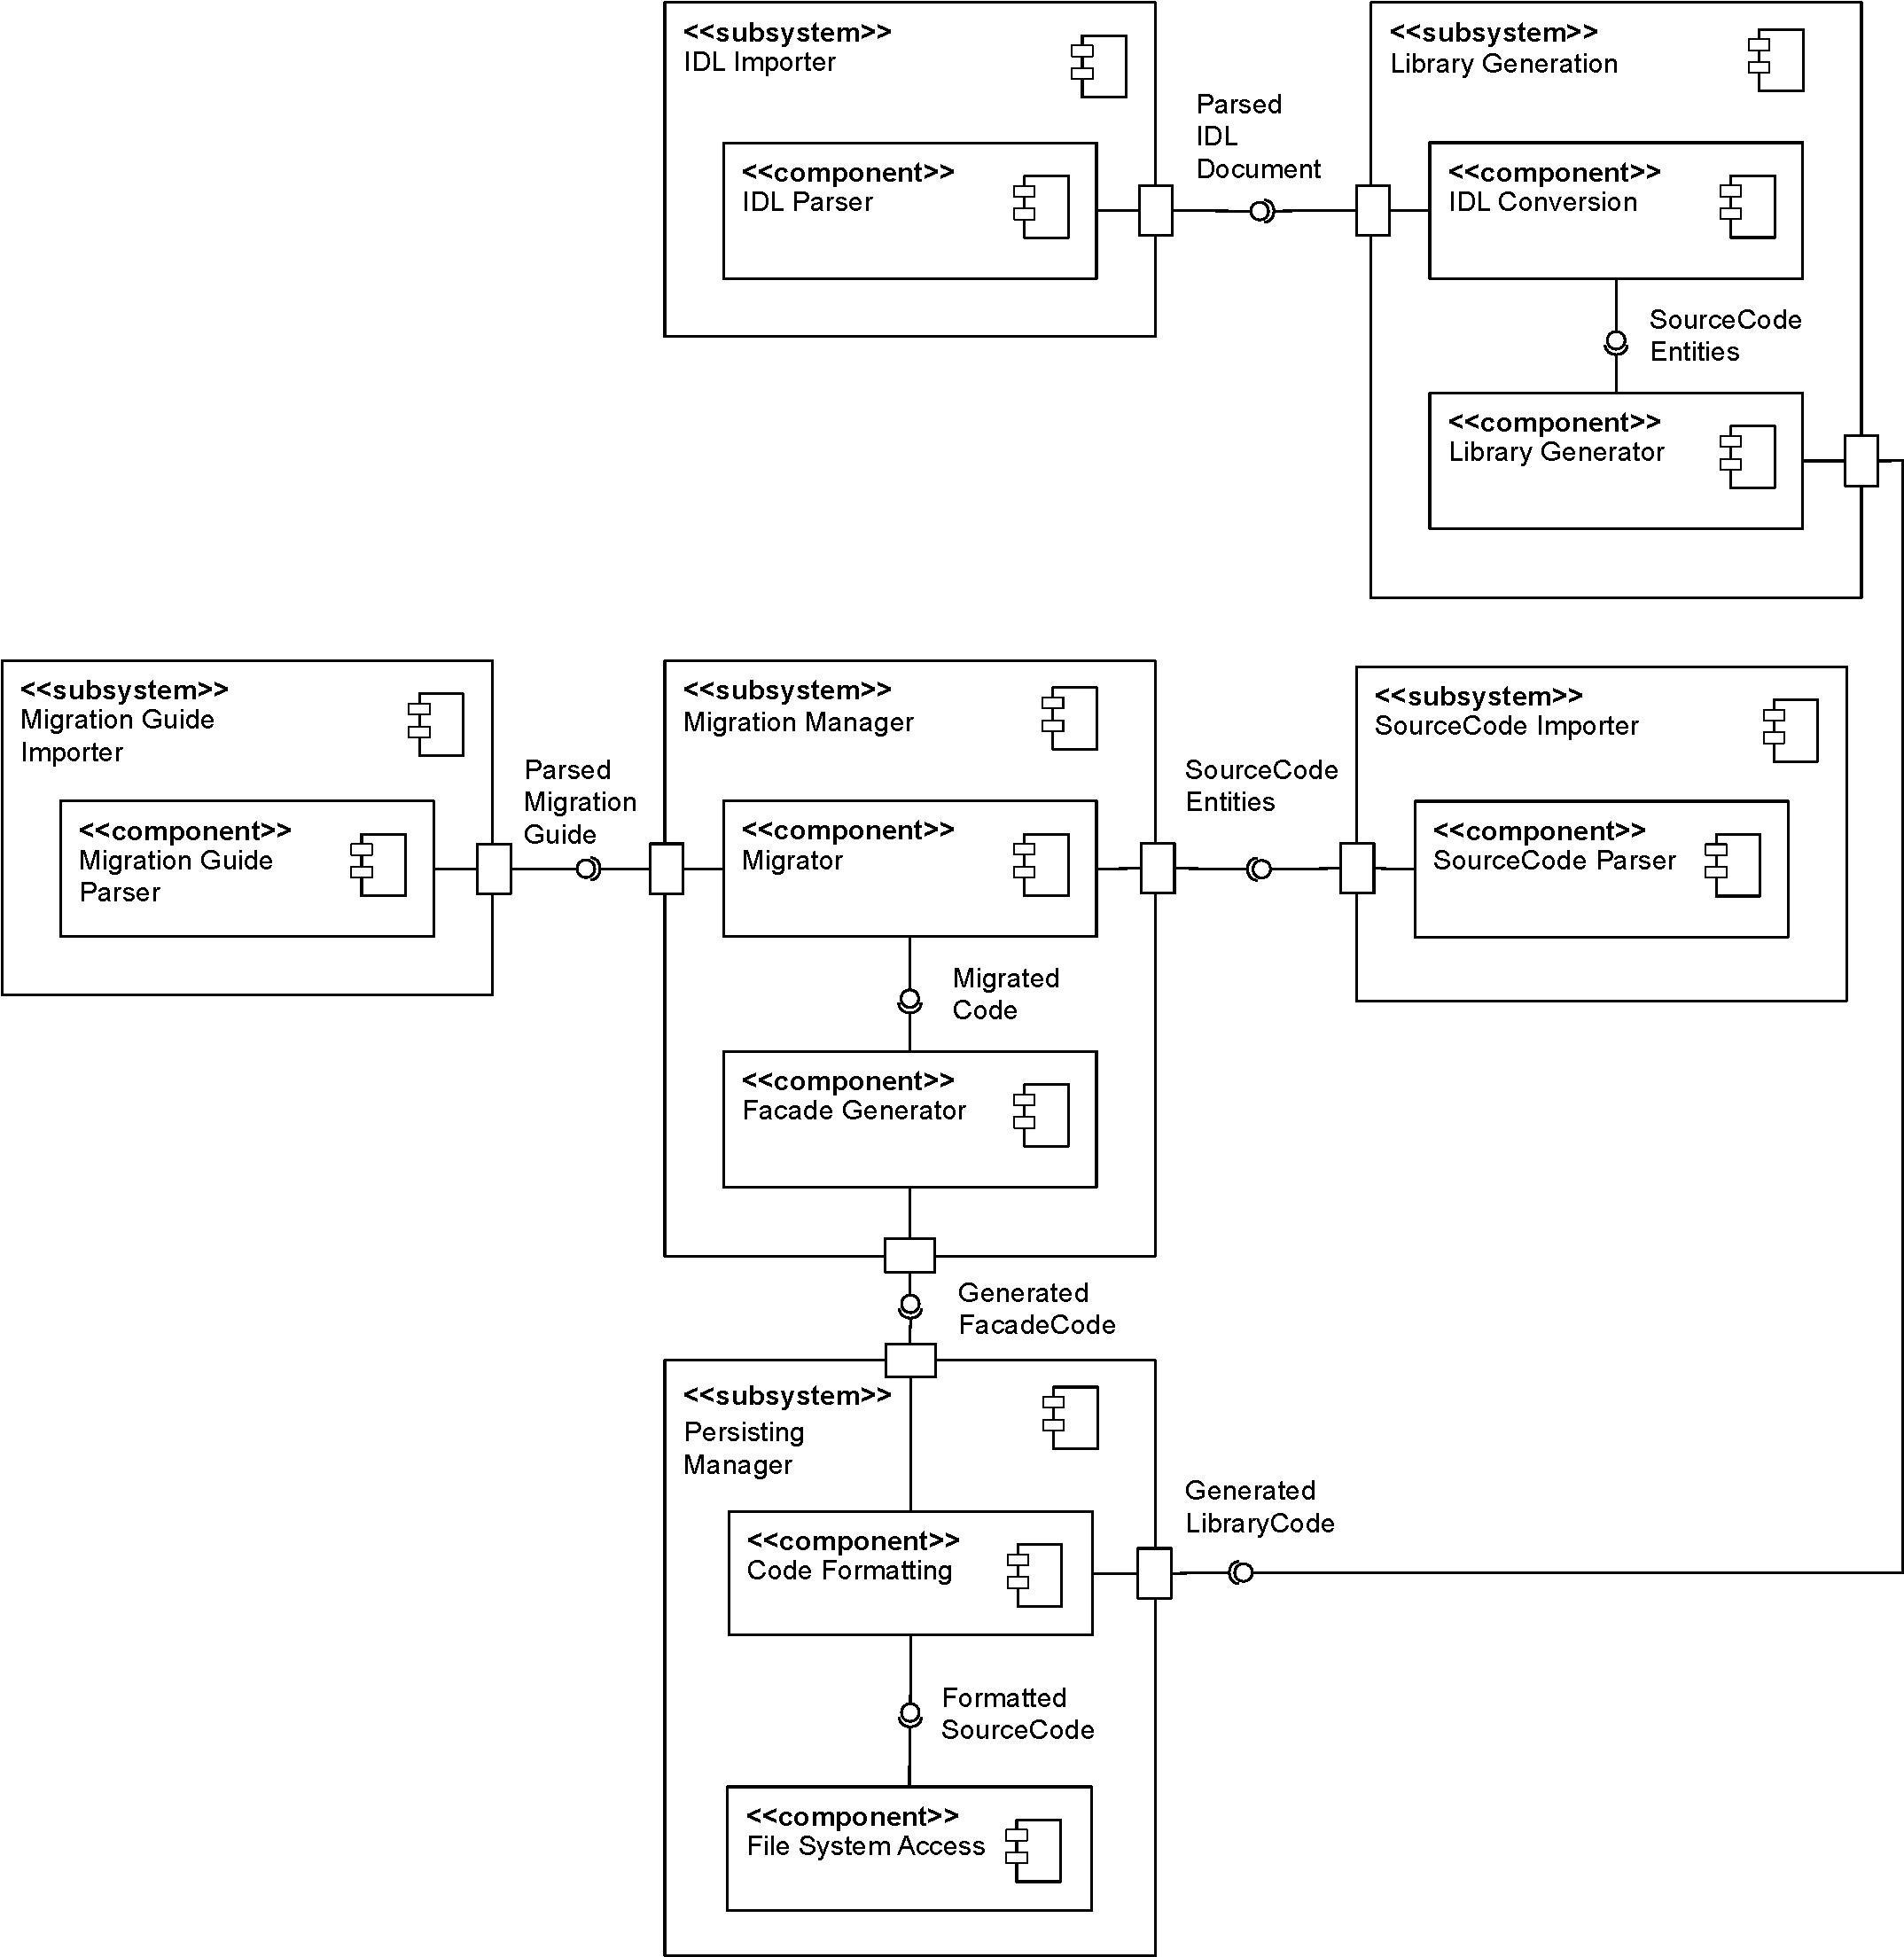
\includegraphics[width=155mm]{images/subsystem_decomposition.pdf}
		\caption{Subsystem decomposition}
		\label{fig:subsystemDecomposition}
	}
\end{figure}

For creating the library and persistent facade subsystem as shown in Figure \ref{fig:outcome}, various tasks need to be executed in order to generate them from IDL documents, previous versions of them and a machine-readable migration guide. 

In order to generate the library subsystem an IDL document must be imported and converted into the source code of a specific programming language. Therefore, a dedicated \texttt{IDL} \texttt{Importer} subsystem for reading and parsing of an IDL document supplies its encoded representation to the \texttt{Library} \texttt{Generation} subsystem. This converts the encoded IDL document into a textual representation of source code of a selected programming language. 

Creating the persistent facade subsystem requires the interaction of several resources that have to be imported first. Our migration guide as shown in Figure \ref{fig:migGuide} includes any changes made to the Web API between the previous and current versions. The corresponding \texttt{Migration} \texttt{Guide} \texttt{Importer} subsystem handles all of the tasks related to fetching, parsing, and validating a migration guide. It provides the parsed representation of the document to the \texttt{Migration} subsystem. For some types of changes, missing information is too cumbersome to be defined in a migration guide and cannot be implicitly derived from an IDL document. Therefore, the source code of the previous version of the facade subsystem must be analyzed to obtain this information. The \texttt{SourceCode} \texttt{Importer} subsystem reads and parses all files of the previous facade and library to provide the encoded result to the \texttt{Migration} subsystem. The \texttt{Migrator} component uses the received information to adapt the previous version of the facade using the changes as stated in the migration guide. Its output is used by the \texttt{Facade} \texttt{Generator} component to generate a textual representation of source code in the desired programming language. 

The emitted source code from both subsystems, \texttt{Migration} and \texttt{Library} \texttt{Gen\-er\-a\-tion}, is used by the \texttt{Persisting} \texttt{Manager} subsystem which formats the code according to a user-defined linting rule set. The formatted source code is written to file using the \texttt{File} \texttt{System} \texttt{Access} component.



\section{Boundary Conditions}
\label{sec:BoundaryConditions}

When using our proposed system, various boundary conditions regarding integration and execution must be taken into account. It is designed to be integrated into an existing CI/CD pipeline of a client application but can also be run locally via a CLI. When it is used as a step in an existing CI/CD pipeline, it must be part of a stage prior to releasing in order to ensure that the most recent version of the Web API is used. Client developers must specify multiple configuration parameters to setup the system. While configuring a migration strategy and specifying a target programming language are mandatory tasks, users can optionally define a linting rule set which determines the code formatting of the emitted code. 

On its initial run, our proposed system does not require a migration guide as the latest version of the Web API is used as a starting point for generating the persistent facade. Hence, only the \ac{URI} of the IDL document needs to be present. After that, each run requires specifying the \acp{URI} of both, the IDL document and the migration guide in order to adapt the facade and update the library subsystems. Omitting mandatory parameters results in an error message during runtime that highlights the missing configuration. Optional parameters do not trigger error messages as a default configuration is used instead. Detecting missing configuration parameters and specifying error messages are tasks of the \texttt{Executable} subsystem.

In addition to configuration parameters, unmet preconditions also raise errors. If the system fails to fetch either the IDL document or the migration guide, no output can be generated and execution will be aborted. The specific reason for the failure is given in the CI/CD system's log or on the command line. Furthermore, if changes specified in the migration guide are incompatible or inconsistent, the facade adaptation will fail and an error message will be logged. Removing a parameter from a non-parameterized method or adding and removing the same parameter to and from a method at the same time are examples of incompatible or inconsistent changes, respectively. Errors related to fetching and parsing of an IDL document or migration guide are managed by the \texttt{IDL} \texttt{Importer} subsystem and \texttt{Migration} \texttt{Guide} \texttt{Importer} subsystem. Checking for incompatibilities and inconsistencies within the migration guide is done by the \texttt{Migrator} component.




\section{Hardware-Software Mapping}
\label{sec:HardwareSoftwareMapping}

For better understanding, in this section the abstract components as shown in Figure \ref{fig:subsystemDecomposition} are mapped to concrete components in an exemplatory execution environment. Therefore, the target client environment is defined as the Apple ecosystem, particularly the development of iOS, iPadOS or macOS-based client applications.  A common use case for this environment is the integration of resource-based Web APIs in the REST architectural style that are described by the OpenAPI \ac{IDL}. Swift is used as the target programming language in which to output the result and to import previous versions of the facade code. By restricting to these criteria, the subsystem decomposition now contains more specific components as shown in Figure \ref{fig:subsystemConcrete}. 

\begin{figure}[!h]
	\centering{
		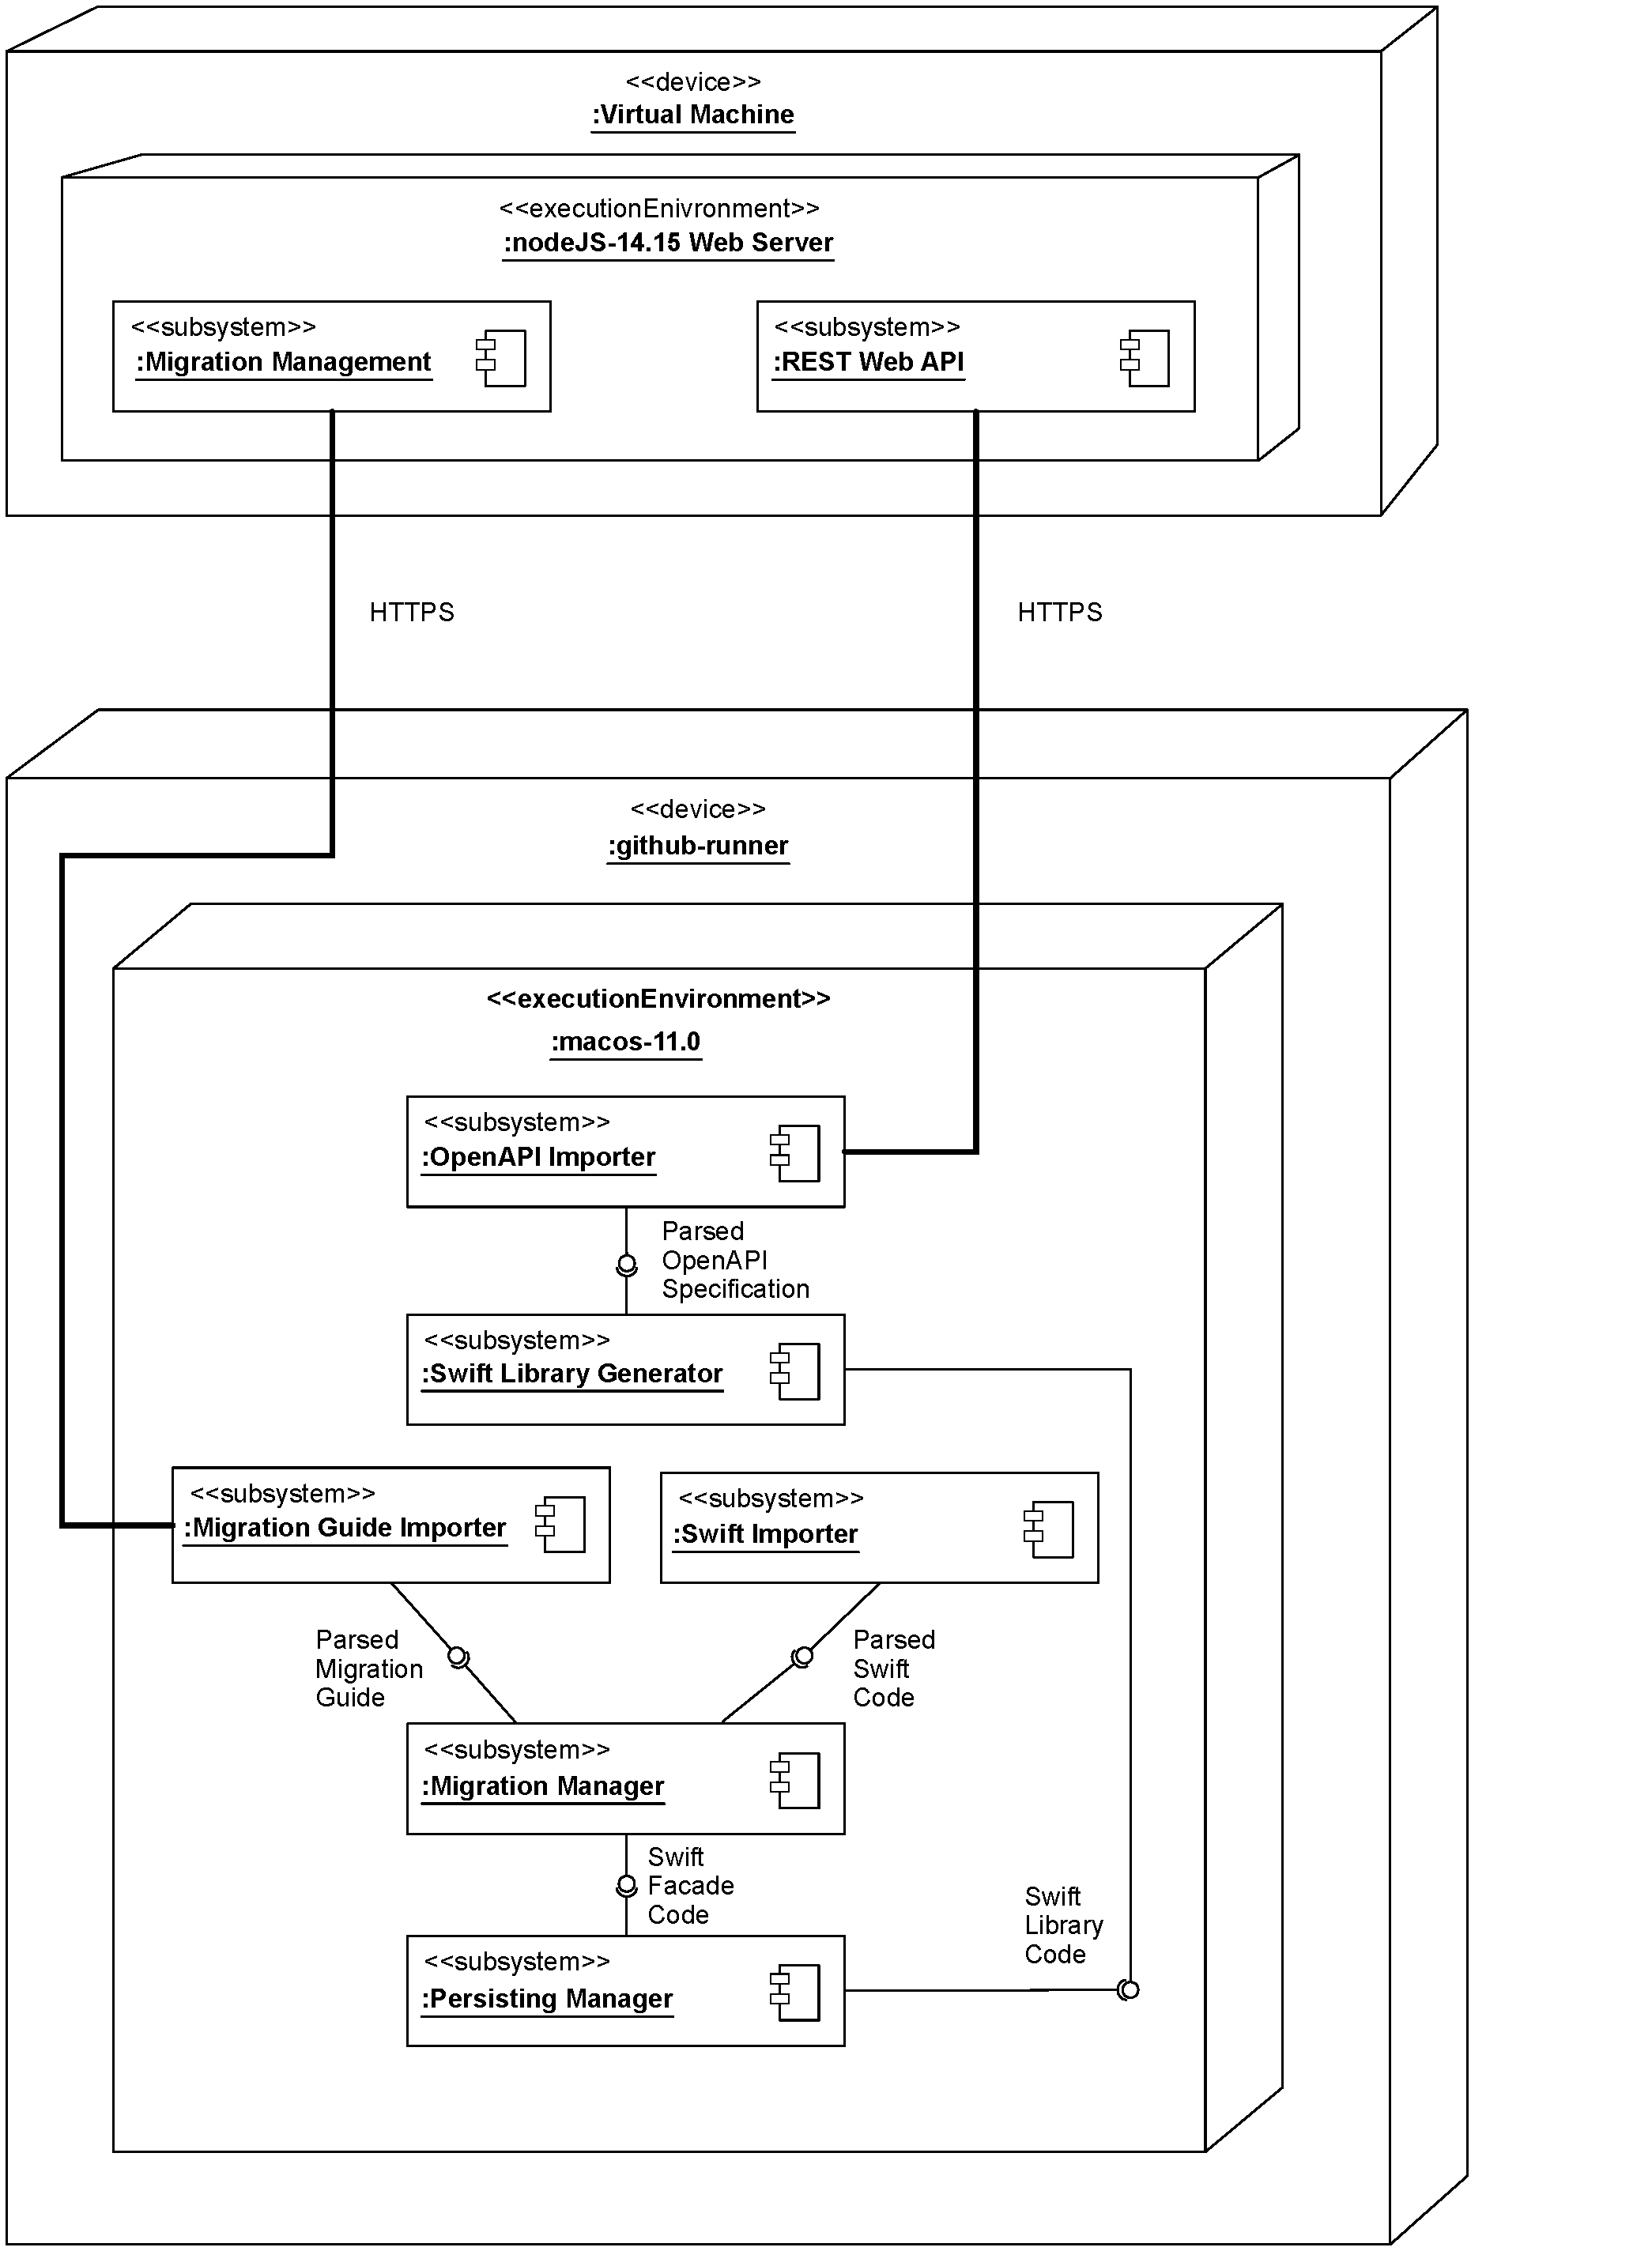
\includegraphics[width=150mm]{images/subsystem_concrete.pdf}
		\caption{Subsystem decomposition in an Apple ecosystem}
		\label{fig:subsystemConcrete}
	}
\end{figure}

The Web API is built using the \ac{REST} architectural style. It is served by a \texttt{nodeJS} web server hosted on a virtual machine maintained by the Web API provider. Its functionality is described using the OpenAPI \ac{IDL}. This document is published on a separate URI of the Web API. Additionally, a \texttt{Migration Management} subsystem is used to track all changes that have been introduced to the Web API. It notes all changes in a machine-readable migration guide and publishes it on a separate URI. Both document can be retrieved using \texttt{HTTPS}. 

To import the specification document, the OpenAPI Importer subsystem must be able to parse specifications using both, the \textit{\ac{JSON}} and \textit{\ac{YAML}} documentation styles. While the system itself can be implemented using an arbitrary programming language, every subsystem that is concerned with importing or generating source code must support Swift. The \texttt{Swift} \texttt{Library} \texttt{Gen\-er\-ation} subsystem uses the parsed specification to create Swift files containing model and endpoint definitions that enable the interaction with the Web API. Appropriate tooling to generate a library from an OpenAPI specification is available for all major programming languages. The OpenAPI Generator\footnote{https://openapi-generator.tech/}, implemented using Java, is one of them, supporting 65 programming languages and dialects. It combines the functionality of the \texttt{OpenAPI} \texttt{Importer} and \texttt{Swift} \texttt{Library} \texttt{Gen\-er\-ation} subsystems.

Parsing a migration guide requires a custom implementation of the \texttt{Migration} \texttt{Guide} \texttt{Importer} as no reusable components exist yet. The subsystem responsible for importing the previous facade must support parsing Swift code. The internal behavior of it is modified according to the changes as stated in the encoded migration guide. After that, the adapted facade is transformed into the textual representation of Swift-based source code by the \texttt{Swift} \texttt{Facade} \texttt{Generator}. There are multiple tools available that support generating Swift code using Stencil templates. The most popular ones are SwiftGen\footnote{https://github.com/SwiftGen/SwiftGen} and Sourcery\footnote{https://github.com/krzysztofzablocki/Sourcery}. They provide similar features that enable users to generate Swift code based on several template types by executing the compiled application via CLI. Sourcery additionally offers a well-maintained framework to enable an integration into existing Swift applications.

The \texttt{Persisting} \texttt{Manager} subsystem uses a linting ruleset to format the library and facade code according to its configuration, before adding meta-files and creating a Swift package which can be imported by client applications using the \textit{\ac{SPM}}. Formatting code based on a linting ruleset is one feature of SwiftLint\footnote{https://github.com/realm/SwiftLint}, the most popular linter for Swift code. While it can be installed and used via CLI, it also supports an integration as a Swift package that enables developers to lint and format Swift code stored in its textual representation.

\chapter{Object Design}
\label{ch:ObjectDesign}

\textit{tbd..}

\newpage
\section{Reuse}
\label{sec:Reuse}

 Software reuse increases the productivity of development teams and improves the overall quality of the product. Therefore, our proposed system defines several components that can be reused from existing solutions. All external components must be open-sourced under the MIT license in order to fulfill our non-functional requirement \ref{nfr:Legal}. Furthermore, custom components of subsystems can be implemented by reusing pattern solutions as defined by the \ac{GoF}. 
 
 Tooling to parse an IDL specification and generate library code for various programming languages is available for many modern Web APIs. For REST-based Web APIs, the OpenAPI Generator\footnote{https://openapi-generator.tech/} is an open-source tool that can be integrated in existing Java projects via Maven/Gradle plugins, or used via CLI and an online service\footnote{http://api.openapi-generator.tech/index.html}. It supports parsing of OpenAPI IDLs regardless of whether they were encoded to YAML or JSON. Additionally, it generates library code in 65 programming languages and dialects. Google's gRPC\footnote{https://grpc.io/} technology uses protocol buffers as an IDL and as a format for exchanging messages. Parsing protocol buffers and generating library code is currently available for 16 programming languages and dialects, with support for additional languages upcoming. Emerging GraphQL\footnote{https://graphql.org/} APIs are described by the \ac{SDL} for which different tools exist that are able to generate library code from it. On the one hand, the GraphQL code generator\footnote{https://graphql-code-generator.com/} supports five programming languages and offers several configuration options to further customize the emitted code. Quicktype\footnote{https://quicktype.io/}, on the other hand, supports 19 programming languages and similar configuration options. One limitation of all tools above is their integrability as a framework. They are designed to generate library code persisted in files, which prevents developers from accessing intermediate artifacts like the decoded IDL document. Generating source code in a programming language that is not supported by those tools requires forking the codebase to extend their functionality. However, for some IDLs and programming languages new frameworks are published that can be integrated into existing projects to get access to intermediate artifacts. For example, the OpenAPIKit\footnote{https://github.com/mattpolzin/OpenAPIKit} is an open-source project that offers a Swift library to en-/decode OpenAPI IDL documents. By separating the parsing of an IDL document and the subsequent library generation, the extensibility for new programming languages and IDL types is considerably increased. 
 
 Supporting multiple programming languages is also a challenge for the \texttt{Source\-Code} \texttt{Importer} subsystem. It must support parsing source code of a programming language into its \ac{AST}. Tools are available for most programming languages as many features of \acp{IDE} like syntax highlighting or auto-completion rely on them. However, most of these tools are commercial products and are not available under an open-source licence. One example is the JavaParser\footnote{https://javaparser.org/} which is available as a Maven and Gradle plugin for parsing, analyzing and generating Java code. Other frameworks were created through the active contribution of open source communities. Acorn\footnote{https://github.com/acornjs/acorn} is a parser for JavaScript code that supports plugins for JavaScript dialects and frameworks like React JSX. Sourcery\footnote{https://github.com/krzysztofzablocki/Sourcery} is a Swift library that provides an \ac{API} that offers parsing and generating Swift code based on Stencil templates. All of these frameworks are limited to parsing source code of a single programming language. To support many different languages simultaneously, custom lexers and parsers must be specified and implemented for each language. While this is a cumbersome manual effort, tools like \ac{ANTLR}\footnote{https://www.antlr.org/} enable developers to generate lexers and parsers in Java, C\#, C++, JavaScript, Python, Swift and Go. Therefore, users have to provide a grammar of the language that describes its structure. This grammar is defined using the Antlr4 grammar syntax. The application's repository contains over 200 predefined grammars that cover many modern programming languages.
 
 Our system uses a machine-readable migration guide to collect all changes that were introduced between subsequent versions of a Web API. In order to fulfill \ref{nfr:MigGuideFormat}, it should be using a \ac{DSL} that is in a human-readable format which is prevalent in the context of web development. While an implementation in a custom language using the auxiliary features of ANTLR would be conceivable, we advocate the use of \ac{JSON} as an external, compositional DSL. This decision is based on the fact that JSON is not just easy to understand and learn, but is also an established standard that is widely adopted by web developers. Another key advantage comes from existing utility libraries for parsing JSON documents in many programming languages. As they are either part of core libraries or can be integrated using third-party open source frameworks, the need to use a custom built lexer and parser is eliminated. Listing \ref{lst:exampleGuide} shows an example JSON-based migration guide that contains one change and specifies some meta-information.
 
 \vspace{2mm}
 \begin{lstlisting}[language=json, caption={Examplatory migration guide in JSON format}, captionpos=b, label={lst:exampleGuide}]
 	{
 		"summary" : "This is an examplatory migration guide.",
 		"api-spec": "OpenAPI",
 		"from-version" : "0.0.1b",
 		"to-version" : "0.0.2",
 		"changes" : [
	 		{
	 			"reason": "Default value was added.",
	 			"object" : {
	 				"operation-id" : "findPetsByStatus",
	 				"defined-in" : "/pet"
	 			},
	 			"target" : "Content-Body",
	 			"added" : [
		 			{
		 				"name" : "_",
		 				"type" : "Pet",
		 				"default-value" : "{ 'type' : 'Cat', age: 2 }"
		 			}
	 			]
	 		}
 		]
 	}
 \end{lstlisting}
 
The decoded representation of a migration guide is used by the \texttt{Migration} \texttt{Manager} subsystem to adapt previous facade code to the changes it contains. Although there are no off-the-shelf components that can be reused, patterns have been identified that are applicaple here. The behavior of the \texttt{Migration} component depends solely on the changes in the migration guide. Therefore, an alternative computational model is to be preferred in contrast to the common imperative models, in which code is organized in an object-oriented manner \cite{fowler_domain-specific_2011}. Fowler et. al coined the term \textit{Semantic Model} to define models that are populated by a \ac{DSL}.  The authors further define an \textit{Adaptive Model} as a specific variation of a Semantic Model in that they take the primary behavioral role in a system. According to the authors, Adaptive Models enable developers to shift the execution context from compile time to runtime and thus change behavior of a running system without a recompile. As the defined behavior is implicit, their implementation is difficult to understand and maintain \cite{fowler_domain-specific_2011}. The ability to alter the migration behavior during runtime by specifying changes in an external migration guide outweighs the negative aspects of using this pattern to model the \texttt{Migration} component. 

Before the generated source code emitted by the \texttt{Library} \texttt{Generation} and \texttt{Facade} \texttt{Generation} subsystems is persisted, users are able to specify formatting rules in order to fulfill \ref{nfr:CodeStyle}. Therefore, multiple open source tools have been created for every modern programming language. SwiftFormat\footnote{https://github.com/apple/swift-format} is an open source tool that formats Swift code using a predefined ruleset. It can be used either via \ac{CLI} or by integrating its framework into an existing Swift application. Prettier\footnote{https://prettier.io/} is a code formatter for multiple languages and dialects used in web development. It supports formatting of JavaScript, JSX, TypeScript and more. Additionally, its active community provides plugins for even more languages like Java, Swift and Ruby. Prettier can be integrated in \acp{IDE} or CI environments and provides an \ac{API} to be used within JavaScript applications. 

All subsystem that deal with importing or generating different types of programming languages or IDL documents are required to adapt their behavior based on the needs of the user. User preferences are provided by configuration options and need to be applied during runtime. The \textit{Strategy} pattern \cite{gamma_design_1995} is a behavioral design pattern that enables selecting these preferences without the need to recompile the application \cite{bruegge_object-oriented_2010}. In our proposed system we identified four subsystems that benefit from applying this pattern.

As shown in Figure \ref{fig:outcome}, our system emits library code that distinguishes between different layers that serve their own purpose. The library layer issues requests and receives responses directly from the Web API. It offers an interface to the facade layer that adapt to changes within the library layer without altering its own public interface. Client applications are unaware of the internal behavior of the facade layer and the interfaces of the library layer. The \textit{Facade} pattern \cite{gamma_design_1995} used here is a software design pattern that enables masking of internal behavior and any changes made to it.
 
\section{Interface Specification}
\label{sec:InterfaceSpecification}

Reusable components and pattern used to create custom components offer their functionality via public-facing interfaces. A detailed specification of these interfaces is required to enable an integration of all subsystems. Additionally, each subsystem defines artifacts that they produce for and consume from other components. The following section demonstrates the internal structure of custom components while for reused third-party subsystems their integration and emitted artifacts are illustrated.

\begin{figure}[!h]
	\centering{
		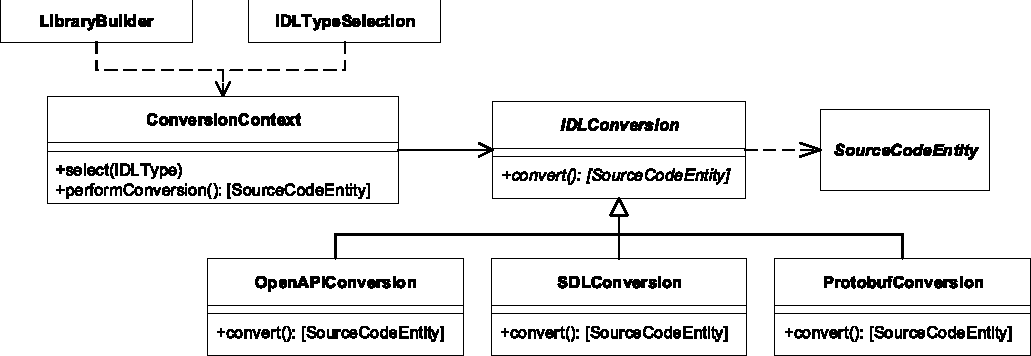
\includegraphics[width=150mm]{images/cd_idl_import.pdf}
		\caption{Class diagram of IDL importer subsystem}
		\label{fig:cdIDLImport}
	}
\end{figure}

Importing an \ac{IDL} for a specific type of Web API needs to flexibly switch between different implementations for various kinds of \acp{IDL}. Therefore, the strategy pattern is used to abstract the internal implementation from the consuming client code. The \texttt{LibraryBuilder} is the client that uses the \texttt{performConversion} method. Depending on the type of IDL which was set by the \texttt{IDL\-Type\-Selec\-tion} for the \texttt{ConversionContext}, the appropriate implementation of \texttt{IDL\-Con\-ver\-sion} performs the conversion and returns a list of \texttt{SourceCodeEntity} objects. 

\begin{figure}[!h]
	\centering{
		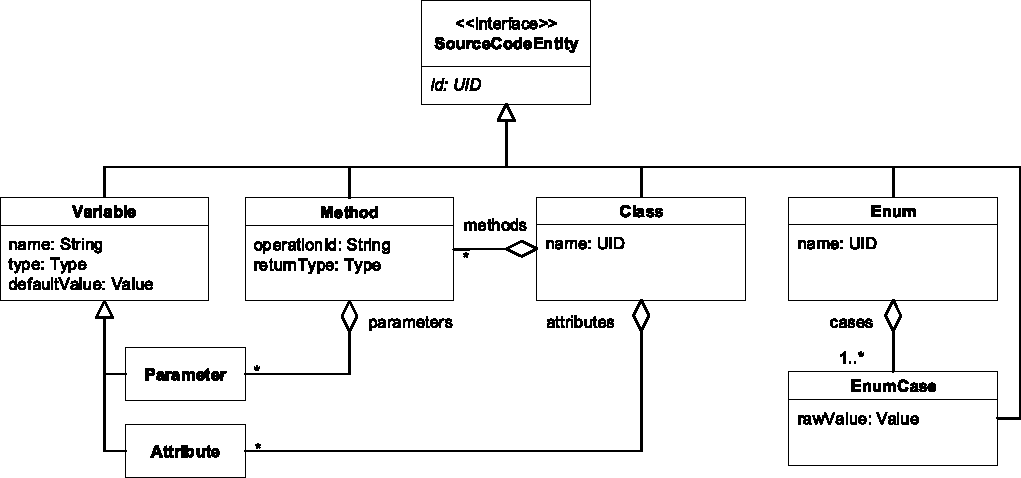
\includegraphics[width=150mm]{images/cd_sourceentity.pdf}
		\caption{Class diagram of source code entity artifact}
		\label{fig:cdSourceCodeEntity}
	}
\end{figure}

\texttt{SourceCodeEntity} objects are used by multiple components. They represent the basic syntactical elements that are common in all modern programming languages. Figure \ref{fig:cdSourceCodeEntity} shows their composition and their most important attributes and relations. \texttt{Class}, \texttt{Method} and \texttt{Enum} entities represent structual elements in which other elements can be nested. A \texttt{Class} element contains \texttt{Attributes} and \texttt{Methods}, whereas \texttt{Enums} specify at least one \texttt{EnumCases}. Each \texttt{Source\-Code\-Entity} can be identified by a \ac{UID}. For \texttt{Class} and \texttt{Enum} elements, their name itself is unique, while for \texttt{Variables}, \texttt{Methods} and \texttt{EnumCases} their context needs to be taken into account.

\begin{figure}[!h]
	\centering{
		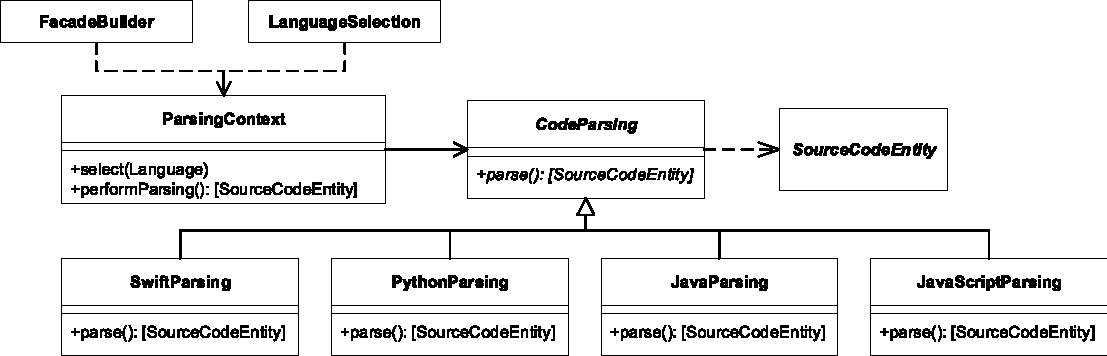
\includegraphics[width=150mm]{images/cd_code_import.pdf}
		\caption{Class diagram of code importer subsystem}
		\label{fig:cdCodeImport}
	}
\end{figure}

Adapting a previous facade to recent changes of a Web API requires importing its source code. Therefore, the \texttt{SourceCode} \texttt{Importer} subsystem must be able to parse source code of multiple programming languages. The decision which programming language needs to be parsed is made during runtime by the user. Since the requirements are the same as those for importing different types of \acp{IDL}, the strategy design pattern is also used here. The selection of the programming language to parse is done by the \texttt{Language\-Selection} component while the \texttt{Facade\-Builder} requests the parsed \texttt{Source\-Code\-Entity} objects.

\begin{figure}[!h]
	\centering{
		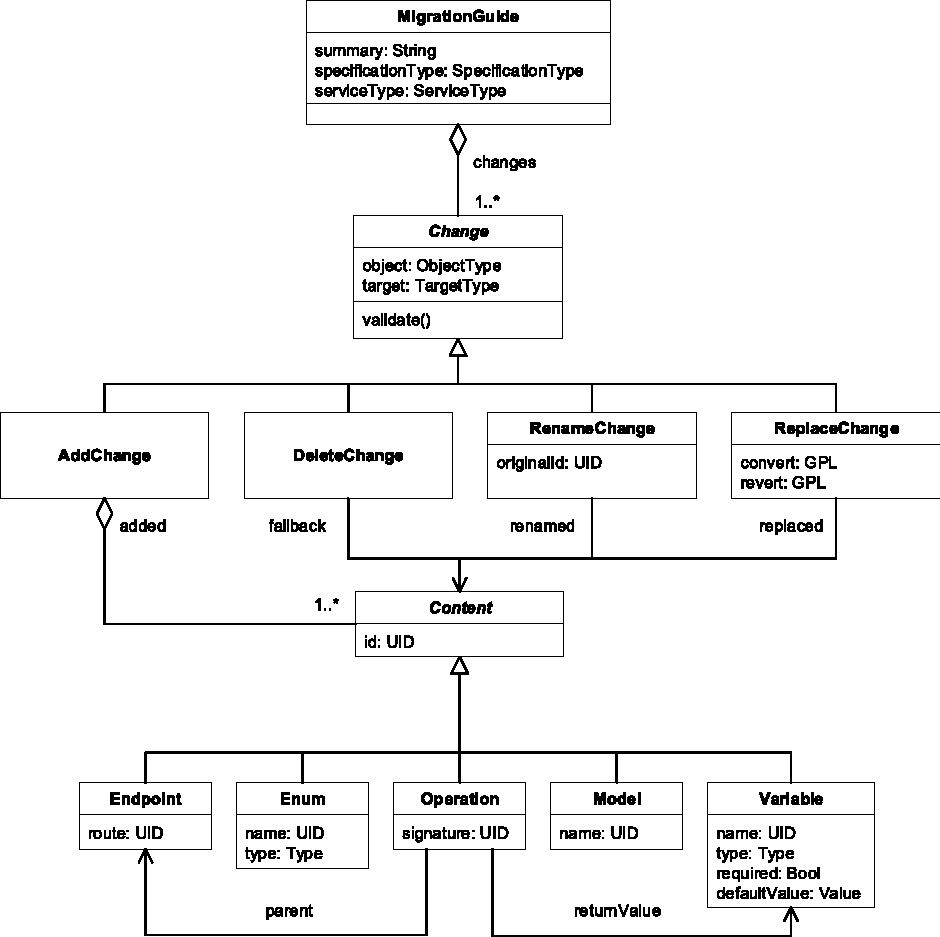
\includegraphics[width=155mm]{images/cd_migguide.pdf}
		\caption{Class diagram of migration guide artifact}
		\label{fig:cdMigrationGuideArtifcat}
	}
\end{figure}

In addition to the decoded representation of the previous facade code, the migration guide needs to be parsed, too. Based on our decision to use \ac{JSON} for defining a migration guide, it can be parsed using a language's core libraries or third-party components. The decoded migration guide structure is shown in Figure \ref{fig:cdMigrationGuideArtifcat}. 

A migration guide contains the type of \ac{IDL} specification in which the Web API is described as well as its service type. Additionally, it specifies all changes that were introduced by the latest version of the Web API. Every change is associated with one of four change types. \texttt{Add\-Changes} denote, that one or more elements of a Web API were added to it. This includes for example adding attributes to a model, parameters to a method or methods to an endpoint. \texttt{Delete\-Changes} indicate that an element was removed from the Web API. For migratable deletions such as removing an attribute of a model, a fallback value can be specified which is used instead of the removed value. \texttt{Rename\-Changes} are used to automate refactorings. Since the functionality of a renamed element remains unchanged, only the previous and new identifications have to be specified here. 

Elements that were renamed and whose functionality also changed are specified with \texttt{Replace\-Changes}. They are the most complex type of change as they need to contain not only the replacement element, but additionally instructions on how to revert them to their previous version and convert their previous to their current version. Code stated in a \texttt{Replace\-Change} needs to be converted into statements of the programming language specified by the user. Instead of introducing another \ac{DSL} or extending the migration guide \ac{DSL}, we decided to use a \ac{GPL} that is common to web developers. We chose JavaScript for that purpose, as it is one of the most used programming language by web developers and it complements \ac{JSON} well. Furthermore, JavaScript code can be directly executed by an interpreter without previously compiling it. Various programming languages support interpreting JavaScript code. For example, Microsoft provides Windows Script Engines\footnote{https://docs.microsoft.com/en-us/previous-versions/windows/internet-explorer/ie-developer/windows-scripting/windows-script-engines} for C\# and Apple released the framework JavaScriptCore\footnote{https://developer.apple.com/documentation/javascriptcore} for Swift and Objective-C in order to parse and interpret JavaScript at runtime .

Each type of change is applied to one object of the Web API and targets one property of it. For example, adding a parameter to a method results in an \texttt{Add\-Change} for a \texttt{Method} object type with a \texttt{Parameter} target type while renaming a model results in a \texttt{Rename\-Change} for a \texttt{Model} object type with a \texttt{Signature} target type. All changes reference \texttt{Content}, i.e. the unique identification of an element of the Web API including additional information that supports the migration process. Invalid changes are indicated by an incorrect combination of their internal information. They are identified by their validation method which reports any errors to the user.

\begin{figure}[!h]
	\centering{
		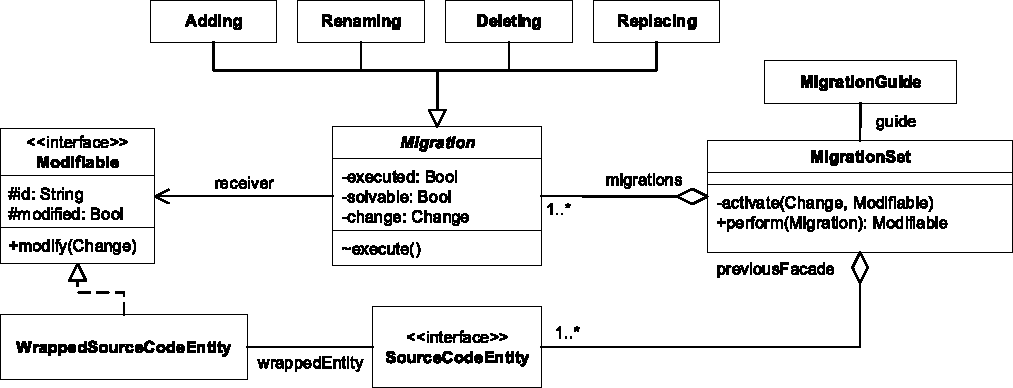
\includegraphics[width=150mm]{images/cd_migration.pdf}
		\caption{Class diagram of migration manager subsystem}
		\label{fig:cdMigrationManager}
	}
\end{figure}

For performing the migration steps, the \texttt{Migration} \texttt{Manager} subsystem incorporates the imported migration guide and decoded previous facade. Analogous to the types of changes corresponding types of migration are defined. \texttt{Migrations} contain the change that must be migrated as well as information that indicates whether they are solvable and have been executed. Furthermore, they reference a \texttt{Modifiable} object on which the migration is performed. The \texttt{Modifiable} interface is implemented by a wrapper component that acts as an adapter for modifying a \texttt{SourceCodeEntity} of the previous facade. By executing a \texttt{Migration}, the \texttt{modify} method of a \texttt{Modifiable} is triggered which adapts the \texttt{SourceCodeEntity} according to the type of migration. The \texttt{mo\-di\-fied} property of a \texttt{Modifiable} denotes that this object has already been migrated. All migrations as well as the previous facade are composed in the \texttt{MigrationSet}. By analyzing the changes stated in the migration guide and their target entities, it creates the corresponding migrations by invoking the \texttt{ac\-ti\-vate} method. Unsupported or incorrect combinations result in an unsolvable migration. The \texttt{MigrationSet} is the public interface of the subsystem by providing the \texttt{perform} method to perform a migration and return the adapted facade element.

\begin{figure}[!h]
	\centering{
		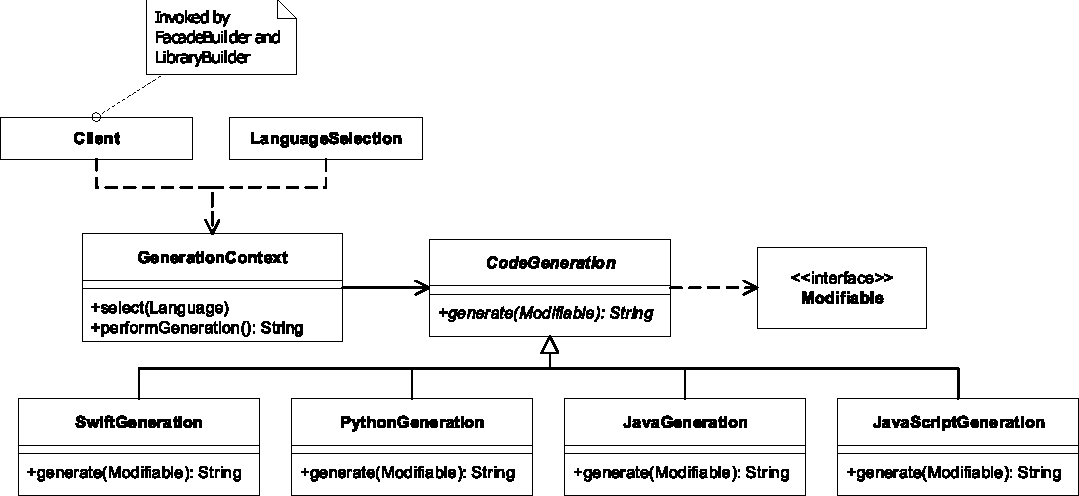
\includegraphics[width=155mm]{images/cd_generation.pdf}
		\caption{Class diagram of code generator subsystem}
		\label{fig:cdGenerator}
	}
\end{figure}

Generating source code from decoded entities for various programming languages requires the \texttt{Code} \texttt{Generator} subsystem to use the strategy pattern. Thereby, the subsystem can select the correct syntax elements during runtime. In contrast to the \texttt{SourceCode} \texttt{Importer} subsystem, it takes wrapped \texttt{SourceCodeEntity} objects as input and generates a string of compilable source code in the programming language the user specified. Its service is used by the subsystems concerned with generating the library code for an IDL and generating the migrated facade code.

\begin{figure}[!h]
	\centering{
		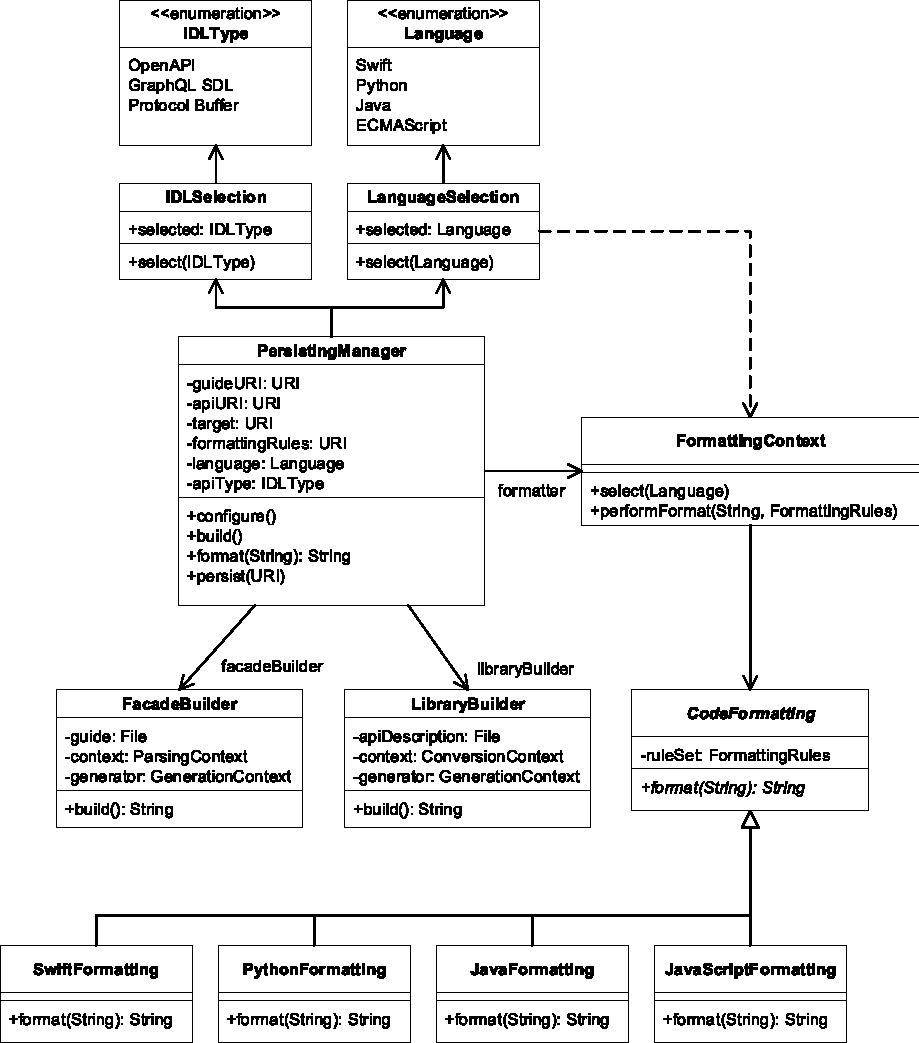
\includegraphics[width=155mm]{images/cd_persisting.pdf}
		\caption{Class diagram of persisting manager subsystem}
		\label{fig:cdPersisting}
	}
\end{figure}

The whole process is orchestrated by the \texttt{Persisting} \texttt{Manager} subsystem. The \texttt{Persisting} \texttt{Manager} takes the user input and selects the desired type of \ac{IDL} and programming language. Additionally, it contains all configuration options of the user that are necessary to retrieve the Web API's \ac{IDL} and migration guide. Furthermore, it contains the ruleset specifying the formatting style of the source code. After configuring the system according to the user's input, the \texttt{build} method starts the importing, adapting and generating process. Therefore, the \texttt{LibraryBuilder} and \texttt{FacadeBuilder} objects are instantiated and their \texttt{build} method is executed. Both objects hold references to their subsystems that are responsible for generating library code from an imported \ac{IDL} and generating source code of an adapted facade, respectively. Once it receives the generated source code strings, the \texttt{PersistingManager} formats the code using a \texttt{Code\-For\-mat\-ting} component instantiated according to the currently selected programming language. As this is done at runtime, the strategy pattern is also applied here. Formatting source code is available by using third-party components for many programming languages, e.g. SwiftFormat\footnote{https://github.com/apple/swift-format} for Swift and Prettier\footnote{https://prettier.io/} for JavaScript und Java. The formatted source code is then persisted by invoking the \texttt{persist} method. Although the internal structure of the emitted library is defined by our system, the user is able to specify its identifier and its target location.
\section{Restructuring}
\label{sec:Restructuring}

After specifying the interfaces of all components, the subsystem decomposition needs to be restructured to reflect all changes. Regarding the generation of code in various programming languages, we identified that the \texttt{Migration} \texttt{Manager} and \texttt{Library} \texttt{Generation} subsystems require the same functionality. As a result, a \texttt{Code} \texttt{Generation} subsystem was extracted that provides its service to the \texttt{Migrator} component and the \texttt{IDL} \texttt{Conversion} subsystem. By that no redundant functionality has to be implemented. 

Additionally, we decided to use JavaScript for handling convert and revert operations defined in \texttt{Replace\-Changes}. Therefore, the \texttt{Source\-Code} \texttt{Importer} subsystem must support parsing it. The restructured subsystem decomposition is illustrated in Figure \ref{fig:subsystemRestructured}.

\begin{figure}[!h]
	\centering{
		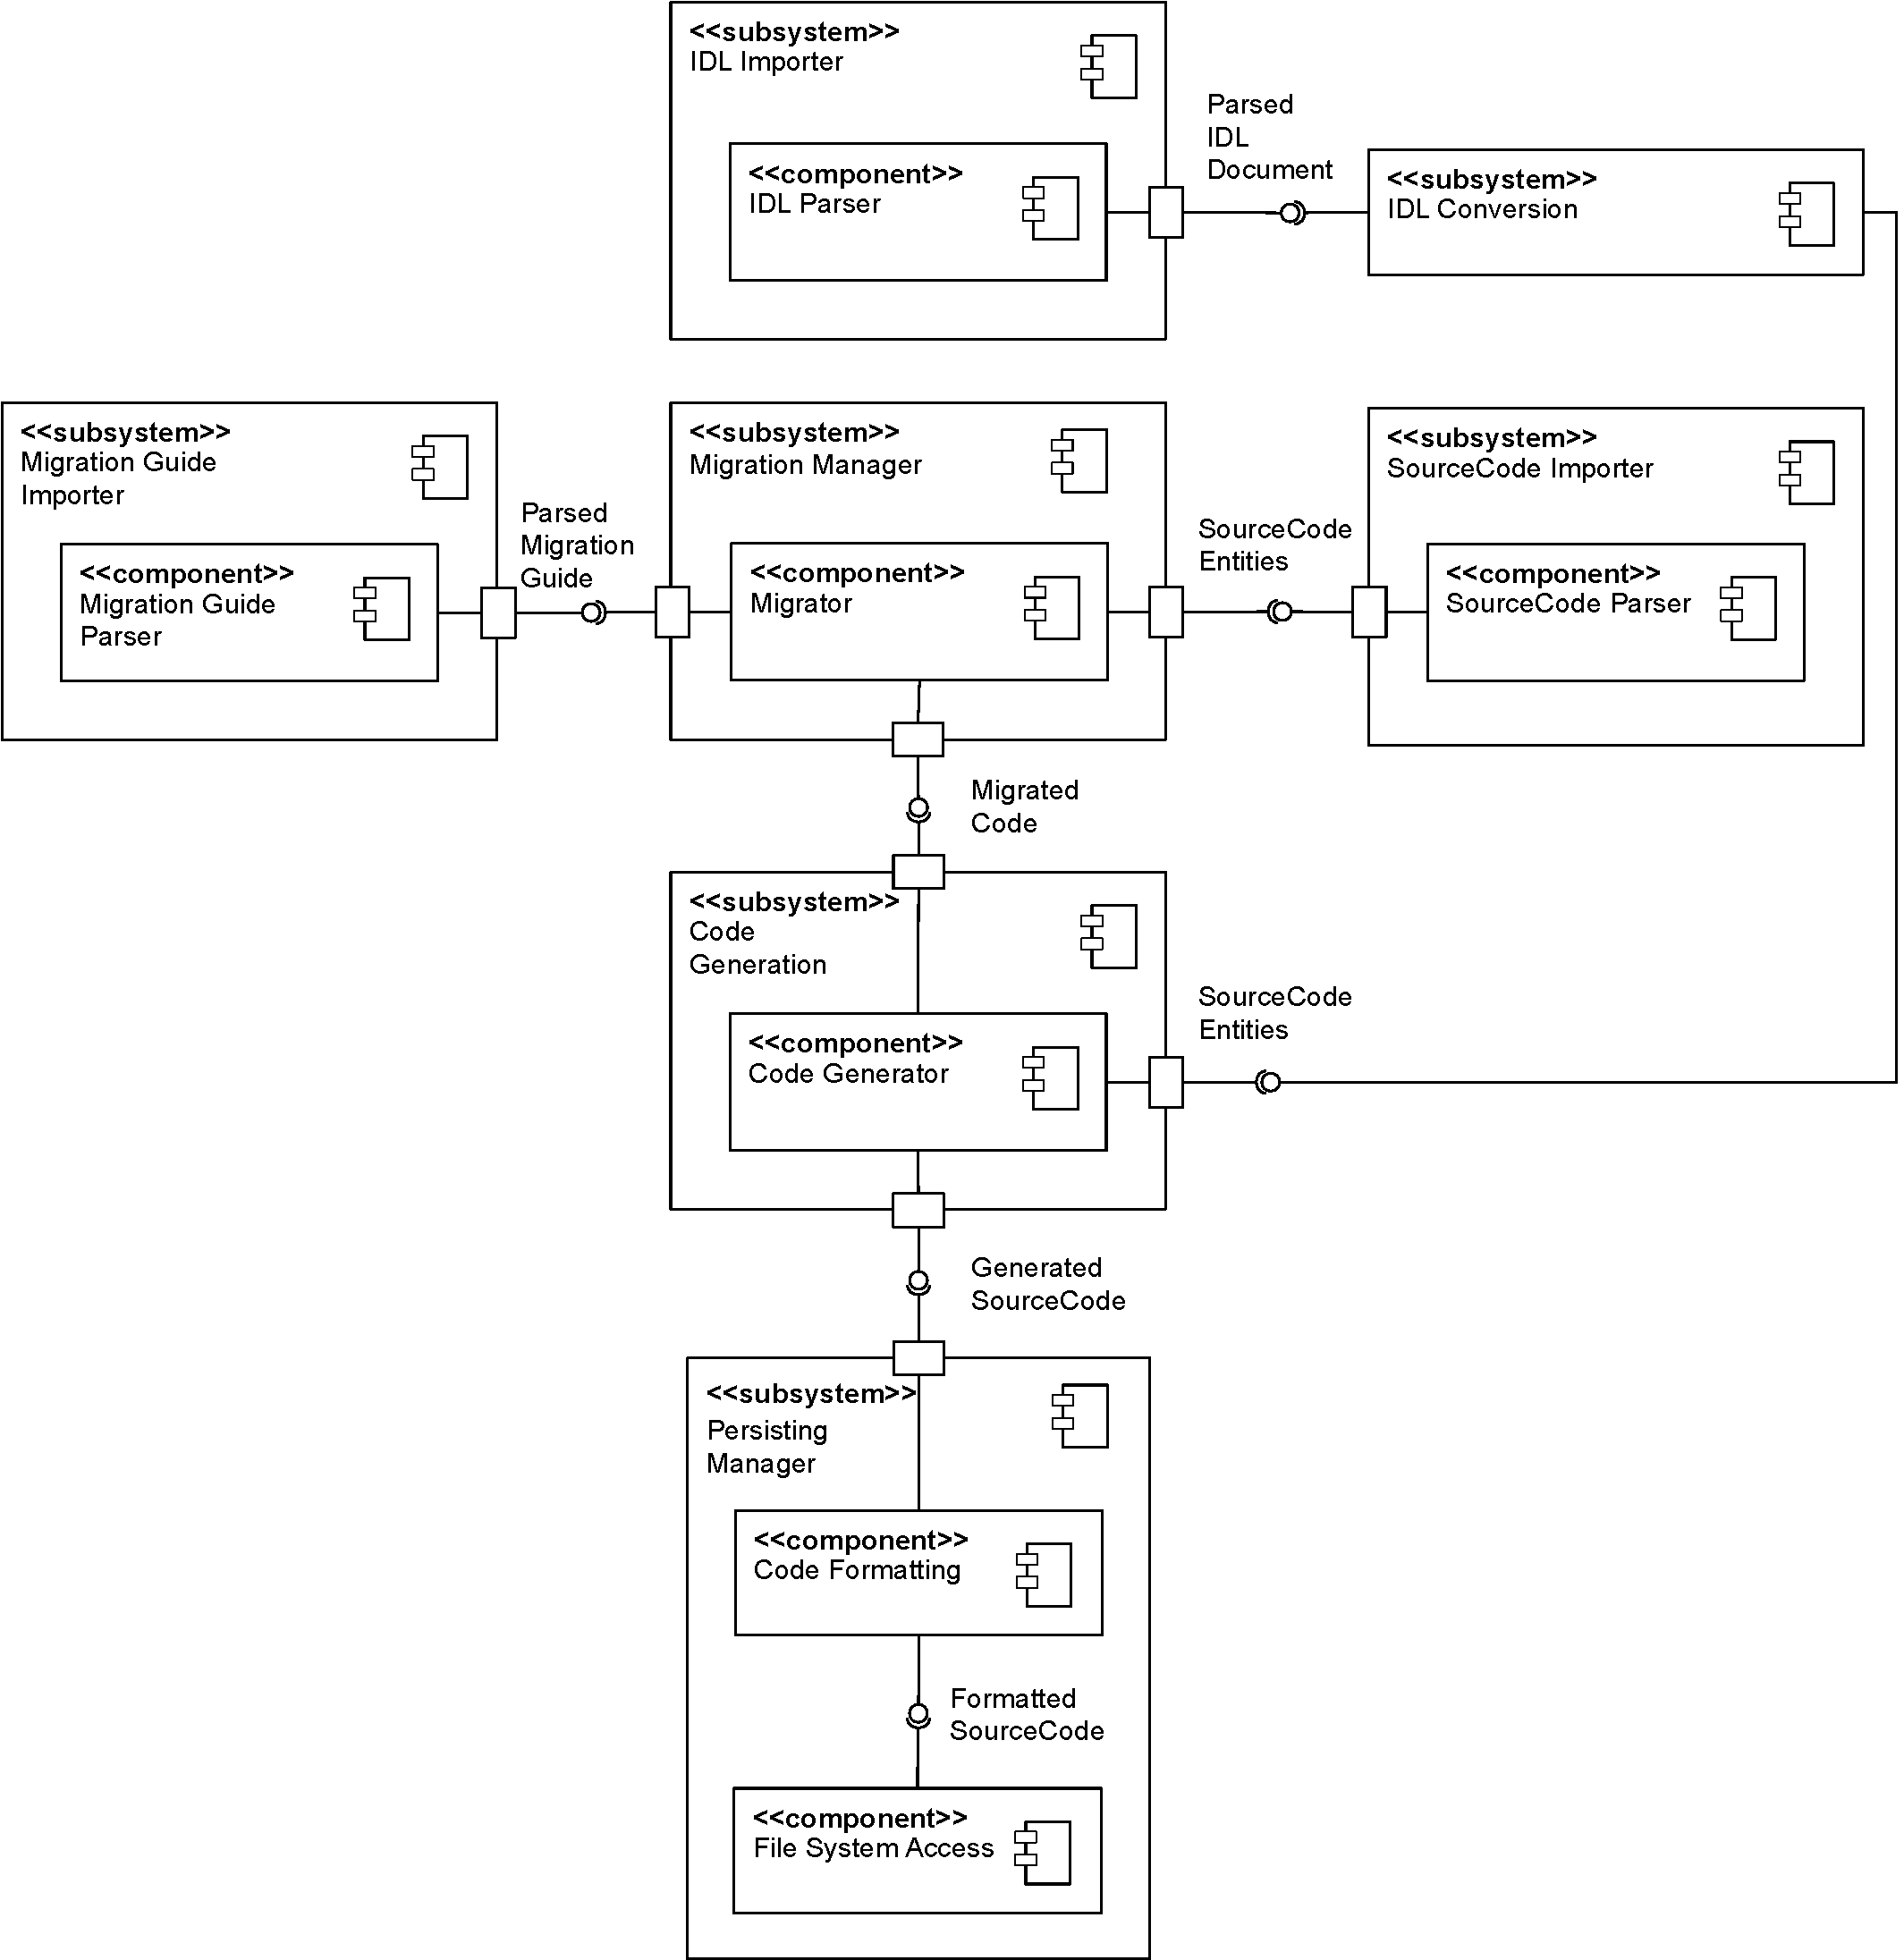
\includegraphics[width=155mm]{images/subsystem_restructured.pdf}
		\caption[Restructured subsystem decomposition]{Restructured subsystem decomposition - The \texttt{Code Generation} subsystem was extracted from the \texttt{Migration Manager} and \texttt{Library Generation} subsystems to provide a uniform interface to both subsystems}
		\label{fig:subsystemRestructured}
	}
\end{figure}
\section{Testing}
\label{sec:Testing}

Testing ensures that all requirements defined in Section \ref{sec:Requirements} and use cases detailed in Section \ref{sec:UseCases} are fulfilled. Therefore, unit tests are specified that test all components of our subsystems in isolation. Furthermore, our integration tests demonstrate the faultless interaction between our subsystems. System tests are defined to ensure that the fully integrated application produces the correct output for various inputs. The testing strategy of our proposed system is subsequently described in a structured manner according to these types of tests.

\paragraph{Unit testing} Unit tests are used to find faults in subsystems with respect to use cases from use case models \cite{bruegge_object-oriented_2010}. Any subsystem for which a custom implementation is preferred over using a third-party component requires extensive testing.

Testing \texttt{UC1}, all subsystems affected by integrating our system are tested in isolation. Various IDL documents must be used as an input for the \texttt{IDL} \texttt{Importer} subsystem which determines their validity and provides the parsed document. While correct IDL specifications are processed without interruption, invalid or incomplete IDL documents raise an error message in the component which is forwarded to the user. Test cases need to be defined for each type of IDL that is supported by the system. For testing the \texttt{IDL} \texttt{Conversion} subsystem, examplatory parsed entites of IDL documents are used to find faults in the conversion algorithm. Its expected output is manually defined and validated based on the emitted source code entities. When the system is set up for the first time, a new facade must be created without migrated changes. Hence, the \texttt{Source\-Code} \texttt{Importer} targets the generated library code in order to create source code entities. Testing this process requires examplatory source code files in various programming languages that are validated based on previously defined source code entities. Empty or invalid files raise a parsing exception. Producing the textual representation of source code needs to be validated by testing the algorithm of the \texttt{Code} \texttt{Generation} subsystem for each supported programming language. Therefore, example collections of source code entities are used as an input that are transformed into strings of source code in the respective language. The unformatted source code strings are formatted by the \texttt{Persisting} \texttt{Manager} subsystem which is tested by validating the formatted source code based on predefined examples. 

\renewcommand{\arraystretch}{1.5}
\begin{table*}[ht]
	\begin{center}
		\begin{tabular}{|>{\raggedright\arraybackslash}m{4cm}|>{\raggedright\arraybackslash}m{5cm}|>{\raggedright\arraybackslash}m{5cm}|}
			\hline
			\begin{center}
				\textbf{Subsystem/ Component}
			\end{center} &  \begin{center}
			\textbf{Input} 
		\end{center}&  \begin{center}
		\textbf{Output}
	\end{center} \\ \hline
			\textit{IDL Importer} & Invalid or incomplete IDL document & Error message \\ \hline
			\textit{IDL Importer} & Valid IDL document & Parsed IDL document \\ \hline
			\textit{IDL Conversion} & Parsed IDL document & Source code entities \\ \hline
			\textit{SourceCode Importer} & Compilable source code  files & Source code entities \\ \hline
			\textit{SourceCode Importer} & Uncompilable source code files & Error message \\ \hline
			\textit{SourceCode Importer} & Source code entities & Unformatted, compilable source code strings  \\ \hline
			\textit{Code Formatting} & Unformatted, compilable source code strings & Formatted source code strings  \\ \hline
		\end{tabular}
		\caption{Input and output of subsystem unit tests for UC1}\label{tbl:UnitTestsUC1}
	\end{center}
\end{table*}

Testing the automated migration is required to detect faults during the upgrade of client source code after the Web API changed (\texttt{UC4}). In addition to the ones defined for \texttt{UC1}, test cases need to be specified that cover importing a machine-readable migration guide and the adaption of the facade to the changes it contains. Since the migration guide is structured using \ac{JSON}, unit tests for the \texttt{Migration} \texttt{Guide} \texttt{Importer} subsystem are performed by the developers of the third-party component. Migrating a previous facade must focus all types of migrations. Additionally, test cases need to be defined for combining different types of changes targeting the same object. Testing this subsystem requires providing example migration guides and manually specified source code entities of a previous facade as an input. Validation is performed by matching the migrated source code entities to predefined end-results. By creating unsolvable \texttt{Migrations}, edge cases can be simulated that result in error messages which need to be forwarded to the user. For example, adding a new parameter to a model of the Web API is unsupported and raises an error message. The message contains information about the type of change, the target object, and a reason for the fault. Incomplete \texttt{Migrations}, i.e. \texttt{Migrations} that do not contain a change, must not be created and result in an unsolvable \texttt{Migration}.

\begin{table*}[ht]
	\begin{center}
		\begin{tabular}{|>{\raggedright\arraybackslash}m{4cm}|>{\raggedright\arraybackslash}m{5cm}|>{\raggedright\arraybackslash}m{5cm}|}
			\hline
			\begin{center}
				\textbf{Subsystem/ Component}
			\end{center} &  \begin{center}
				\textbf{Input} 
			\end{center}&  \begin{center}
				\textbf{Output}
			\end{center} \\ \hline
			\multirow{2}{*}{\textit{Migration Manager}} & Parsed migration guide with changes of multiple target objects & \multirow{2}{5cm}{Migrated source code entities}  \\
			& Source code entities &  \\ \hline
						\multirow{2}{*}{\textit{Migration Manager}} & Parsed migration guide with multiple changes of a single target object & \multirow{2}{5cm}{Migrated source code entities}  \\
			& Source code entities &  \\ \hline
						\multirow{2}{*}{\textit{Migration Manager}} & Parsed migration guide with invalid changes & \multirow{2}{5cm}{Unsolvable Migration object}  \\
			& Source code entities &  \\ \hline
		\end{tabular}
		\caption{Additional input and output of subsystem unit tests for UC4}\label{tbl:UnitTestsUC4}
	\end{center}
\end{table*}

\paragraph{Integration testing} The subsequent tests are used to find faults by testing individual components in combination \cite{bruegge_object-oriented_2010}. Therefore, the public interfaces of the individual components are used to provide the input for the consuming components. Integration tests must be specified for all subsystems, including subsystems that use third-party components.

Identifying faults in the process of generating library code from an \ac{IDL} document requires testing the \texttt{IDL} \texttt{Importer}, \texttt{Library} \texttt{Generation} and \texttt{Code} \texttt{Generation} subsystems. Various \ac{IDL} documents are provided as an input. The results are validated by comparing the generated source code with predefined test examples in multiple programming languages. IDL documents of different types that describe the same Web API must produce the same source code, depending on the programming language. 

For testing the migration process, the interaction of the \texttt{Migration} \texttt{Guide} \texttt{Im\-por\-ter}, \texttt{Migration} \texttt{Manager}, \texttt{Source\-Code} \texttt{Importer} and \texttt{Code} \texttt{Ge\-ne\-ra\-tion} subsystems must be analyzed. Source code files of an examplatory facade and a corresponding migration guide file are mandatory inputs. For identifying any faults, predefined examples for multiple programming languages are compared against the generated output. By combining different changes, some of them targeting the same object, errors caused by contradicting or incompatible information can be detected. 

\begin{table*}[ht]
	\begin{center}
		\begin{tabular}{|>{\raggedright\arraybackslash}m{4cm}|>{\raggedright\arraybackslash}m{5cm}|>{\raggedright\arraybackslash}m{5cm}|}
			\hline
			\begin{center}
				\textbf{Subsystem/ Component}
			\end{center} &  \begin{center}
				\textbf{Input} 
			\end{center}&  \begin{center}
				\textbf{Output}
			\end{center} \\ \hline
			\textit{IDL Importer} & \multirow{3}{5cm}{Valid IDL document} & \multirow{3}{5cm}{Unformatted, compilable source code strings}   \\
			 \textit{Library Generation} &  &  \\
			 \textit{Code Generation} &  &  \\ \hline
			 			\textit{Migration Guide Importer} & Compilable source code files & \multirow{4}{5cm}{Unformatted, compilable source code strings}   \\
			 \textit{Migration Manager} & Migration guide with multiple changes of multiple target objects &  \\
			 \textit{SourceCode Importer} & \multirow{2}{*}{}  &  \\
			 \textit{Code Generation} &  &  \\ \hline
		\end{tabular}
		\caption{Input and output of subsystem integration tests}\label{tbl:IntegrationTests}
	\end{center}
\end{table*}


\paragraph{System testing} System testing tests all the components together, seen as a single system to identify faults regarding functionality, performance issues and user related problems \cite{bruegge_object-oriented_2010}. 

For testing the systems functionality, its command line interface is used to set different configuration options and produce a library for accessing a Web API. The system works as defined if the emitted code compiles and is able to communicate with the Web API. Error messages issued by the Web API, e.g. in the event of unauthorized access, do not represent a system failure. When integrated into the CI/CD pipeline of a client application, the system uses a preset configuration to produce the library code every time its stage is executed.

Performance tests ensure, that all nonfunctional requirements and design goals are fulfilled \cite{bruegge_object-oriented_2010}. Missing mandatory configuration parameters must result in error messages displayed by the \ac{CLI}. The system provides a parameter to list all parameters and other helpful advice. Important messages must be colored to clearly emphasize their information. The generated library code must be formatted according to the user's ruleset and contains documentation derived from the \ac{IDL} document. All code emitted in a specific programming language must use the syntax elements of its latest major version.
\chapter{CaseStudy / Evaluation}
\label{ch:CaseStudyEvaluation}

Evaluating our proposed system demonstrates its usefulness in a potential target environment. For the concrete instantiation, the Swift programming language was selected to implement custom subsystems. Required functionality that was already available is integrated using third-party Swift packages. All used packages are published under MIT license. Since it is a prototypical implementation, it supports importing IDLs only for REST-based Web APIs that are described using the OpenAPI specification. Furthermore, its support for generating client libraries is limited to the Swift programming language. 

Section \ref{sec:Implementation} addresses the details of the implementation of \textsc{Pallidor} which is composed of three libraries that are developed and maintained as standalone Swift packages. Each package is described in detail in its respective section, which provides an overview of the package's control flow and public interface. Furthermore, each section details how the package can be integrated into existing applications and shows its current limitations.


For evaluating our proposed system, we perform a migration of two consecutive Web API versions using Pallidor. Therefore, we manually manipulate the Open\-API specification of the sample \texttt{Pet} \texttt{Store}\footnote{https://petstore3.swagger.io/} Web API so that it reflects all change types we identified. Furthermore, we manually create a machine-readable migration guide for each version of the Open\-API specification to document all occuring changes. 

The evaluation in Section \ref{sec:Evaluation} is structured according to the degree of automation to which the respective type of change can be migrated. Changes of the first category, \textsc{Automated Migration}, can be automatically migrated by using Pallidor with our novel machine-readable migration guide. The second category, \textsc{Semi-Automated Migration}, contains changes that can be migrated by Pallidor, but which also require manual intervention by client developers to overcome them. Changes that require new approaches to automating their migration are addressed in the third category, \textsc{Manual Migration}. Each category describes the problems that are caused by the types of change as well as our approach to solving these problems including its benefits and consequences. Each category is concluded by providing our evaluation process and results.

\newpage
\section{Implementation}
\label{sec:Implementation}

For evaluating the proposed system, we created \textit{Pallidor} a prototypical implementation using the Swift programming language. It is composed of multiple subsystems that are developed and maintained as standalone Swift packages. Each package provides the functionality of a subsystem that is defined in Section \ref{ch:SystemDesign}. \texttt{PallidorGenerator} implements the \texttt{IDL Conversion} and \texttt{IDL Importer} subsystems. Migrating a previously generated facade is performed by the \texttt{Pal\-lidor\-Migrator} package that provides the services of the \texttt{Migration Ma\-na\-ger}, \texttt{Migration Guide Importer} and \texttt{SourceCode Importer} subsystems. 

\begin{figure}[!h]
	\centering{
		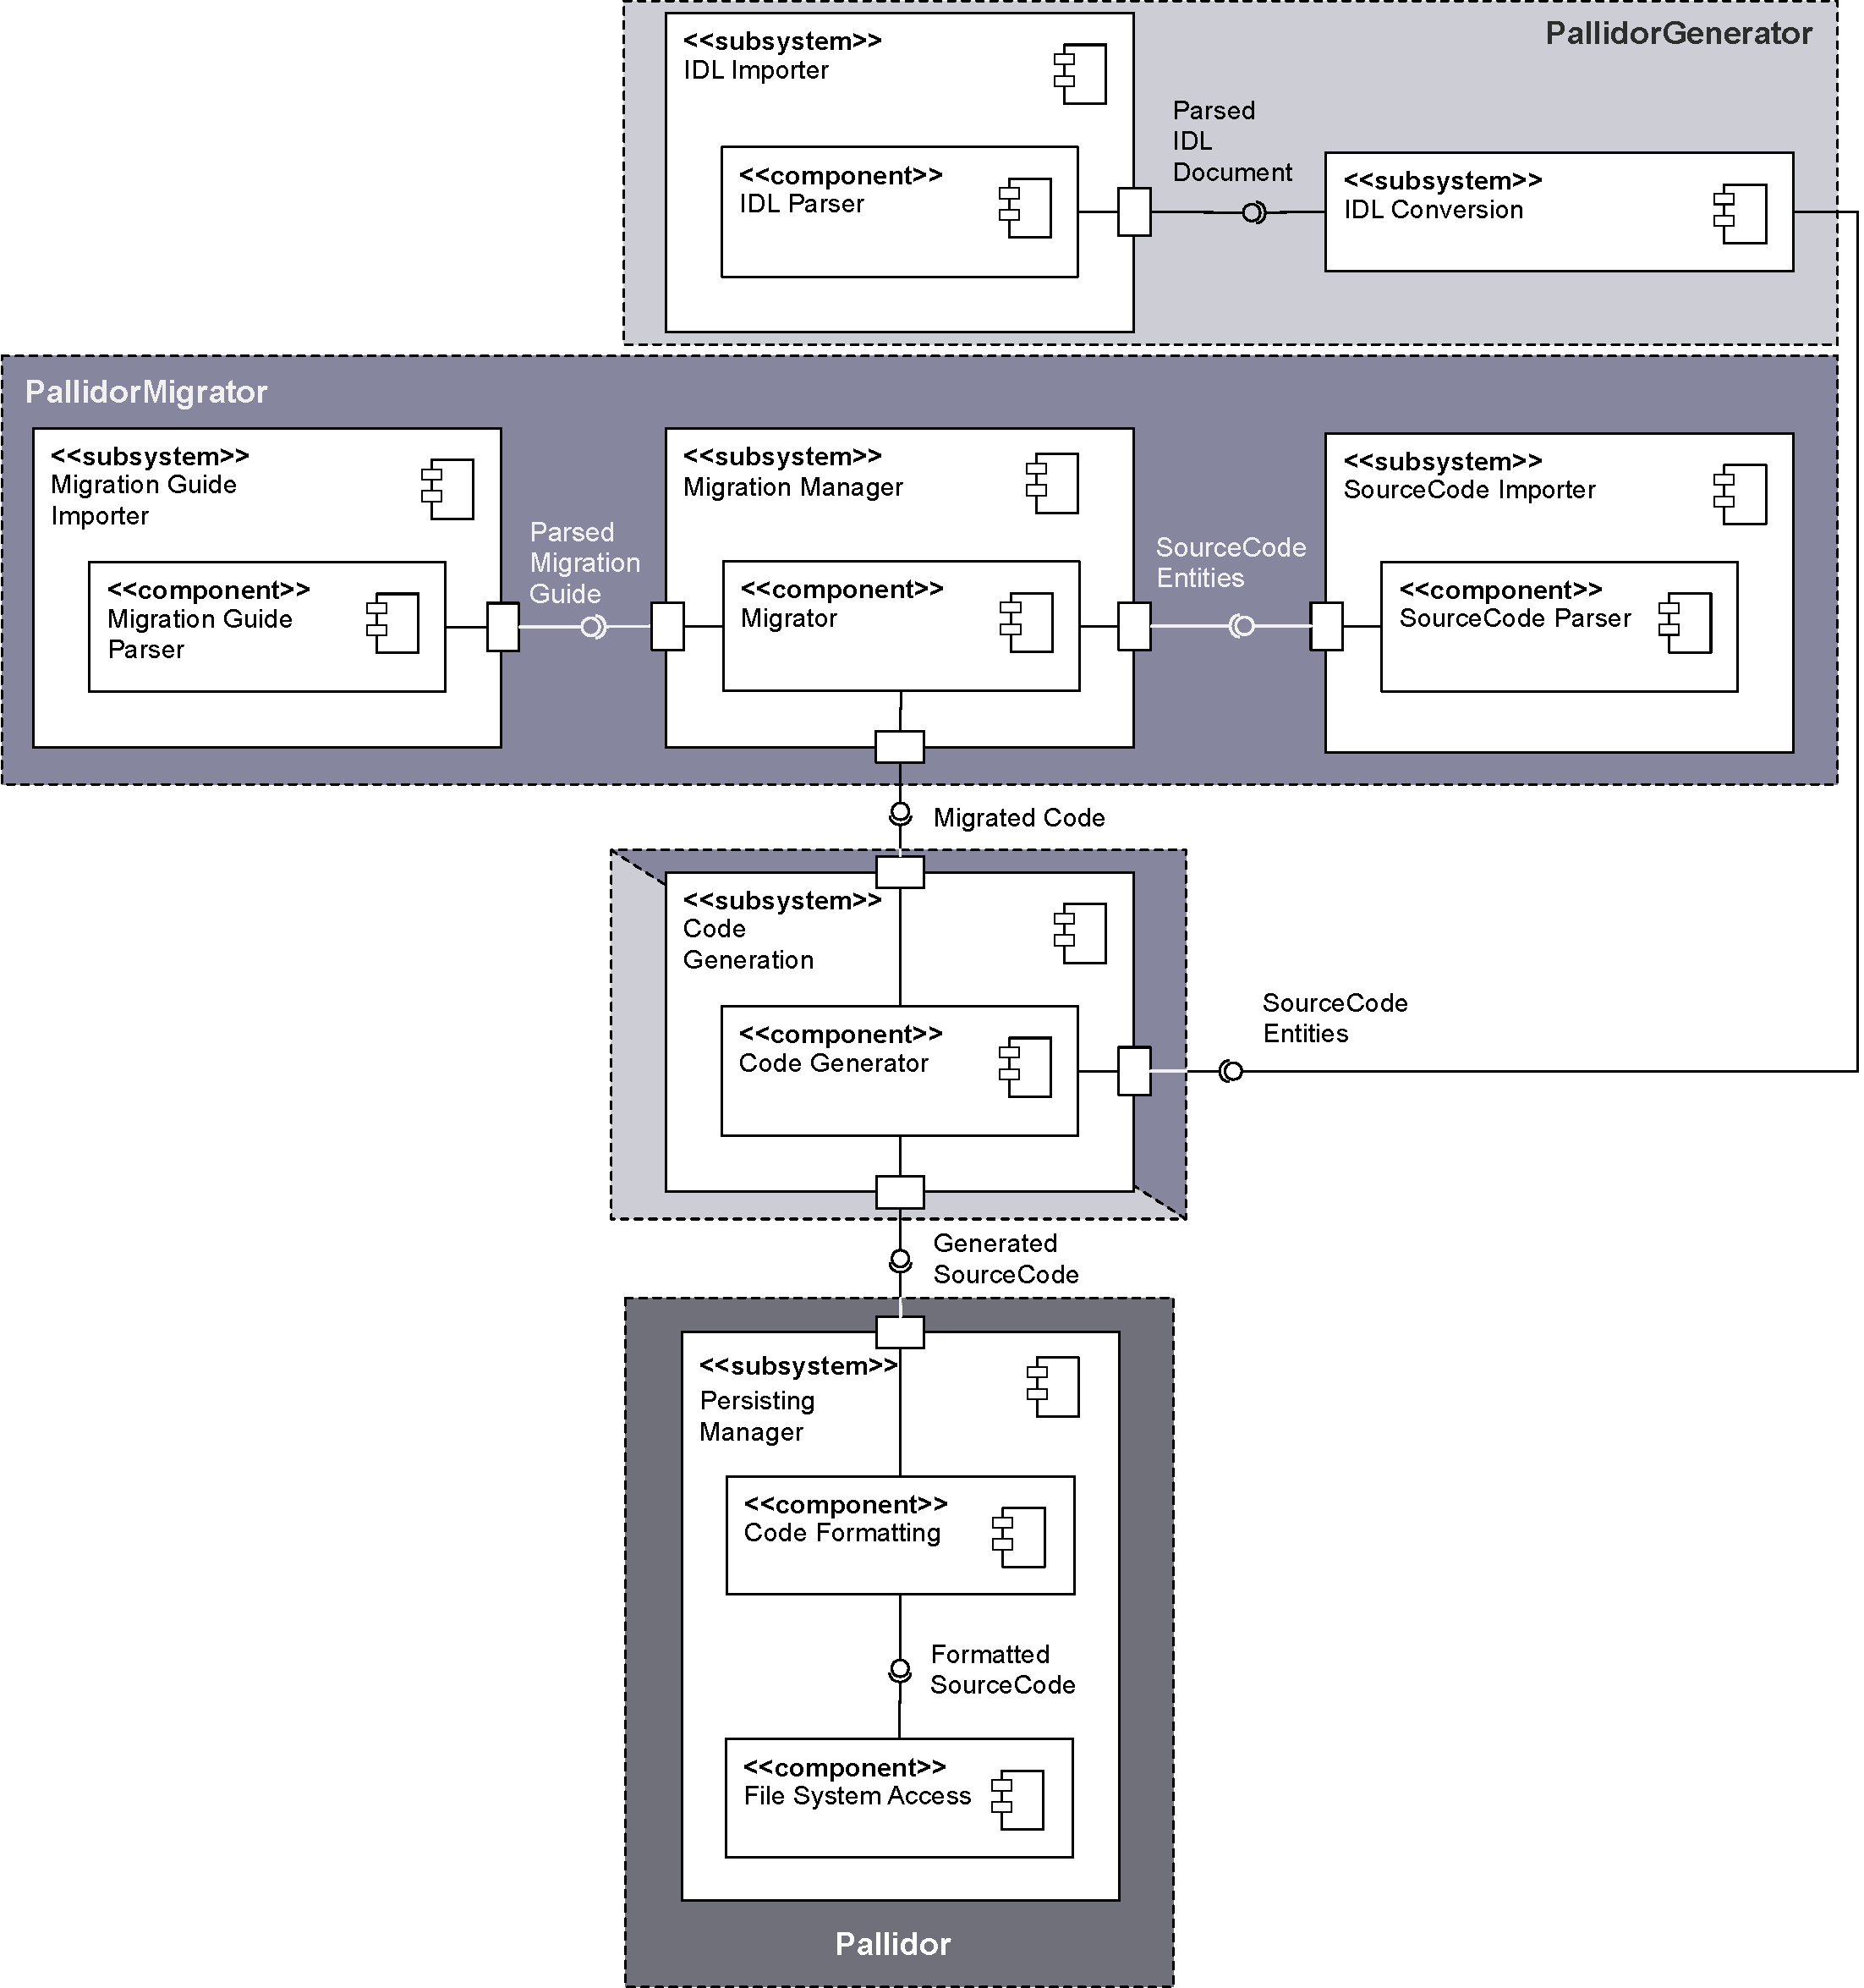
\includegraphics[width=140mm]{images/subsystem_implementation.pdf}
		\caption{Implementation of subsystems with Pallidor Swift packages}
		\label{fig:subsystemImplementation}
	}
\end{figure}
Both packages implement the functionality of the \texttt{Code Generation} subsystem and persist their respective results in files. The \texttt{Code Generation} subsystem is not separately implemented because our prototype only supports the Swift programming language. The \textsc{Pallidor} package combines both subpackages in an executable that provides a command-line user interface. Furthermore, it formats the source code and persists it afterwards. Figure \ref{fig:subsystemImplementation} illustrates which package implements the respective subsystem.  

In addition to our own implementations, third-party open-source components that provide the required functionality are integrated using the Swift Package Manager. Key components and their respective implemented subsystems are listed in Table \ref{tbl:PallidorDep}. Since Pallidor is a prototype, its functionality is limited to generating a persistent Swift package from an OpenAPI specification. It can be integrated in client applications using Swift in version 5.2 or later. Since our generated Swift package uses Apple's \texttt{Combine}\footnote{https://developer.apple.com/documentation/combine} framework, the client application's execution environment must be at least iOS 13 or MacOS 10.15. 

\renewcommand{\arraystretch}{1.4}
\begin{table*}[ht]
	\begin{center}
		\begin{tabular}{|>{\centering\arraybackslash}m{2.7cm}|>{\centering\arraybackslash}m{3cm}|>{\centering\arraybackslash}m{3.2cm}|>{\centering\arraybackslash}m{4cm}|}
			\hline
			\begin{center}
				\textbf{Subsystem/ Component}
			\end{center} &  \begin{center}
				\textbf{Swift Package Name} 
			\end{center}&  \begin{center}
				\textbf{Swift Package Version}
			\end{center} &
		 \begin{center}
			\textbf{Swift Package Author / Publisher}
		\end{center} \\ \hline
			\textit{IDL Importer} & OpenAPIKit & 2.2.0 \newline (Dec. 20th, 2020) &
			Mathew Polzin \\ \hline
			\textit{Source Code Importer} & Sourcery & 1.0.2 \newline (Nov. 30th, 2020) &
			Krzysztof Zabłocki \\ \hline
			\textit{Code Formatter} & swift-format & 0.50300.0 \newline (Sep. 19th, 2020) &
			Apple, Inc. \\ \hline
		\end{tabular}
		\caption{Third-party Swift packages used for subsystems in Pallidor}\label{tbl:PallidorDep}
	\end{center}
\end{table*}

The \texttt{OpenAPIKit} is a library that enables encoding to- and decoding Swift types from OpenAPI documents. It supports importing documents structured in JSON and YAML formats and provides Swift types for most types of the OpenAPI specification in (3.0.2). In its latest version, the \texttt{OpenAPIKit} does not support \texttt{Link Objects} and specification extensions for \texttt{OpenAPI.XML} and \texttt{OpenAPI.Oauth\-Flows}. As opposed to the OpenAPI specification, this library specifies the \texttt{re\-qui\-red} property of schema elements on the element instead of the parent object. OpenAPI documents must be provided as \texttt{Data} or \texttt{String} types, as the \texttt{OpenAPIKit} does not support reading files. Furthermore, all reference elements (\texttt{\$ref}) must be internal references and target the same file in order to be resolved.

\texttt{Sourcery} is a code generator for Swift, built on top of Apple's \texttt{SourceKit}. It extends its functionality and types to facilitate generating Swift code based on Stencil templates. Although \texttt{Sourcery} is designed as a command-line tool to be integrated in a custom build phase, it provides a framework that can be incorporated using the Swift Package Manager. In addition to generating Swift code, it provides support for parsing Swift strings in corresponding source code entities. 

Formatting the generated Swift code is performed by \texttt{swift-format}. It can be used as a command-line tool or integrated into applications using the Swift Package Manager. It provides an API to format Swift code according to a style configuration. If no set of styling rules is specified, a default style is used. The package is compatible with Swift 5.1 and higher and requires selecting the appropriate branch that corresponds to the version of Swift used in the integrating application.

\subsection{Pallidor Generator}\label{subsec:PallidorGenerator}

The \texttt{PallidorGenerator} Swift package is concerned with retrieving and parsing of OpenAPI specifications to generate the library layer of the Swift package for the client application. Therefore, OpenAPI specifications must be parsed and converted to source code entities. After that, they are transformed into source code strings in the Swift programming language and are persisted in files. The package integrates the \texttt{OpenAPIKit} which decodes an OpenAPI specification in its \texttt{Open\-API.Document} type. This type is composed of elements that represent the attributes of an OpenAPI specification. Furthermore, it provides a locally dereferenced representation that facilitates the traversal of its structure by replacing all \texttt{\$ref} elements with their referenced entities. The \texttt{OpenAPI.Document} needs to be converted to source code entities before Swift code can be generated. This conversion is performed during the traversal of the document by using various \texttt{Resolver} objects. Depending on the OpenAPI specification element that needs to be converted, a corresponding \texttt{Resolver} initializes a source code entity model using the information of the OpenAPI element. Resolving an endpoint struct from the \texttt{Resolved\-Route} type of the \texttt{OpenAPIKit} is shown in Listing \ref{lst:Resolving}.

\begin{lstlisting}[language=Swift, caption={Resolving an operation}, captionpos=b, label={lst:Resolving}]
	/// Resolves an endpoint struct
	/// - Parameters:
	///   - path: path in OpenAPI document
	///   - route: Resolved route from OpenAPI document
	/// - Returns: resolved EndpointModel
	static func resolve(path: OpenAPI.Path, route: ResolvedRoute) -> EndpointModel {
		let endpoint = EndpointModel(
				name: path.components[0].upperFirst(), 
				operations: [], 
				detail: route.summary)
		endpoint.operations = route.endpoints.map( 
				{ OperationModel.resolve(endpoint: $0) })
		return endpoint
	}

\end{lstlisting}

All source code entity models of the \texttt{PallidorGenerator} package are extended with the \texttt{Custom\-String\-Convertible} protocol that adds the \texttt{description} computed property. It is used to specify string templates for generating the Swift code of the library layer. They are dynamically composed of all string templates of nested models such as methods, parameters or properties. Furthermore, static templates for meta files such as the \texttt{Package.swift} file are provided as Markdown (\texttt{.md}) files. Although minor adjustments are made, for example specifying the name of the Swift package, their functionality remains the same between different Web APIs.

\begin{lstlisting}[language=Swift, caption={Source code string template for an endpoint}, captionpos=b, label={lst:EndpointTempl}]
	/// Extension of the Endpoint Model
	/// Used for generating client library code in Swift
	extension EndpointModel : CustomStringConvertible {
		var description: String {
			"""
			import Foundation
			import Combine
			
			struct _\(name.upperFirst())API {
				static let decoder ...
				\(operations
				.sorted(by: {$0.operationId < $1.operationId})
				.map({$0.description})
				.joined())
			}
			"""
		}
	}

\end{lstlisting}

The public interface of the \texttt{PallidorGenerator} Swift package is provided by the file of the same name. Its initialization requires specifying the URL of the OpenAPI specification to be decoded. Depending on its format, a \texttt{JSON\-Decoder} or \texttt{YAML\-Decoder} is created that is used to decode the OpenAPI specification. Initializating the \texttt{Pal\-li\-dor\-Gen\-er\-ator} fails, if the OpenAPI document cannot be decoded or resolved due to an invalid URL or malformed structure. Generating the Swift code of the library layer and persisting it in files is performed by invoking its \texttt{generate} method. It receives a \texttt{path} parameter and the name of the client library as specified by the user. After generating all files, a list of their URLs is returned to the method's caller. The method throws an error if writing the files in the target directory fails. Several OpenAPI specifications of various Web APIs are used for testing the \texttt{PallidorGenerator} Swift package. They are specified in Markdown files and are located in the \texttt{Resources} subfolder of the test folder. The generated files are validated against predefined results specified in Markdown files that are located in the \texttt{Results} subfolder. 

Integrating the \texttt{PallidorGenerator} package in a Swift project, the URL of its GitHub repository must be added to the dependencies in the \texttt{Package.swift} file. Furthermore, the \texttt{develop} branch must be selected for using its latest version.
\newpage
\begin{lstlisting}[language=Swift, caption={Integrating PallidorGenerator in SPM}, captionpos=b, label={lst:IntegrationGenerator}]
	.package(
			url: "https://github.com/Apodini/PallidorGenerator.git", 
			.branch("develop")
	)
\end{lstlisting}


With regard to the implementation of the \texttt{PallidorGenerator} Swift package, some restrictions must be observed. Instead of defining inline objects in nested elements of an OpenAPI specification, schema components must be used to specify custom data types. They must be referenced at their designated target element. This limitation is based on the problem that nested elements do not provide an identification, which is required for building the library layer. The Open\-API specification supports defining primitive data types as schema components using a custom name. These type aliases are resolved and their underlying primitive types are used in the generated client library. Furthermore, all endpoint methods in an Open\-API specification must specify the \texttt{operationId} property. Analogous to schema components, this identifier is used by \textsc{Pallidor} to recognize changes and to generate the client library. Although it is not enforced by the OpenAPI specification, all operations must specify at least one response that is returned after the request was processed successfully. Otherwise the return value type of an operation cannot be inferred from the Open\-API document. Unlike successful responses, error responses can be of various types.
\subsection{Pallidor Migrator}\label{subsec:PallidorMigrator}

The \texttt{PallidorMigrator} package integrates the functionality of the \texttt{Migration} \texttt{Ma\-nager}, \texttt{Migration Guide Importer} and \texttt{SourceCode Importer} subsystems. It uses the information stated in the parsed migration guide to adapt the source code entities of a previously generated facade layer. Therefore, a set of migrations is initialized that performs the necessary migratory steps on the changed target properties of the source code entity. After migrating all changes, the source code entities are converted into Swift code that gets persisted in files. The machine-readable migration guide is parsed by the builtin \texttt{JSONDecoder} of Swift's \texttt{Foundation} framework. The \texttt{PallidorMigrator} package provides a model for mapping the migration guide to its decoded representation. Depending on the type of change that is stated in the migration guide, the \texttt{MigrationSet} initializes a corresponding \texttt{Migration} object. Each \texttt{Migration} is checked for plausiblity on its initialization. Thereby, invalid or inconsistent changes are detected and its \texttt{solvable} property is set to false. An unsolvable \texttt{Migration} results in an error message that is propagated to the user. Every \texttt{Migration} targets one source code entity of a previously generated facade. The \texttt{Sourcery} framework is used for importing its source code. It provides source code entities for all syntactical elements of Swift code such as classes, structs and methods. These entities cannot be extended within the \texttt{PallidorMigrator} package, because they are declared as \texttt{final}.

\begin{lstlisting}[language=Swift, caption={Extending a wrapped Sourcery struct}, captionpos=b, label={lst:WrappedStruct}]
	/// Wraps struct types of Sourcery
	class WrappedStruct: Modifiable {
		...
		convenience init(from: SourceryRuntime.Struct) {
			self.init(
				localName: from.localName.removePrefix, 
				variables: from.variables
					.map({ WrappedVariable(from: $0) }), 
				methods: from.methods
					.map({ WrappedMethod(from: $0) }))
		}
	}
\end{lstlisting}

In order to adapt them to changes, wrapper classes are used to extend their functionality with the \texttt{Modifiable} protocol. This protocol introduces a \texttt{modify} method that receives a \texttt{Change} object as a parameter. A modifiable endpoint struct that wraps the \texttt{SourceryRuntime.\-Struct} type of the \texttt{Sourcery} framework is shown in Listing \ref{lst:WrappedStruct}. Depending on the type of change that the \texttt{modify} method receives, the corresponding handling routine is performed. 

\begin{lstlisting}[language=Swift, caption={Modification of a changed method entity}, captionpos=b, label={lst:MethodModify}]
	/// Wrapped method of SourceryMethod
	class WrappedMethod: Modifiable {
		...
		func modify(change: Change) {
			self.modified = true
			switch change.changeType {
				case .add:
					handleAddChange(change: change as! AddChange)
					break
				case .rename:
					handleRenameChange(change: change as! RenameChange)
					break
				case .replace:
					handleReplaceChange(change: change as! ReplaceChange)
					break
				case .delete:
					handleDeleteChange(change: change as! DeleteChange)
					break
			}
		}
	}
\end{lstlisting}

Their implementations vary depending on the type of source code entity that is modified. They adapt an entity's associated properties according to the details of the migration. In Listing \ref{lst:MethodModify}, the implementation of the \texttt{modify} method highlights the various handling routines that are used to migrate the properties of a \texttt{WrappedMethod}. Similar to the source code entities of the \texttt{PallidorGenerator} package, the wrapped source code entities provide templates that are used to convert them into Swift code. These source code strings are persisted in files.

The public interface of the \texttt{PallidorMigrator} Swift package is provided by the file of the same name. Its initialization requires specifying the URL of the migration guide and the URL of the directory in which the previously generated client library is located. If the migration guide cannot be retrieved or decoded, an error message is thrown and forwarded to the user. Furthermore, on initialization of the \texttt{PallidorMigrator} struct a set of migrations is created. If their plausibility check fails, an error message is shown to the user. Migrating the changes as stated in the migration guide and persisting the adapted facade layer in files are started by invoking the \texttt{buildFacade} method. After generating all files, it returns a list of their URLs. An error is thrown if writing the files of the adapted facade layer fails. The \texttt{PallidorMigrator} Swift package is extensively tested to discover erroneousness migrations. Therefore, migration guides are created that contain various types of changes with their respective targets. The unit tests migrate prepared source code entities according to these migration guides and compare the outcome to predefined results. Various integration tests are performed that combine different changes on a single target to ensure that they do not affect each other. The input documents of previously generated facade layer code and their predefined adapted results are specified in Markdown files located in the \texttt{Resources} subfolder of the test folder. 

Integrating the \texttt{PallidorMigrator} package in a Swift project, the URL of its GitHub repository must be added to the dependencies in the \texttt{Package.swift} file. Furthermore, the \texttt{develop} branch must be selected for using its latest version.

\begin{lstlisting}[language=Swift, caption={Integrating PallidorMigrator in SPM}, captionpos=b, label={lst:IntegrationMigrator}]
	.package(
		url: "https://github.com/Apodini/PallidorMigrator.git", 
		.branch("develop")
	)
\end{lstlisting}

The implementation of the \texttt{PallidorMigrator} Swift package deviates from the design of our proposed system. In addition to the original design, the generated library layer must also be imported. No migration guide or previously generated facade can be used during the initial integration of \textsc{Pallidor} as the current version of the Web API is persisted. Therefore, the facade layer is generated based on the public interface of the library layer. Furthermore, no migration strategy can be selected so that all changes of a WebAPI are migrated. A limitation of \texttt{Sourcery} concerns the automatic documentation of the public facade layer of the client library because it does not support parsing comment annotations. Therefore, the documentation for the client library is located at the library layer and must be consulted manually. Additionally, some types of migration must be performed by combining multiple migratory steps. Replacing an endpoint is achieved by replacing all of its methods and then renaming it. Renaming and replacing enum cases and inherited schemas is accomplished by adding their replacements before removing them. Return values of endpoint methods can only be replaced because they do not specify a name that could be renamed. Furthermore, all operations must provide a return value type, which means that deleting them or adding them later is not applicable.
\subsection{Pallidor}\label{subsec:Pallidor}
The \textsc{Pallidor} package contains the command-line user interface and the \texttt{Code\- Formatting} component. Furthermore, it stores all configuration settings of the user. By invoking \textsc{Pallidor} via its commandline interface and providing all required configuration parameters, the client library is generated. The \texttt{swift\-argument-parser}\footnote{https://github.com/apple/swift-argument-parser} package is used to supply detailed error and help messages and it facilitates type-safe argument parsing. The URLs of the OpenAPI specification and migration guide are used to initialize the \texttt{Pallidor\-Generator} and \texttt{Pallidor\-Migrator} Swift packages. Additionally, the name and location of the client library are used by the packages to both, import previously generated source code and persist their results after execution. After both packages successfully completed their tasks, the \texttt{swift-format} package is used to format the code according to the ruleset that the user provided. The formatted source code strings overwrite the previously generated Swift files.

Several parameters are used to configure \textsc{Pallidor}. While the URLs of the migration guide, OpenAPI specification and location of the package as well as its name are mandatory parameters, specifying a ruleset for formatting the source code strings is optional. \textsc{Pallidor} is limited to emitting the client library as a Swift package, hence selecting a programming language currently defaults to Swift. A migration strategy can be set to exclude certain types of migration. This configuration parameter defaults to the implemented strategy of migrating all types. The \texttt{help} argument is provided by the \texttt{swift-argument-parser} and lists all available parameters of \textsc{Pallidor}. It also supports the user with helpful error messages that highlight the correct usage.

\begin{lstlisting}[language=Tex, caption={Command-line arguments of Pallidor to support user}, captionpos=b, label={lst:arguments}]
	Error: Missing expected argument 
				'--target-directory <target-directory>'
	
	USAGE: pallidor 
	--openapi-specification-url <openapi-specification-url> 
	--migration-guide-url <migration-guide-url>
	--target-directory <target-directory> 
	--package-name <package-name> 
	[--language <language>] 
	[--strategy <strategy>]
	[--custom-formatting-rule-path <custom-formatting-rule-path>]
	
	OPTIONS:
	-c, --custom-formatting-rule-path <custom-formatting-rule-path>
	If you want to use your own code formatting rules, specify path here 
	-o, --openapi-specification-url <openapi-specification-url>
	URL of OpenAPI specification of the package to be generated 
	-m, --migration-guide-url <migration-guide-url>
	URL of migration guide of the package to be generated 
	-t, --target-directory <target-directory>
	Output path of the package generated 
	-p, --package-name <package-name>
	Name of the package generated 
	-l, --language <language>
	Programming language that the client library should be generated in (default: Swift)
	-s, --strategy <strategy>
	Migration strategy that excludes certain types of change from being migrated (default: all)
	-h, --help
	Show help information.

\end{lstlisting}

\textsc{Pallidor} is designed as a command-line tool that can be integrated into an existing CI/CD system. Therefore, it needs to be compiled and the binaries must be deployed. The configuration parameters can be predefined in a script file that is integrated in the build phase of the CI pipeline. The script is automatically executed as a step phase and performs the migration to generate the Swift package that is integrated in the client application. The CI/CD system must be configured to publish the generated Swift package in a separate respository that is referenced from the \texttt{Package.swift} file of the client application. After that it automatically creates a new release of the client application.



\newpage
\section{Evaluation}
\label{sec:Evaluation}
For evaluating our proposed system, we use IDL documents of two consecutive Web API versions and a corresponding migration guide. The IDL documents must be manually manipulated as they only describe the latest version of a Web API. Since a machine-readable migration manual is neither publicly available nor can it be generated automatically, it must be created manually in order to document all occuring changes. Most changes cannot be viewed in isolation, as changes to higher-level elements affect changed sub-elements. For a thorough assessment of our proposed system's capability to migrate the various changes and their permutations, we decided to perform the evaluation by manually incorporating them in the sample \texttt{Pet} \texttt{Store}\footnote{https://petstore3.swagger.io/} Web API. Therefore, its OpenAPI specification is modified to reflect the change patterns that were discovered by Li et. al \cite{li_how_2013}. Additionally, migration guides are created for each type of migratable change and permutation that provide instructions on how to overcome the breaking change. 

The documentation of our results is based on the structure of the 
\textit{Deductive Mini-Pattern} template, that focuses the outcomes of the described solution including the respective benefits and consequences \cite{brown_refactoring_1998}. The different types of changes are separated into the categories \textsc{Automated Migration}, \textsc{Semi-Auto\-mated Migration}, and \textsc{Manual Migration} depending on their degree of automation. Furthermore, they share commonalities in the problems they cause for client applications and their developers. These problems are presented in detail for each category to clarify the necessity of their solution. In the description of the respective solution, we explain the different approaches that support client developers in migrating their application. Each solution offers individual benefits, but also has other consequences. By describing the benefits of a solution, we focus on the positive effects of our system on the reduction of the effort required for the manual migration for client developers. The consequences described serve as support for users of our system, since observing them helps preventing undesired side effects in the client application. Finally, we describe the testing procedure and the required documents used in this process.

\subsection{Automated Migration}\label{subsec:EvalAutomated}
Breaking changes that belong to this category result in compile-time errors because they affect syntactical elements of the client library. They are always reflected in a Web APIs IDL document and currently require manual refactoring activities by client developers. In the course of this, client developers must consult all related documents in order to integrate the changes into their application accordingly. By using \texttt{Pallidor} with our novel machine-readable migration guide, this process can be fully automated.
\newpage
\begin{description}
	\item[Category:] \textsc{Automated Migration} \newline Automating the migratory steps is based on two approaches. The first approach is to automatically adapt the client library to the changes in the migration guide. The second approach is the implementation of the separation of concerns principle through the encapsulated design of the client library.
	\item[Problem:] All of the changes in this category require refactoring the client application. Depending on whether the client application uses a wrapper library or accesses the Web API directly via HTTP request, these changes cause an error at compile time or runtime. Breaking changes of this category are listed below:
	\begin{itemize}
		\item \textit{Renaming} changes of models, attributes, parameters, methods or endpoints alter the identifier of the syntax elements without modifying other related properties or their behavior. They require client developers to adapt their application to use the new identifiers. Although modern \acp{IDE} provide support for automatically renaming all occurrences of a syntax element, a client developer must manually start this process. Renaming migration tests are listed in Table \ref{tab:RenameMigrationTests}.
		\item \textit{Replacing} changes of models, attributes, parameter and methods are reflected in the IDL document by the removal of the element. In contrast to a \textit{Removing} change, a replacement for the removed element is provided, which can be specified in other related documents. Client developers must manually inspect these documents in order to find the replacement that can be used in their application. This examination is cumbersome for Web API consumers because according to Brito et. al, providers do not use a single artifact for documenting changes \cite{brito_you_2020}. Automating the migration of a \textit{Replace} change requires Web API providers to specify the replaced element and its replacement in the machine-readable migration guide. Furthermore, they must provide algorithms for converting and reverting types of a replaced model, attribute or a methods parameters and return values using the Javascript programming language. All tests that concern replacements of all target types are listed in Table \ref{tab:ReplaceMigrationTests}.
		\item \textit{Permutations} of changes are not described by Li et. al \cite{li_how_2013} but they introduce multiple side effects that need to be considered. For example when replacing a parameter of a method is followed by a \textit{Renaming} change of its signature, the latter must be migrated before replacing the parameter. \textit{Permutations} can occur for all types of changes with the exception of \textit{Removing} changes, because removing the parent element has the same effect on all child elements. \textit{Permutations} significantly increase the effort involved in manually migrating a client application. \texttt{Pallidor} requires Web API providers to state changes that affect others in a specific order that is shown in Table \ref{tab:ChangeOrder}.
		\item \textit{Combining and splitting methods} extends the problem of a single replacement for a removed method. By combining the functionality of multiple methods in a single method, the parameters of the replaced methods must be combined before invoking the replacement. Its return value must be split to match the return values of the replaced methods. By splitting a single method into multiple methods, its parameters are split and the return values of all replacements must be combined before returning the result. This type of change is currently not supported by \texttt{Pallidor} but it can be extended to add this feature.
		\item \textit{Combining and splitting parameters} are an extension of single replacements for parameters. Combining multiple independent parameters of a primitive type to a complex type can be migrated by synthesizing the new type from the previous types. This may be complemented by a change in the underlying HTTP method that allows transmitting a content body. For splitting a complex type into multiple primitive types, it must be decomposed before invoking the method.
		\item \textit{Changing default value of parameters} does not prevent the client application from compiling as default values are only applicable to optional parameters. However, when client developers use a parameters default value, changing it can result in unexpected behavior. For example, if a parameter specifies the number of elements returned from the Web API, changing the default number affects the number of displayed elements in the UI of a client application.
		\item \textit{Adding required parameters} or requiring a previously optional parameter change the conditions of invoking a method and must be migrated. Therefore, Web API providers must specify a default value that can be used to call the method in case no value is passed by the client developer.
		\item \textit{Adding} models, attributes, optional parameters, methods or endpoints does not break client applications as they introduce new functionality without modifying existing services. However, these additions should be made available to client developers to extend their applications. The test cases of both adding change types are listed in Table \ref{tab:AddMigrationTests}.
		\item \textit{Changing the underlying HTTP method} results in an error message returned by the server. Depending on the architecture of an application, this change can affect multiple files that must be modified by client developers. By encapsulating lower-level HTTP calls, this type of change only affects one file. 
		\item \textit{Changing the servers URL or ports} result in an error message of the client application. As with changing the underlying HTTP method, the client applications architecture has a decisive influence on the effects of this change. Impacts on security systems such as firewalls are ignored in our evaluation.
	\end{itemize}
\newpage
\item[Solution:] For migrating the changes of the underlying HTTP method and the servers URL or ports, we designed the architecture of the client library to automatically incorporate these changes. Therefore, the \texttt{NetworkManager} struct in the library layer encapsulates lower-level HTTP calls and contains a list of server URLs that is extracted from the OpenAPI specification. By default, the first server in the list is selected to state requests to the Web API. The library layer specifies the HTTP method that is used to query the Web APIs endpoints. The facade layer only invokes the higher-level methods of the library layer, hence the client application remains its functionality regardless of these changes in the library layer. New services are automatically integrated in the client library and do not require an entry in the migration guide.   All other changes cannot be incorporated by design and must be migrated. Therefore, \texttt{Pallidor} uses the information of the machine-readable migration guide to instantiate a \texttt{MigrationSet} that contains all \texttt{Migrations} that need to be performed. Migrating a change is executed by adapting the target syntax elements of the facade layer to incorporate the changes of the library layer.
\item[Benefits:] By automating the refactoring process, the effort for client developers is significantly reduced. By concentrating all evolution-related information in a machine-readable migration guide the necessity of manually examining related documents of the Web API is eliminated. Client developers are able to integrate \texttt{Pallidor} into their CI workflow which ensures that their application always incorporates the latest changes of a Web API dependency. 
\item[Consequences:] Using our solution enables client developers to operate their application on an outdated syntax of the Web API. Some changes require fallback or default values in order to be migratable and they may not contain the specific values required by the client developer. Migrations of \textit{Replacing} changes need to execute foreign code which reduces the applications performance and raises security concerns. By migrating the combination or splitting of methods instead of using the implementation of the Web API, client applications cannot benefit from potential increases in performance and efficiency.
\item[Tested By:] All change types of this category are tested by unit tests or executable script files. Each change type is tested on a target in isolation and also in combination with other change types if this applies for the target type. In the remainder of this section, the test cases for all change types are listed in their respective table except for the \textit{Permutation} change types which can be found in the Appendix \ref{tab:PermutationAPITests} and \ref{tab:PermutationModelTests}. All tables in this section list the performed tests on each target type. The tests are either given as unit tests or they refer to a script that can be locally executed from the root directory of the \texttt{Pallidor} Swift package. They require to specify the target directory of the generated Swift files using the \texttt{-t} parameter. Each script generates separate Swift packages for the unchanged and updated version of the Web API to facilitate the comparison of the changed elements. Script files are highlighted in \textit{italic} while unit tests are prefixed with the \texttt{test} keyword.
\end{description}

New elements of a Web API are incorporated either by the design of the generated Swift package or by automatically adding them during the migration process. Adding new attributes or required parameters must be migrated as they break the client application. New functionality such as adding models, methods and endpoints is automatically integrated in the library and facade layer of the Swift package. Methods must specify a return value as described in Section \ref{subsec:PallidorGenerator}, hence return values cannot be added after publishing the Web API.

\begin{table}[!ht]
	\begin{center}
	\begin{tabular}{@{}lp{0.18\textwidth}p{0.17\textwidth}p{0.4\textwidth}@{}}
		\toprule
		\textbf{Target} & \textbf{Test} & \textbf{Identifier} & \textbf{Description} \\ \midrule
		Model           &   \textit{addModel.sh} &    \multicolumn{1}{c}{-}      &   The \texttt{ApiResponse} model gets automatically integrated in the Swift package. No migration guide is required as this is a non-breaking change. However, any replacement changes that are referencing the new type must be stated in a migration guide.  \\
		Attribute       &   test\-Added\-Property   &    \texttt{city}      &      A new attribute is added to the \texttt{Address} model. It specifies a default value to prevent en-/decoding errors       \\
		Endpoint        &          \textit{addEndpoint.sh} &    \multicolumn{1}{c}{-}      &            The \texttt{Store} endpoint gets automatically integrated in the Swift package. No migration guide is required as this is a non-breaking change.                               \\
		Method        &         \textit{addMethod.sh}  &    \multicolumn{1}{c}{-}      &            New methods are automatically integrated in the respective endpoint of the facade layer.                      \\
		Parameter       &               test\-Added\-Parameter                    &    \texttt{status}                        &       A new required parameter \texttt{status} is added to \texttt{updatePet}.             \\
		Return Value    &            \multicolumn{1}{c}{-}  &    \multicolumn{1}{c}{-}                   &      Due to our predefined constraints, return values must be available for each method. Adding a new return value is therefore not valid.         \\ \bottomrule
	\end{tabular}
	\caption{Adding migrations for all target types}
	\label{tab:AddMigrationTests}
		\end{center}
\end{table}

Depending on whether a wrapper library is used to access the Web API or it is queried directly, renaming elements either leads to compiler errors or error messages returned from the Web API. Refactoring is performed by modifying the internals of the facade layer to use the new identifiers in the library layer. However, the public interface of the facade layer is not changed. Return values have no identifier, hence renaming them is infeasible. Changes in models affect other elements of the Web API as they are used as types by parameters, return values or attributes. In order to rename them, the Web API provider must replace the types of the affected elements accordingly.

\begin{table}[!ht]
	\begin{center}
		\begin{tabular}{@{}lp{0.18\textwidth}lp{0.4\textwidth}@{}}
			\toprule
		\textbf{Target} & \textbf{Test} & \textbf{Identifier} & \textbf{Description} \\ \midrule
			Model           &   test\-Renamed\-Model  &    \texttt{Address}     &   Renamed the \texttt{Address} model to \texttt{NewAddress}. Changing the identifier of a model requires to replace the types of all referencing elements. Therefore, also a replace change of the \texttt{address} attribute of the \texttt{Customer} model is migrated.    \\
			Attribute       &   test\-Renamed\-Property   &  \texttt{tags} \texttt{\&} \texttt{name}      &      The attributes of  \texttt{Pet} and \texttt{Category} are renamed to \texttt{tagsi} and \texttt{namenew}.    \\
			Endpoint        &     test\-Endpoint\-Renamed  &    \texttt{/pet}     &   The route of the Pet endpoint is changed to \texttt{/pets}. This results in a renaming change from \texttt{PetAPI} to \texttt{PetsAPI}.     \\
			Method        &     test\-Renamed\-Method     &    \texttt{addPet}    &           The method is renamed to \texttt{addMyPet}.                            \\
			Parameter       &               test\-Renamed\-Parameter                    &    \texttt{status}       &       The parameter of \texttt{findPetsByStatus}  is renamed to \texttt{petStatus}        \\
			Return Value    &            \multicolumn{1}{c}{-}  &    \multicolumn{1}{c}{-}                   &      Return values do not have an identifier and hence cannot be renamed.         \\ \bottomrule
		\end{tabular}
		\caption{Rename migrations for all target types}
		\label{tab:RenameMigrationTests}
	\end{center}
\end{table}
\vspace{-0.5cm}
In addition to renaming their identifiers, replacing Web API element also changes their types. In order to maintain a stable public interface of the facade layer, the previously used types must be converted to their replacement types and the replacement types must be reverted to their original types. Therefore, Web API providers must specify the respective algorithm in the migration guide using the Javascript programming language. When a method is replaced, the conversion algorithm is used to convert the parameters of the original method to an object of the parameters of its replacement. The reverting algorithm is used to convert the replacements return type back to the original return type. Replacing an endpoint cannot be specified as a dedicated change type in our migration guide. However, to replace an endpoint, its identifier can be renamed after all of its methods were replaced.

		\begin{longtable}{@{}lp{0.18\textwidth}lp{0.4\textwidth}@{}}
			\toprule
		\textbf{Target} & \textbf{Test} & \textbf{Identifier} & \textbf{Description} \\ \midrule \endfirsthead
		\toprule
		\textbf{Target} & \textbf{Test} & \textbf{Identifier} & \textbf{Description} \\ \midrule \endhead
			Model           &   test\-Replaced\-Model  &    \texttt{Order}     &   Replaced the \texttt{Order} model by \texttt{NewOrder}.  In contrast to renaming a model, algorithms for converting and reverting must be specified. Replacing a model requires to use the \texttt{Signature} target value of changes. \\
			Attribute       &   test\-Replaced\-Property   &  \texttt{address}   &      The attribute was renamed to \texttt{addresses} and also its type is changed to \texttt{[NewAddress]}.    \\
			Endpoint        &  \multicolumn{1}{c}{-}     &    \multicolumn{1}{c}{-}    &   Endpoints can not be directly replaced using our migration guide. Replacing an endpoint is performed by replacing all of its methods before renaming the endpoint.     \\
			Method &    test\-Replaced\-Method   &    \texttt{updatePet} &     The method is replaced by \texttt{updateMyPet} in the \texttt{User} endpoint. Replacing a method requires to use the \texttt{Signature} target value of changes.                       \\
			 &   test\-Replaced\-Method\-InSame\-Endpoint   &    \texttt{updatePet} &     The method is replaced by \texttt{updatePetWithForm} in the \texttt{Pet} endpoint. Replacing a method requires to use the \texttt{Signature} target value of changes.                   \\
			Parameter       &               test\-Replaced\-Parameter                    &    \texttt{petId}       &       The parameter \texttt{petId} of \texttt{updatePetWithForm}  is replaced by \texttt{betterId}. The type of the parameter was changed from \texttt{Int} to \texttt{Double}. \\ \midrule
			\pagebreak Return Value  &           test\-Replaced\-Return\-Value &    \texttt{addPet}                   &      The type of the return value was changed from \texttt{Pet} to \texttt{Int32}. \\  
			    &           test\-Replaced\-Return\-Value &    \texttt{updatePet}                   &      The type of the return value was changed from \texttt{Pet} to \texttt{ApiResponse}.   \\  
			\bottomrule
					\caption{Replace migrations for all target types}
			\label{tab:ReplaceMigrationTests}
		\end{longtable}

\vspace{-0.5cm}
Permutations of the change types listed in Table \ref{tab:AddMigrationTests}, \ref{tab:RenameMigrationTests} and \ref{tab:ReplaceMigrationTests} introduce side effects that must be considered when structuring the migration guide. Since the subsequent addition of an element has no effect on existing elements and the replacement of a higher-level element takes into account all effects on its subordinate elements, we focus on permutations in which the higher-level elements are renamed. The test cases for all types of change permutations are listed in the appendix of this thesis. Table \ref{tab:PermutationAPITests} contains permutations that are affected by the renaming of an endpoint or method and by the renaming of methods in a renamed endpoint. Table \ref{tab:PermutationModelTests} lists the test cases of the effects on changes of attributes in a renamed model. 

	\begin{longtable}{@{}p{0.17\textwidth}>{\raggedright\arraybackslash}p{0.34\textwidth}p{0.44\textwidth}@{}}
		\toprule
		\multirow{2}{0.34\textwidth}{\textbf{Renamed \newline Targets}} & \multirow{2}{0.34\textwidth}{\textbf{Order of changes}} & \multirow{2}{0.34\textwidth}{\textbf{Additional notes}} \\ 
		  &  & \\ \midrule \endhead
		Endpoint                   &      \vspace{-2em}\begin{enumerate}[leftmargin=*]
			\setlength\itemsep{0.05em}
			\item Rename change of method
			\item Rename change of endpoint
		\end{enumerate}           &    In order to identify the renamed method in the renamed endpoint,  the endpoints new identifier must be used in the \texttt{defined-in} property of the method object.      \\
		                  &      \vspace{-2em}\begin{enumerate}[leftmargin=*]
		\setlength\itemsep{0.05em}
		\item Replace change of method (replaced method and re\-place-\newline ment in same endpoint)
		\item Rename change of endpoint
	\end{enumerate}           &     In order to identify the replaced method, the endpoints previous identifier must be used in the \texttt{defined-in} property of the \texttt{replaced} object.      \\
		                  &      \vspace{-2em}\begin{enumerate}[leftmargin=*]
	\setlength\itemsep{0.05em}
	\item Rename change of endpoint
	\item Remove change of method
\end{enumerate}           &     In order to assign the removed method to the renamed endpoint, the endpoints new identifier must be used in the \texttt{defined-in} property of the method object.       \\ \midrule
	\pagebreak	Method                   &      \vspace{-2em}\begin{enumerate}[leftmargin=*]
		\setlength\itemsep{0.05em}
		\item Rename change of method
		\item Add change of parameter
	\end{enumerate}           &     In order to identify the renamed method, its new identifier must be used in the \texttt{operation-id} property of the method object.      \\
&      \vspace{-2em}\begin{enumerate}[leftmargin=*]
	\setlength\itemsep{0.05em}
	\item Replace, rename or remove change of parameter
	\item Rename change of method
\end{enumerate}           &     In order to identify the renamed method, its new identifier must be used in the \texttt{operation-id} property of the method object.      \\
&      \vspace{-2em}\begin{enumerate}[leftmargin=*]
	\setlength\itemsep{0.05em}
	\item Replace change of return value
	\item Rename change of method
\end{enumerate}           &     In order to identify the renamed method, its new identifier must be used in the \texttt{operation-id} property of the method object.      \\
		Endpoint \newline\& Method       &       \vspace{-2em}\begin{enumerate}[leftmargin=*]
			\setlength\itemsep{0.05em}
			\item Replace change of return value
			\item Add, rename, replace or remove change of parameter
			\item Rename change of method
			\item Rename change of endpoint
		\end{enumerate}           &     In order to identify the renamed method, its new identifier must be used in the \texttt{operation-id} property of the method object. Furthermore, to locate it in the renamed endpoint, the endpoints new identifier must be used in the \texttt{defined-in} property of the method object.  \\
		Model                    &         \vspace{-2em}\begin{enumerate}[leftmargin=*]
			\setlength\itemsep{0.05em}
			\item Add, replace, rename or remove change of attribute
			\item Rename change of model
		\end{enumerate}           &     In order to identify the target of the attribute change, the models new identifier must be used in the \texttt{name} property of the model object.      \\ \bottomrule
	\caption{Order of permutation changes in migration guide}
\label{tab:ChangeOrder}
	\end{longtable}


\vspace{-0.5cm}
Although our proposed system is unopinionated about the order of changes stated in the machine-readable migration guide, \texttt{Pallidor} requires a specific order to migrate permutation change types. The orders that must be observed for a specific type of permutation change are listed in Table \ref{tab:ChangeOrder}. Change types that are not specified in the migration guide such as adding a method do not affect the order of other changes.

Further test of the remaining change types are shown in Table \ref{tab:OtherChangeTypesTests}. Combining and splitting methods is currently not supported by \texttt{Pallidor}. However, example test cases are specified in the \texttt{MethodMNReplaceTest.md} file that describe their migration processes including required inputs and proposed results. These test cases can be used to validate \texttt{Pallidor} after it has been extended to include their migration functionality. Migrating a change of the servers URL or ports is only considered fully automatable if the client developers accesses the server list of the \texttt{NetworkManager} struct in secure manner. For example, since at least one server must be specified in order to access the Web API, using the first entry in the list is always considered secure access.

	\begin{center}
	\begin{longtable}{@{}>{\raggedright\arraybackslash}p{0.21\textwidth}p{0.28\textwidth}p{0.4\textwidth}@{}}
		\toprule
		\textbf{Change} & \textbf{Test}  & \textbf{Description} \\ \midrule \endhead
	Combining and splitting parameters &      test\-Replaced\-MN\-Parameters\-Of\-Method         &             Three parameters of \texttt{updatePetWithForm} are replaced by two parameters.             \\
			&      test\-Replaced\-M1\-Parameters\-Of\-Method                    &         All primitive parameters of \texttt{updatePetWithForm} are replaced by one complex parameter.        \\
			&      test\-Replaced\-1N\-Parameters\-Of\-Method                     &         One complex \texttt{Pet} parameter of \texttt{updatePet} is replaced by multiple primitive parameters.             \\
Combining and splitting methods	&              \multicolumn{1}{c}{-}  &         Combining and splitting methods is not yet implemented by \texttt{Pallidor}. Testing this type of change is described in the \texttt{MethodMNReplaceTest.md} document in the proposed tests folder.                               \\
Adding required parameters &    test\-Requiring\-Parameter           &   The optional parameter \texttt{status} of the \texttt{findPetsByStatus} method is now required. A default value is provided that prevents client applications from breaking.                                       \\ 
	Changing the underlying HTTP methods	&     \textit{changeHTTPmethod.sh}         &      The underlying HTTP methods of \texttt{updatePet} and \texttt{addPet} are changed to POST and PUT.                                \\ \midrule
	\pagebreak Changing the servers URL or ports	&    \textit{changeServerURL.sh}           &         The default server URL is changed and port 8080 instead of 443. This change modifies the server list of the \texttt{NetworkManager} struct.     \\ 
	 Changing default value of parameters &    test\-Default\-Parameter\-Pet\-Endpoint          &   The default value of the \texttt{status} parameter of \texttt{find\-PetsByStatus} is changed from \texttt{available} to \texttt{pending}.     \\ \bottomrule
	\caption{Further tests of various change types}
\label{tab:OtherChangeTypesTests}	
\end{longtable}
\end{center}
\newpage
\subsection{Semi-Automated Migration}\label{subsec:EvalSemiAutomated}
Changes categorized as semi-automatable can be migrated by our proposed system, but the adapted client library is incapable of reproduce the previous state exactly. Nonetheless, our proposed system provides additional support for client developers to manually migrate their application. Changes in this category are reflected in the IDL document of the Web APIs either in modifications to their elements or in their absence.


\begin{description}
	\item[Category:] \textsc{Semi-Automated Migration} \newline Changes of this type can be further divided into changes that can be migrated but generate an error at runtime if the client library is used incorrectly and changes that can be migrated but do not restore the original functionality. New approaches must be explored for the automatic migration of the latter.
	\item[Problem:] Changes in this category require client developers to manually migrate their application in addition to the automated refactoring performed by our proposed system. Without manual adjustments, these changes lead to runtime errors. A full list of these changes is shown below:
	\begin{itemize}
		\item \textit{Removing} changes affect the availability of a Web APIs features. Without replacements, the previous functionality cannot be restored by a migration. 
		\item \textit{Parameter boundaries} define the preconditions of invoking a method of a Web API. Supplying a value that falls below the lower or exceeds the upper boundary, an error message is issued by the Web API. Extending boundaries does not break client applications as the existing implementation is still valid. However, narrowing boundaries can lead to the situation that the previously valid values are no longer within the limits.
		\item \textit{Requiring authentication} of previously unauthorized functionality forces client developers to authenticate before requesting services. If no authorization information is transmitted, the request fails and an error message is issued by the Web API.
		\item \textit{Multi-version migrations} are currently not supported by \texttt{Pallidor}. It supports migrating client libraries between two versions of a Web API. Therefore, their providers must specify and maintain a migration guide for every version ever released.
	\end{itemize}
	\item[Solution:] The problems are reflected in the IDL document, which enables a semi-automated migration. In addition, removing changes can be stated in the machine-readable migration guide, whereby fallback values can be specified for certain targets that enable their fully automated migration. Targets that do not allow specifying a fallback value are provided with the \texttt{@available} annotation, which returns an error message stating the reason for the removal at compile time. Changes to the parameter boundaries are automatically adjusted at the library level, so that client developers receive an error message if they are exceeded. All methods generated by \texttt{Pallidor} enable the provision of authentication information which can be stored centrally in the \texttt{NetworkManager} struct. In the event that a method's authentication requirement changes, this information is automatically used, implied that it has been specified once by the client developers. For migrating the client library between multiple versions of a Web API, future research should be conducted to automatically generate a migration guide on demand for a particular version. 
	\item[Benefits:] Although the changes cannot be automatically migrated, our proposed system provides helpful support for client developers. By migrating removed elements to provide error messages and automatically adjusting parameter boundaries, these changes can be detected early in the development process. Unit tests should be defined by client developers so that they are informed about these changes and can make appropriate adjustments before they publish a new version of their application. The design of the client library allows its users to avoid the problem of authentication requirements that are added after the initial integration of the Web API. 
	\item[Consequences:] Providing error messages for removed elements does not restore the Web API dependency to its original state. Replacing the removed functionality must be done manually by client developers. Since unit tests have to be created manually by client developers, a change in the parameter boundaries remains unnoticed if they are omitted. The use of central authentication information is only possible if it is already used elsewhere in the client application. If the Web API did not previously require any authentication or if no such method was used, there is no information that could be automatically added. Until they can be generated, providers must manually create and maintain migration guides for each version of their Web API.
	\item[Tested By:] While unit tests are used to validate the migration of removed elements, changes in authentication requirements and parameter boundaries are tested by scripts that can be locally executed from the root directory of the \texttt{Pallidor} Swift package. They require to specify the target directory of the generated Swift files using the \texttt{-t} parameter. Each script generates separate Swift packages for the unchanged and updated version of the Web API to facilitate the comparison of the changed elements. Script files are highlighted in \textit{italic} while unit tests are prefixed with the \texttt{test} keyword. For multi-version migrations, example test cases are specified in the \texttt{.md} file that describes the process of how migration guides from several versions can be merged into one migration guide for a specific version step. These test cases can be used by future research to integrate them in the automatic generation of migration guides.
\end{description}
\vspace{4em}
Removing elements of a Web API without providing a replacement cannot be migrated to restore their original state. In order to support client developers, \texttt{Pallidor} annotates removed elements with Swift's \texttt{@available} attribute. So whenever a removed item is accessed, a compiler error is displayed explaining the reason for the removal. Web API providers can specify fallback values for \texttt{Parameters} and \texttt{Attributes} that are incorporated by \texttt{Pallidor} to prevent the client application from breaking. Each method must specify a type that is returned upon successful completion of the request. Hence, removing changes cannot target return values. All tests for migrating removed elements are listed in Table \ref{tab:RemoveMigrationTests}.

	\begin{center}
		\begin{longtable}{@{}lp{0.18\textwidth}lp{0.4\textwidth}@{}}
			\toprule
			\textbf{Target} & \textbf{Test} & \textbf{Identifier} & \textbf{Description} \\ \midrule \endhead
			Model           &   test\-Deleted\-Model   &   \texttt{ApiResponse}      &  The model \texttt{ApiResponse} is removed from the schema components of the Web API.      \\
			Attribute       &  test\-Deleted\-Property    &  \texttt{weight}   &   The attribute is removed from the \texttt{Pet} model. A fallback value is provided to prevent the client application from breaking.       \\
			Endpoint        &  test\-Deleted    &    \texttt{/pet}     &   The endpoint \texttt{Pet} is removed from the Web API. This includes removing all of its methods. \\
			Method        &  test\-Deleted\-Method       &    \texttt{addPet}    &       The method is removed from the \texttt{Pet} endpoint.                          \\
			Parameter       &  test\-Deleted\-Parameter      &    \texttt{username}       &   The parameter is removed from the \texttt{updateUser} method of the \texttt{User} endpoint. A fallback value is provided to prevent the client application from breaking.        \\ 
			 Return Value    &            \multicolumn{1}{c}{-}  &    \multicolumn{1}{c}{-}                   &      Methods must specify a return value. Therefore, removing changes cannot target return values.    \\ \bottomrule
					\caption{Remove migrations for all target types}
			\label{tab:RemoveMigrationTests}
		\end{longtable}
	\end{center}

Changing the boundaries of parameters and requesting authentication of a previously unauthenticated method are tested by generating a Swift library for each version of the Web API. In order to support the development of multi-version migrations in the future, we provide an abstract approach on merging multiple migration guides in \texttt{MultiVersionMigration.md}. It provides a brief overview of an examplatory approach to combine multiple migration guides of various versions of a method into a single migration guide for migrating the method from its original version to the latest version available.

	\begin{center}
	\begin{longtable}{@{}>{\raggedright\arraybackslash}p{0.21\textwidth}p{0.28\textwidth}p{0.4\textwidth}@{}}
		\toprule
		\textbf{Change} & \textbf{Test}  & \textbf{Description} \\ \midrule \endhead
		Parameter boundaries &    \textit{changeAuth.sh}          &         The method \texttt{placeOrder} now requires users to be authenticated while the method \texttt{updatePet} is publicly accessible without authenticating. Their \texttt{authorization} parameters changed from optional to non-optional and vice versa.    \\
		Requiring authentication &          \textit{changeBoundaries.sh}               &      The parameter \texttt{orderId} of the \texttt{getOrderById} method changed its boundaries from accepting values in the range of 1-9999 to values in the range of 1000-4999.         \\ 
		Multi-version migration & \multicolumn{1}{c}{-}  & Currently unsupported. Further investigation is required to develop an algorithm to generate a machine-readable migration guide for a specific version step.  \\
		\bottomrule
		\caption{Further tests of semi-automatable change types}
		\label{tab:OtherSemiAutomatedChangeTypesTests}	
	\end{longtable}
\end{center}

\newpage
\subsection{Manual Migration}\label{subsec:EvalManual}
\chapter{Summary}
\label{ch:Summary}

\textit{
    \begin{itemize}
        \item This chapter includes the status of your thesis, a conclusion, and an outlook about future work.
    \end{itemize}
}

\section{Conclusion}

\textit{
    \begin{itemize}
        \item Describe honestly the achieved goals (e.g., the well implemented and tested use cases) and the open goals here.
        \item If you only have achieved goals, you did something wrong in your analysis.
    \end{itemize}
}

\subsection{Realized Goals}

\textit{
    \begin{itemize}
        \item Summarize the achieved goals by repeating the realized requirements or use cases stating how you realized them.
    \end{itemize}
}

\subsection{Open Goals}

\textit{
    \begin{itemize}
        \item Summarize the open goals by repeating the open requirements or use cases and explaining why you were not able to achieve them.
        \item It might be suspicious if you do not have open goals, this usually indicates that you did not thoroughly analyze your problems.
    \end{itemize}
}
\section{Future Work}

\textit{
    \begin{itemize}
        \item Tell us the next steps, that you would do if you have more time. Be creative, visionary, and open-minded here.
    \end{itemize}
}

\backmatter

% List of figures
\listoffigures
% List of tables
\listoftables
% List of source code listings
\lstlistoflistings
% Your Bibliography
\bibliography{references.bib}

\appendix

\chapter{Appendix Example}

\end{document}
